%%%%%%%%%%%%%%%%%%%%%%%%%%%%%%%%%%%%%%%%%%%%%%%%%%%%%%%%%%%%%%%%%%%%
%%%%%%%%%%%%%%%%%%%%%%%%%%%%%%%%%%%%%%%%%%%%%%%%%%%%%%%%%%%%%%%%%%%%
%%  Albert Abelló Lozano MSc Thesis document                                                               %%
%%%%%%%%%%%%%%%%%%%%%%%%%%%%%%%%%%%%%%%%%%%%%%%%%%%%%%%%%%%%%%%%%%%%
%%%%%%%%%%%%%%%%%%%%%%%%%%%%%%%%%%%%%%%%%%%%%%%%%%%%%%%%%%%%%%%%%%%%

%% K‰yt‰ toinen n‰ist‰, jos kirjoitat suomeksi:
%% ensimm‰inen, jos k‰yt‰t pdflatexia (kuvat on oltava pdf-tiedostoina)
%% toinen, jos haluat tuottaa ps-tiedostoa (k‰yt‰ eps-formaattia kuville).
%%
%% Use one of these you write in Finnish:
%% the 1st when using pdflatex (use pdf figures) or
%% the 2nd when producing a ps file (use eps figures).
%\documentclass[finnish,12pt,a4paper,pdftex]{article}
%\documentclass[finnish,12pt,a4paper,dvips]{article}


%% K‰yt‰ n‰it‰, jos kirjoitat englanniksi
%%
%% Uncomment one of these if you write in English
\documentclass[english,12pt,a4paper,pdftex]{article}
%\documentclass[english,12pt,a4paper,dvips]{article}

%% T‰m‰ paketti on pakollinen
%% Valitse korkeakoulusi n‰ist‰: arts, biz, chem, elec, eng, sci.
%%
%% This package is required
%% Choose your school from arts, biz, chem, elec, eng, sci.
\usepackage[elec]{aaltothesis}

%% Jos k‰yt‰t latex-komentoa k‰‰nnett‰ess‰ (oletusarvo) 
%% kuvat kannattaa tehd‰ eps-muotoon. ƒl‰ k‰yt‰ ps-muotoisia kuvia!
%% K‰yt‰ seuraavaa latex-komennon ja eps-kuvien kanssa 
%%
%% Jos t‰‰s k‰yt‰t pdflatex-komentoa, joka k‰‰nt‰‰ tekstin suoraan
%% pdf-tiedostoksi, kuvasi on oltava jpg-formaatissa tai pdf-formaatissa.
%%
%% Use this if you run pdflatex and use jpg/pdf-format pictures.
%%
\usepackage[utf8]{inputenc} % Ficheros de entrada en latin1

\usepackage{graphicx}
\usepackage{caption}
\usepackage{subcaption}
\usepackage{subfig} 
\graphicspath{{../figures/}}
%%\DeclareGraphicsExtensions{.pdf}{png}{.png}{.jpg}{jpg}{.jpeg}{jpeg}
\DeclareGraphicsExtensions{.svg,.pdf,.png,.jpeg,.jpg}
\usepackage{url}
\usepackage{hyperref}
\usepackage[small, bf]{caption}
\usepackage{dcolumn}
\usepackage[font=small]{subfig}
\usepackage{mathtools}
\usepackage{listings}
\usepackage{booktabs}
\lstdefinelanguage{JavaScript}{
  keywords={typeof, new, true, false, catch, function, return, null, catch, switch, var, if, in, while, do, else, case, break},
  keywordstyle=\color{blue}\bfseries,
  ndkeywords={class, export, boolean, throw, implements, import, this},
  ndkeywordstyle=\color{darkgray}\bfseries,
  identifierstyle=\color{black},
  sensitive=false,
  comment=[l]{//},
  morecomment=[s]{/*}{*/},
  commentstyle=\color{purple}\ttfamily,
  stringstyle=\color{red}\ttfamily,
  morestring=[b]',
  morestring=[b]"
}
\lstset{frame=tb,
  language=JavaScript,
  aboveskip=3mm,
  belowskip=3mm,
  showstringspaces=false,
  columns=flexible,
  basicstyle={\small\ttfamily},
  numbers=none,
  numberstyle=\tiny\color{gray},
  keywordstyle=\color{blue},
  commentstyle=\color{dkgreen},
  stringstyle=\color{mauve},
  breaklines=true,
  breakatwhitespace=true
  tabsize=3
}
%%\usepackage{ucs} % Soporte Unicode
%% Use this if you do not like hyperref package - this
%% defines url environment and formats it correctly

%% Matematiikan fontteja, symboleja ja muotoiluja lis‰‰, n‰it‰ tarvitaan usein 
%%
%% Use this if you write hard core mathematics, these are usually needed
\usepackage{amsfonts,amssymb,amsbsy}  
\usepackage[titletoc,toc,page]{appendix}
\usepackage{nomencl}
\renewcommand{\nomname}{Abbreviatures}
\renewcommand{\nomlabel}[1]{\hspace{1em}#1}
%% Vaakasuunnan mitat, ƒLƒ KOSKE!
\setlength{\hoffset}{-1in}
\setlength{\oddsidemargin}{35mm}
\setlength{\evensidemargin}{25mm}
\setlength{\textwidth}{15cm}
%% Pystysuunnan mitat, ƒLƒ KOSKE!
\setlength{\voffset}{-1in}
\setlength{\headsep}{7mm}
\setlength{\headheight}{1em}
\setlength{\topmargin}{25mm-\headheight-\headsep}
\setlength{\textheight}{23cm}
\usepackage{xpatch}
%% Kaikki mik‰ paperille tulostuu, on t‰m‰n j‰lkeen
%%
%% Output starts here
\begin{document}

%% Korjaa vastaamaan korkeakouluasi, jos automaattisesti asetettu nimi on 
%% virheellinen 
%%
%% Change the school field to describe your school if the autimatically 
%% set name is wrong
% \university{aalto University}{aalto-Yliopisto}
% \school{School of Electrical Engineering}{S‰hkˆTekniikan korkeakoulu}

%% Vain kandityˆlle: Korjaa seuraavat vastaamaan koulutusohjelmaasi
%%
%% Only for B.Sc. thesis: Choose your degree programme. 
\degreeprogram{Electronics and electrical engineering}%
{Elektroniikka ja s‰hkˆtekniikka}
%%

%% Vain DI/M.Sc.- ja lisensiaatintyˆlle: valitse laitos, 
%% professuuri ja sen professuurikoodi. 
%%
%% Only for M.Sc. and Licentiate thesis: Choose your department,
%% professorship and professorship code. 
\department{Department of Communication and Networking}%
{Radiotieteen ja -tekniikan laitos}
\professorship{Networking Technology}{Piiriteoria}
\code{S-55}
%%

%% Valitse yksi n‰ist‰ kolmesta
%%
%% Choose one of these:
%\univdegree{BSc}
\univdegree{MSc}
%\univdegree{Lic}

%% Oma nimi
%%
%% Should be self explanatory...
\author{Albert Abell\'o Lozano}

%% Opinn‰ytteen otsikko tulee vain t‰h‰n. ƒl‰ tavuta otsikkoa ja
%% v‰lt‰ liian pitk‰‰ otsikkoteksti‰. Jos latex ryhmittelee otsikon
%% huonosti, voit joutua pakottamaan rivinvaihdon \\ kontrollimerkill‰.
%% Muista ett‰ otsikkoja ei tavuteta! 
%% Jos otsikossa on ja-sana, se ei j‰‰ rivin viimeiseksi sanaksi 
%% vaan aloittaa uuden rivin.
%% 
%% Your thesis title. If the title is very long and the latex 
%% does unsatisfactory job of breaking the lines, you will have to
%% break the lines yourself with \\ control character. 
%% Do not hyphenate titles.
\thesistitle{Performance analysis of topologies for Web-based Real-Time Communication (WebRTC)}{Opinn‰yteohje}

\place{Espoo}
%% Kandidaatintyˆn p‰iv‰m‰‰r‰ on sen esitysp‰iv‰m‰‰r‰! 
%% 
%% For B.Sc. thesis use the date when you present your thesis. 
\date{20.3.2012}

%% Kandidaattiseminaarin vastuuopettaja tai diplomityˆn valvoja.
%% Huomaa titteliss‰ "\" -merkki pisteen j‰lkeen, 
%% ennen v‰lilyˆnti‰ ja seuraavaa merkkijonoa. 
%% N‰in tehd‰‰n, koska kyseess‰ ei ole lauseen loppu, jonka j‰lkeen tulee 
%% hieman pidempi v‰li vaan halutaan tavallinen v‰li.
%%
%% B.Sc. or M.Sc. thesis supervisor 
%% Note the "\" after the comma. This forces the following space to be 
%% a normal interword space, not the space that starts a new sentence. 
\supervisor{Prof.\ J\"org Ott}{Prof.\ J\"org Ott}

%% Kandidaatintyˆn ohjaaja(t) tai diplomityˆn ohjaaja(t)
%% 
%% B.Sc. or M.Sc. thesis advisors(s). 
%%
%% Note that there has been a change in the official EN translation
%% of the Finnish title ``ohjaaja'' which in the previous version (1.5) 
%% of this document was called ``instructor''. The recommended
%% translation is now ``advisor''.  
%% However, the LaTeX internal variable remains \instructor
%% as there is little point to change the variable name. 
%%
%\instructor{Prof. Pirjo Professori}{Prof. Pirjo Professori}
\instructor{M.Sc.\ (Tech.) Varun Singh}{TkT Varun Singh}
%\instructor{M.Sc.\ (Tech.) Polli Pohjaaja}{DI Polli Pohjaaja}

%% Aaltologo: syntaksi:
%% \uselogo{aaltoRed|aaltoBlue|aaltoYellow|aaltoGray|aaltoGrayScale}{?|!|''}
%% Logon kieli on sama kuin dokumentin kieli
%%
%% Aalto logo: syntax:
% \uselogo{aaltoRed|aaltoBlue|aaltoYellow|aaltoGray|aaltoGrayScale}{?|!|''}
%% Logo language is set to be the same as the document language.
\uselogo{aaltoRed}{''}

%% Tehd‰‰n kansilehti
%%
%% Create the coverpage
\makecoverpage

%% Pakotetaan uusi sivu varmuuden vuoksi, jotta 
%% mahdollinen suomenkielinen ja englanninkielinen tiivistelm‰
%% eiv‰t tule vahingossakaan samalle sivulle
%%
%% Force new page so that English abstract starts from a new page
\newpage
%
%% English abstract, uncomment if you need one. 
%% 
%% Abstract keywords
\keywords{Resistor, Resistance,\\ Temperature}
%% Abstract text
\begin{abstractpage}[english]
 Your abstract in English. Try to keep the abstract short, approximately 
 100 words should be enough. Abstract explains your research topic, 
 the methods you have used, and the results you obtained.  
\end{abstractpage}
%% Note that 
%% if you are writting your master's thesis in English place the English
%% abstract first followed by the possible Finnish abstract

%\mysection{}
%\vspace*{\fill} 
%\begin{quote} 
%%\centering 
%%{\it ``It has become appallingly obvious that our technology has exceeded our humanity.''}
%
%
%%\hfill \textbf{Albert Einstein (1879 - 1955)}
%\end{quote}
%\vspace*{\fill}
%% Preface
\mysection{Preface}
Thank you everybody.\\

\vspace{5cm}
Otaniemi, 9.3.2012

\vspace{5mm}
{\hfill Albert Abell\'o Lozano \hspace{1cm}}

%% Pakotetaan varmuuden vuoksi esipuheen j‰lkeinen osa
%% alkamaan uudelta sivulta
%%
%% Force new page after preface
\newpage

%% Sis‰llysluettelo
%% addcontentsline tekee pdf-tiedostoon viitteen sis‰llysluetteloa varten
%% 
%% Table of contents. 
\addcontentsline{toc}{section}{Contents}


%% Tehd‰‰n sis‰llysluettelo
%%
%% Create it. 
\tableofcontents
\listoffigures
\listoftables

%%\nomenclature{$l$}{Length\nomunit{m}}
%% 
%% Corrects the page numbering, there is no need to change these
\cleardoublepage
\storeinipagenumber
%%
%%Definitions and abreviations
\setlength{\nomitemsep}{-\parsep}
\setlength{\nomlabelwidth}{.20\hsize}
\makenomenclature
\printnomenclature

%\addcontentsline{toc}{section}{Definitions and abreviations}

\newpage

\pagenumbering{arabic}
\setcounter{page}{1}

%% 
%% Leave first page empty
\thispagestyle{empty}



%%introduction chapter
\section{Introduction}

%% 
%% Leave first page empty
\thispagestyle{empty}

The need of a new way to communicate between two points of the planet is a problem that many different technologies have tried to approach. Systems such Skype or VoIP are not able to cope the needs of the new generations of developers and users that everyday require a more integrated way of communication with the World Wide Web (WWW). 

Besides this, the amount of data transferred during the last years and the prevision for the future allocates a new scenario where non-centralized systems such as P2P are required as data bandwidth grows and systems need to become more scalable. Nowadays, networks are still manly content-centric, meaning that data is provided from a source to a client in a triangle scheme, clients upload data to central servers and this data is transferred to the endpoint. This architecture has been provided since long time as reliable and scalable, but with the appearance of powerful applications and Video On Demand (VOD) scalability is becoming an issue.

Those circumstances lead to a whole new world of real-time browser based applications which require also a new framework to work with. Ranging from online videoconferencing to real-time data applications, for this purpose few attempts were made in the past being highly reliable on specific hardware and custom-built no-compatible systems. Those proposals were not accessible to normal users that could not afford to adapt the requirements. 

All previous concepts are now possible thanks to the increase of the average performance in every computer nowadays, this situation is helping to build more complex browsers that are able to perform many different tasks that enhance web browsing to a different level. Having a browser to handle OpenGL style of applications is now possible thank to the new  HyperText Markup Language version 5 (HTML5) standard. Multimedia abilities are also able to be reproduced on those browsers and webcam media shown as HTML is now a reality. Even dough, there is still an important issue that must be addressed: there is no common standardized protocol that allows developers to do this. Web Real-Time Communication (WebRTC) effort to approach this problem is to build a simple and standard solution for peer-to-peer browser communication in the HTML5 environment~\cite{alvestrandOverview2012} .

Internet bandwidth capabilities helped to take the decision to start integrating peer-to-peer solutions in browsed based applications, this is due the year-by-year increase of user bandwidth connectivity during the last 10 years. Actual latency in the network is low enough to allow real-time applications to work resiliently in the browser. The amount of users being able to transfer at high speed has increased during last years (Figure~\ref{fig:bwWorldAvg}), about 39\% of users are able to download at speeds greater than 4Mbps being this a very good average speed for multimedia content~\cite{akamaiq2}.

\begin{figure}[h]
  \centering
    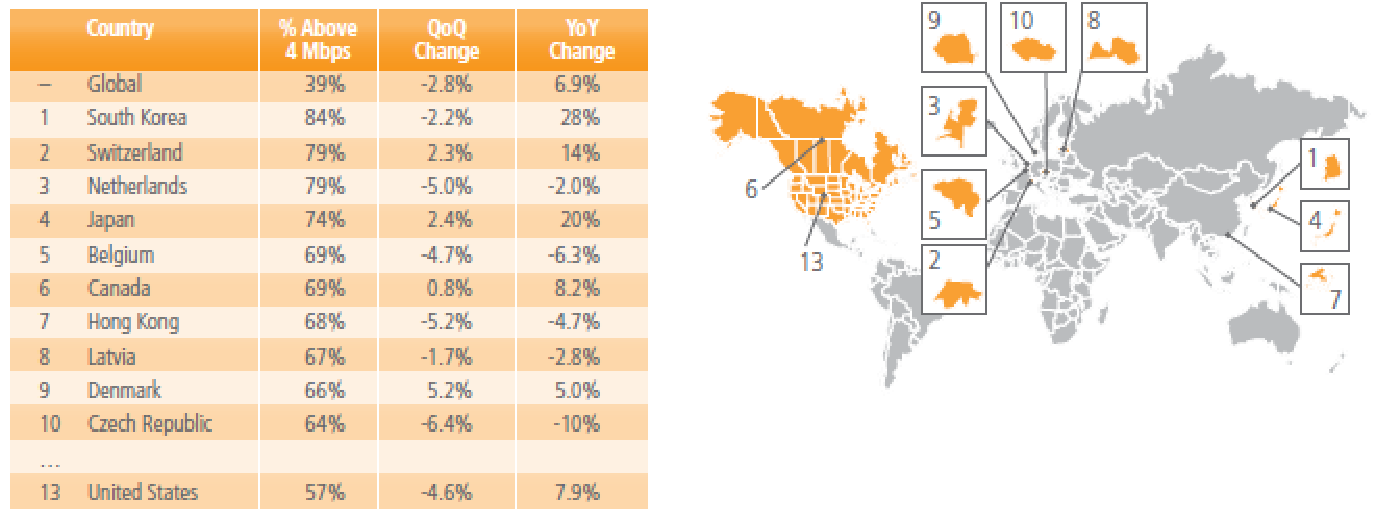
\includegraphics[width=1\textwidth]{./figures/internetstats.pdf}
      \caption[Broadband over 4Mbps connectivity statistics]{Broadband connectivity statistics about the speeds over 4Mbps around the globe.}
	\label{fig:bwWorldAvg}
\end{figure}

Regarding the specs on the client side, recent surveys and statistics taken by the game manufacturer Steam prove that more than  61\% of machines are carrying 1 to 4 gigabytes of RAM and nearly 90\% of computers handle 2 to 4 core CPU with a 64 bit OS~\cite{steamStats}, this environment can easily handle media enhanced applications that require high performance for media encoding. WebRTC concept rests over multiple layers having the browser as an underlying application, a traditional browser allocates a lot of resources for running being the performance of the machine a bottleneck in some cases.

Traditionally, WebRTC concept approaches rely on the usage of plug-ins or other separate software components that make the system run smoother by avoiding one layer of processing (browser) but being non-standard and not cross-compatible, one of the most import ant concepts when designing applications nowadays. This approach has a new alternative with the arrival of the new HTML5 where WebRTC is integrated as one of the new Application Programming Interfaces (APIs) available alongside other many different interesting capabilities.

\subsection{Background}

WebRTC API is included into the HTML5, this is the fifth version of the WWW language. This version includes different API's and JavaScript codes that help the developer to easily introduce new features into their already existing WWW applications. The initial HTML version (2.0) was published in November 1995 with the only goal of delivering static content from the server to client browser~\cite{html2IETF}. HTML became de de facto format for serving web information. 

HTML is written in tag formatting to identify different elements. Those tags are then interpreted by the browser to show the different data content served by the server. During the evolution of the WWW different new features have been added to the HTML standard and new versions where published, things like JavaScript and Style Sheets increase the flexibility and features of the WWW content enhancing the final user experience.

Due to the need to extend the features of the already existing HTML4 standard, a new version was proposed in 2004 by the Mozilla Foundation and Opera Software~\cite{initialHTML5proposition}. This new proposition focused in new developing technologies that could be backwards compatible with the already existing browsers, the idea didn't make a success and was tier apart until January 2008 when the first Public Working Draft was published by the Web HyperText Application Technology Working Group (WHATWG) in the W3C~\cite{firstHTML5draft}.

This proposal had a greater reliance in modularity in order to move forward faster, this meant that some specs that were included in the initial draft moved to different working groups in the W3C. Those technologies defined in HTML5 are now in separate specifications, one of them being WebRTC. WebRTC works as an integrated API within the browser that is accessible using JavaScript and is used in conjunction with the Document Object Model (DOM) interfaces. Some of the APIs that have been developed are not part of the HTML5 W3C specification but are included into the WHATWG HTML specification.

\subsection{Challenges}

WebRTC is a real time media protocol that will be obliged to share the available resources with many other applications. Due to the short experience in WebRTC congestion situations that share the available bandwidth with other existing solutions we will find some lack of documentation or previous literature regarding this topic. 

The aim to investigate and help to develop new protocols such as WebRTC is usually backed by a lack of information that may affect some of the statements made in this thesis. Hopefully, this won't affect the development of itself and the conclusions obtained at the moment of the development of the topic. 

Considering WebRTC is being developed at the moment of writing this thesis some of the statements made in here might be different in the following versions of WebRTC meaning that the problems analyzed have been solved.

\subsection{Contribution}

Investigate how WebRTC performs in a real environment trying to evaluate the best way to set multiple peer connections able to transfer media in different network topologies. Measure the performance of WebRTC in a real environment, identifying bottlenecks related to encoding/decoding, media establishment or connection maintenance. All this should be performed in real-time over a browser by using the already existing WebRTC API.

Using metrics related to RTT, latency, packet loss and bandwidth usage we expect to understand the way WebRTC performs when handling in different environments.

\subsection{Goals}

WebRTC uses and adapts some existing technologies for real-time communication. This thesis will focus in studying how:

\begin{itemize}
	\item WebRTC performs considering different topologies using video/audio acquired form the Webcam using the API and encoded using different codec types provided by the standard.

	\item Usage of WebRTC to build a real application that can be used by final users proving that the API is ready to be deployed and is a good approach for the developer needs when building real-time applications over the web. This will be done in conjunction with other new APIs and technologies introduced with HTML5.
	
	\item Testing of different WebRTC topologies with different network constraints to observe the response of the actual existing API.
\end{itemize}

The final conclusion will cover an overall opinion and usage experience of WebRTC, providing some valuable feedback for the needs and requirements for further modifications on the API.

\subsection{Structure}

Not sure about here

%documentation and drafts
%\section{Documentation and drafts}

%% 
%% Leave first page empty
\thispagestyle{empty}

Blah blah blah talk about the sdtrz process and APIs maybe? JSEP vs ROAP? CU-RTC-Web vs WebRTC? VP8 vs H.264 vs Optus? possible stuff to talk that might be interesting to introduce. Short and fast.

\subsection{CU-RTC-Web vs WebRTC}
In August 2012 Microsoft introduced his vision of a real-time communication between browser trying to cover all the WebRTC use cases with a different design \cite{curtcweb}, this draft collided directly with the ongoing WebRTC proposal done by the W3C working group \cite{webrtcW3cgroup}. W3C working group decided to attach to the already existing draft some aspects from the Microsoft proposal should be analyzed in comparison with WebRTC. Three main aspects differ from WebRTC:
\begin{itemize}
	\item No PeerConnection object
	\item No SDP description or JSEP
	\item No mantatory codec to be implemented
\end{itemize}
The ongoing WebRTC proposal identifies a Javascript object called RTCPeerConnection that handles and maintain all the peer connection data transfer, this object handles all the ICE, SDP creation, negotiation and transfer. In the CU-RTC-Web this concept is replaced with a proposal called RealtimeTransport interface that relies in a RemoteRealtimePort interface \cite{realtimemedia}. This design is a low-level API that forces web developers to build their own application-specific JavaScript code so it can be adapted to every different use case required. No API defined object like in WebRTC, more flexible but much more complicated to implement for application developers.

From the codec perspective CU-RTC-Web approach could be more sensitive to the codec war taking part on the workgroups, one of the key issues in the WebRTC standaritzation, not setting any codec to be mandatory makes sense considering that after long time there is no consensus about this position yet. On the other hand, it makes sense to set a mandatory codec for a media standard as it will force all the providers to set the same codec and avoid compatibility issues. Codecs being proposed are: VP8, H.264, Optus and G.711.

WebRTC draft RTCPeerConnection relies on a new Javascript spec called Javascript Session Establishment Protcol (JSEP) which help developers to handle the low-layer communication and negotiation tasks \cite{jsepIETF}. JSEP relies directly on the Session Description Protocol (SDP) \cite{sdpIETF}. CU-RTC-Web leaves freedom to developers to implement their own communication tasks for their specific application.

The conclusion shows that meanwhile WebRTC moves a lot of work to be done by the browser itself CU-RTC-Web leaves complete freedom to developers to adapt the use case to the proposal instead of adapting the application to the API such as in WebRTC. Both approaches can be valid, but WebRTC makes more sense form the developer point-of-view and it makes it easier to build applications on top of it.

%What is webRTC
\section{What is WebRTC?}

%% 
%% Leave first page empty
\thispagestyle{empty}

Web Real-Time Communication that builds P2P applications by using a defined API. The first announcement went public in a WG of the World Wide Web Consortium (W3C) in May 2011 \cite{webrtcW3cgroup} and started the official mailing list in April 2011 \cite{welcomeW3C}. During the first stage of discussion, the main goal was to define a public draft for the version 1 API implementation and a route timeline with the goal to publish the first version by March 2013. The first public draft of W3C came public the 27th of October 2011 \cite{originalW3Cdraft}. During this first W3C draft, only media (audio and video) could be sent over the network to other peers, it is focused in the way browsers are able to access the media devices without using any plugin or external software.

Alongside to the W3C working group, the WebRTC project also joined the IETF with a WG in May 2011 \cite{webrtcIETFgroup} with the first public announcement charter done the 3th of May 2011 \cite{webrtcIETFcharter}. Milestones of the WG initially marked December 2011 as deadline to provide the information and elements required to the W3C for the API design input. On the other side, the main goals of the WG covered the definition of the communication model, session management, security, NAT traversal solution, media formats, codec agreement and data transport \cite{webrtcIETFcharter}.

One  of the most important steps during the process of standardization came the 1st of June 2011 when Google publicly released the source code of their API implementation \cite{haraldpublicWebRTC}. 

During all this period both WGs have been working alongside to provide a reliable solution to enable cross-platform applications to perform media and data P2P transfer over the browser in a plugin-free environment. The first final version of the WebRTC API is to be published during March 2013.

\subsection{Support}

The following companies have supported and are actively working in the development of WebRTC standard in the W3C: Google, Mozilla and Opera \cite{googleAnnouncement}. Other companies such as Microsoft have supported browser-to-browser solution but have published their own proposal which differs with the one published in the WebRTC WG, called CU-RTC-Web \cite{curtcweb}, this proposal did not get much traction by the workgroup being declined to unify with the current specs, during an W3C workgroup poll in September 2012 the chairs of the group decided to attach to the already existing WebRTC API instead of moving it to the CU-RTC-Web \cite{curtcpoll}.

During the firsts attempts to build a reliable solution for WebRTC Ericsson Labs presented an initial API based on the preliminary work done in the WHATWG, this API was called ConnectionPeer API and required an special module to be installed in your browser \cite{ericssonwebrtc}. Ericsson lately dropped from the effort to build it's own browser to focus in the standardization and codec discussion, leaving the API implementation to the Mozilla and Chrome teams. The original API evolved rapidly during the next months thanks to the WGs and the developer community feedback that is experimenting with the unstable API.

\subsection{Milestones}

During the process of standardization some important moments should be remarked. In January 2012 Opera implemented the first version of WebRTC getUserMedia for accessing the camera and audio \cite{operaannouncement}, during this year getUserMedia is available in the stable version of Opera. 

Google Chrome integrated the first version of WebRTC in its DEV and Canary channels of the browser during January 2012 \cite{chromeannouncement}, in June 2012 it started moving its API to the stable channel hidden behind a flag, in November 2012 WebRTC becomes fully available in Google Chrome stable channel and is open for public usage \cite{chromestable}. 

Mozilla Firefox started working on the getUserMedia implementation early 2012 delivering the first version of media access trough API at the beginning of 2012 in the alpha version \cite{mozillablog}, in April 2012 Mozilla published a WebRTC video demo running on Firefox in the "adler" channel \cite{mozillawebrtc}, also supporting some primitive DataChannel API. Later in October Firefox Nightly was carrying the first unstable version of the WebRTC API including DataChannel \cite{mozillafinal}, Mozilla announced in September 2012 that the stable version of WebRTC will be shipped along with Firefox 18 in January 2013 \cite{mozillacomming}. 

Some announcements done from Microsoft point out that they are also working in some implementation into Internet Explorer by using CU-RTC-Web as the default standard, at the moment only the Media API information is publicly available \cite{microsoftcapture}.

In October 2012 Ericsson announced the world's first WebRTC-enabled browser for mobile devices called "Bowser" with support for iOS and Android, this browser is able to handle WebRTC calls using RTCWeb Offer/Answer Protocol (ROAP) which is an old discontinued version of the WebRTC API that has moved to Javascript Session Establishment Protocol (JSEP). This browser also differs from the previous desktop alternatives on the codec side, it is carrying H.264 for video and G.711 for audio \cite{ericssonbowser}. The API provided by Bowser is not fully W3C compliant.

\subsection{Alternatives}

Some alternatives are available to the WebRTC concept, considering the global architecture of WebRTC, Session Initiation Protocol (SIP) and Secure Real-Time Media Flow Protocol (RTMFP) are similar approaches to the same solution.

\subsubsection{SIP}

Both SIP and RTMFP are protocols to allow communication between two different users with audio/video support. SIP is an open standard and RTMFP is a proprietary protocol by Adobe, both systems are widely used for real-time communication. SIP final Request for Comments (RFC) was published in June 2004 \cite{sipRFC}, this chapter describes the methods and behaviors of SIP. From an overview perspective, SIP is an application-layer control protocol for multimedia sessions, can establish, maintain and terminate them, during the development of the standard different new functionalities were added to the drafts such as conferencing and the possibility of adding/removing media from existing sessions. SIP differentiates from RTMFP/WebRTC by locating the end user to be used for communication, this feature allows SIP to be closely related to traditional PSTN networks as it allow cross-domain communication which is not possible when using RTMFP/WebRTC. SIP is not a complete toolkit for communications, it works alongside with other existing protocols such as Real-time Transport Protocol (RTP), Real-Time Streaming Protocol (RSTP), Session Description Protocol (SDP) and Media Gateway Control Protocol (MEGACO). Using SDP for the session negotiation between the end-points and RTP/RSTP for the media transport, all those protocols usage is widely extended in the network and provides legacy for older technologies. Meanwhile SIP can locate and deliver a message to a user, SDP can provide the required information for the session establishment and RTP can transport the type of media specified in the SDP body.

\begin{figure}[h]
  \centering
    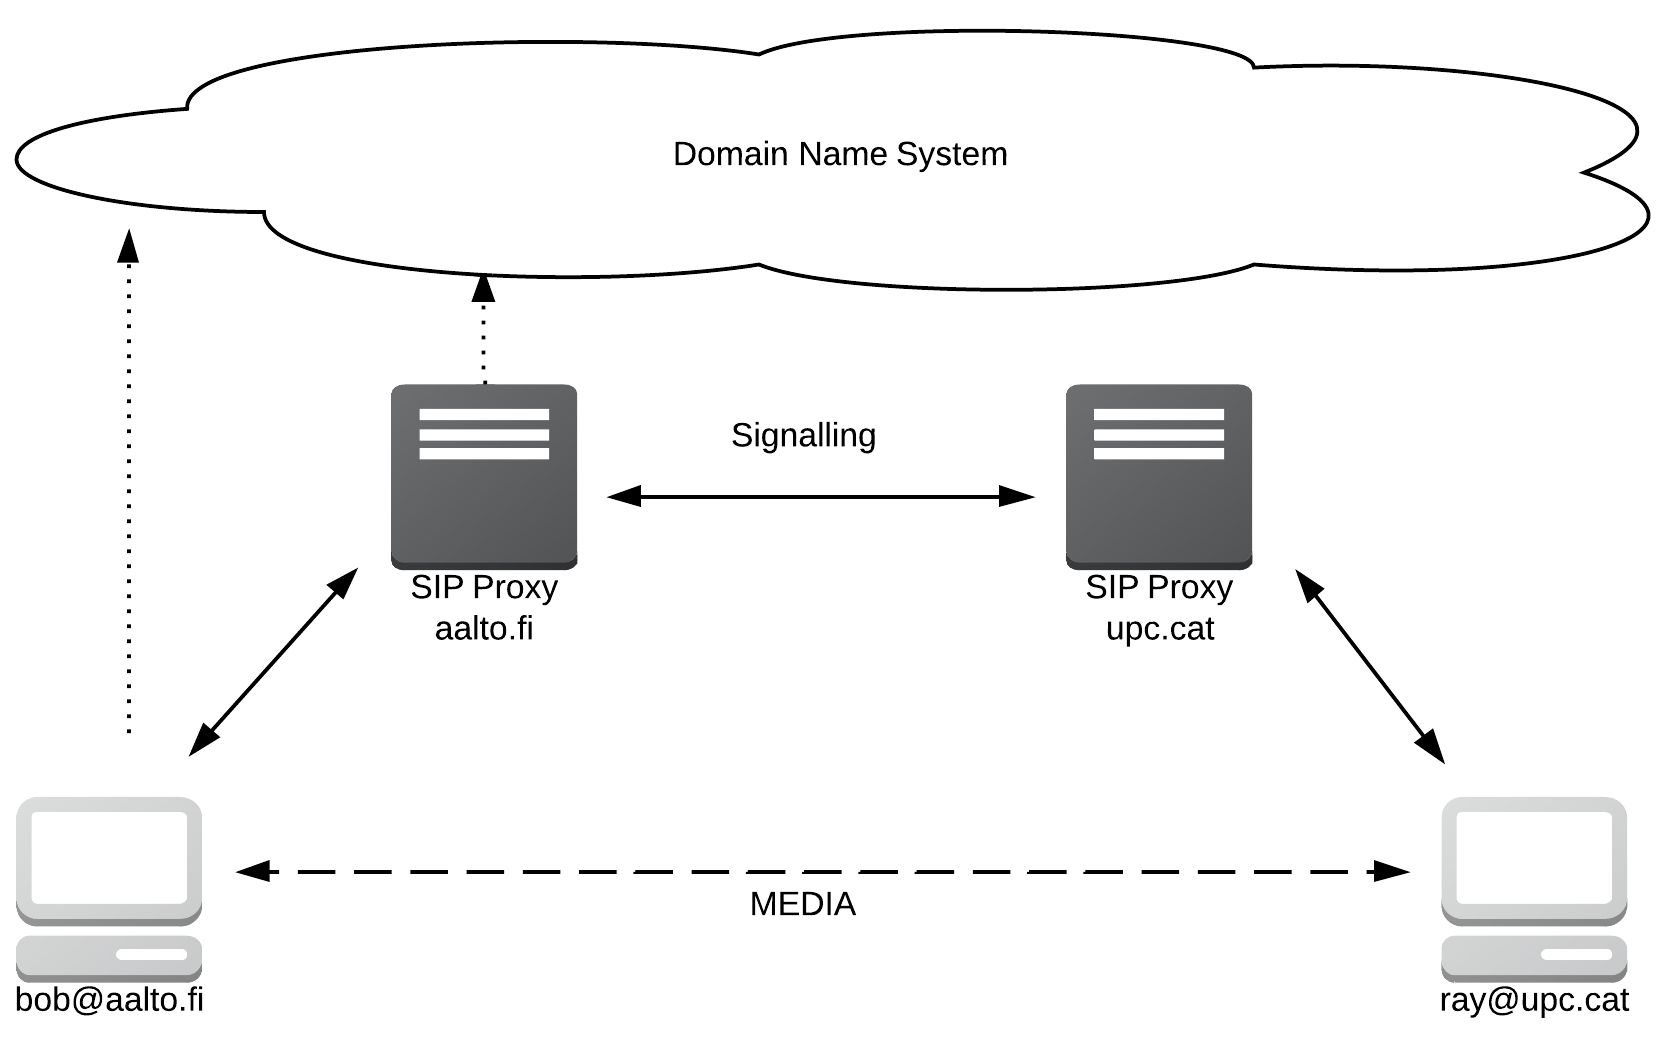
\includegraphics[width=1\textwidth]{./figures/SIParchitecture.png}
      \caption[SIP architecture for end-to-end signaling]{SIP architecture for end-to-end signaling.}
	\label{fig:SIParchitecture}
\end{figure}

SIP architecture relies in a trapezoid form where the Domain Name System (DNS) is used to locate the other peers of the system, once that peer is located and session is negotiated, media flows peer-to-peer directly to the endpoint. In order to build this system different agents are needed, SIP Proxies, SIP Redirect and SIP Registrar. SIP Proxies transmit the SDP and SIP messages from one peer to the other to establish communication (Figure ~\ref{fig:SIParchitecture}). SIP Registrar are the machines that collect and save all the user information from the end points.

DNS provides the IP address for both proxy servers and allow the messages to be exchanged between both peers, when SIP is used the following messages are exchanged: INVITE, RINGING and 200OK. Those messages carry the SDP data inside in an object format, when ray@upc.cat receives the INVITE message from bob@aalto.fi builds the 200OK response carrying the SDP object that providing compatibility check between both peers and which options and codecs to use. SIP provides some more messages to update the already existing session or to close them. The media transport is done using RTP and RTCP that rely over User Datagram Protocol (UDP) \cite{sipRFC}.

SIP is a pure Voice Over IP (VoIP) confederated technology that helped the community to learn about real-time P2P communication,we have used all the concepts and technologies embedded in SIP to build WebRTC.

\subsubsection{RTMFP and Adobe Flash}

RTMFP and Adobe Flash are proprietary technologies provided by Adobe, both services work together to provide multimedia and real-time communication between users.

Adobe Flash is a multimedia software that uses a plugin to work over the browser, it is used to build multimedia experiences for end users such as graphics, animation, games and Rich Internet Applications (RIAs). It is widely used to stream video or audio over webpages, in order to reproduce this content we need to install Adobe Flash plugin in our computer. It also carries different programming languages that drops from the standards called JavaScript Flash Language (JSFL) and ActionStript. Due to the need of using a plugin his extension to tablets and mobile devices is more complicated than using standards. Adobe Flash Player is available in most platforms except iOS devices and reaches about 98 of all internet-enabled desktop devices. This plugin allows developers to access media streams from external devices such as cameras and microphones to be used along with RTMFP.

RTMFP uses Adobe Flash to provide media and data transfer between two end points. This system usually works over UDP \cite{rtmfpDraft}. Differing from SIP, this protocol is a full suite for media/data transfer in a P2P constraint environment and carries its own signaling methods and codecs. It also handles congestion control on the packets and NAT transversal issues. One of the biggest differences is that, similar to WebRTC, is not a full communication infrastructure and both peers must be in the same working domain to be able to communicate, is not a PSTN style of communication but a point to point messaging system. This protocol is implemented in Flash Player, Adobe Integrated Runtime (AIR) and Adobe Media Server (AMS)  \cite{rtmfpDraft}, it is used for P2P communication between all those services. 

This protocol is secured and encrypted, comparing with WebRTC, this issue has been addresses clearly in RTMFP by using proprietary algorithm and different methods. The RTMFP architecture is similar to WebRTC concept, it also allows reconnection in case of connectivity issues and works by multiplexing different media streams over the same media channel when handling conferences or multiple streams. For the signaling part Adobe uses a service called Cirrus (Figure ~\ref{fig:RTMFParchitecture}), this service allows architectures such as: end-to-end, many-to-many and multicast \cite{cirrusFAQ}.
 
 \begin{figure}[h]
  \centering
    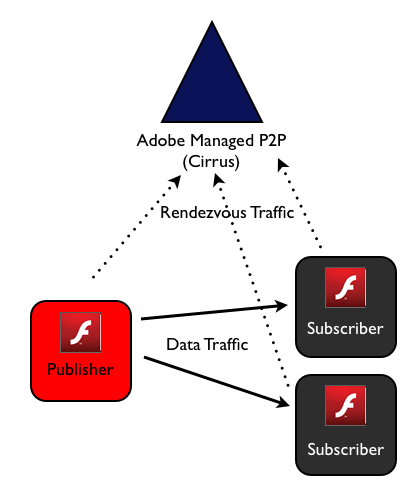
\includegraphics[scale=0.6]{./figures/cirrusAdobe.jpg}
      \caption[RTMFP architecture using Cirrus (source: Adobe)]{RTMFP architecture using Cirrus (source: Adobe).}
	\label{fig:RTMFParchitecture}
\end{figure}
 
Some of the most valuable features is the possibility to easy integrate P2P multicast topologies where one source sends a video to a group of receivers. This is something that none of the other protocols has implemented yet.

\subsection{HTML5}

WebRTC is part of the HTML5 package, both combined are an open cross-platform standard that aims to replace the Adobe proprietary proposal for P2P Real-Time Communication (RTC).

By using HTML5 features we avoid the need of installing any extra software to be able to use real-time multimedia applications on the browser.

\subsubsection{Media Capture and Streams}

HTML5 proposal will replace the existing need to use plugins when having multimedia features in web browsers. This new version carries different API that will be built into the browser and avoid the usage of external software to execute them, this scenario helps to build cross-platform standard applications in JavaScript instead of using plugins. 

Compared with the existing Adobe Flash, APIs such as Web Graphics Library (WebGL) enables developer to build HTML5 3D and 2D games that will work in any browser natively without needing any especial software but with the rendering capabilities of Flash. Mobile browsers have been more likely to adopt this new technology for rendering \cite{webglDraft}. The first final version of the API has been already published and browsers like Chrome and Firefox carry it.

Alongside with WebGL and many other APIs, this new HTML5 also carries the new Media Capture and Streams, also known as GetUserMedia API. This JavaScript API allows developers to access local media such as video/audio from webcams and insert them in a web application by using the new video DOM element \cite{getusermediaDraft}.

This proposal was first attached directly to the WebRTC group but has been published in a different draft, the usage of this API removes the need of using Adobe Flash to access the media device and also the plugin requirement. Developers can capture media streams from cameras and build them into Blob objects to be transmitted to other peers or reproduced locally.

 \begin{figure}[h]
  \centering
    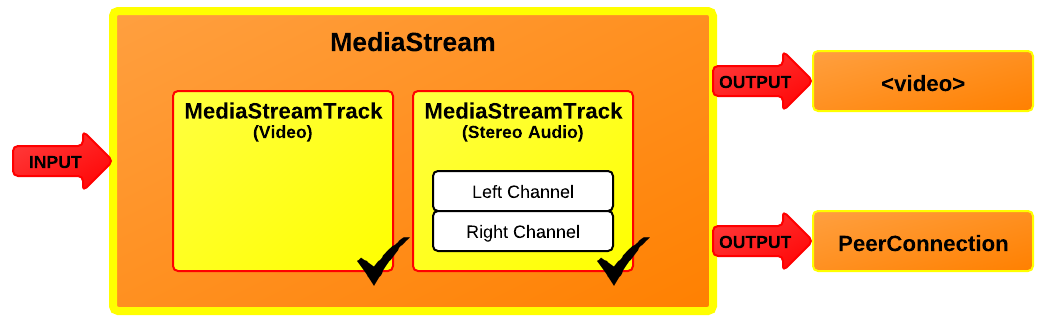
\includegraphics[scale=1]{./figures/mediastreamAPI.png}
      \caption[Media Stream API (source: W3C)]{Media Stream API (source: W3C).}
	\label{fig:mediastreamAPI}
\end{figure}

Figure ~\ref{fig:mediastreamAPI} illustrates how the browser access that media and the outputs delivered to the developer. We will use this function to build WebRTC enabled applications for RTC video conferencing. The video tag is an HTML5 DOM element that reproduces local and remote streams.

\subsubsection{WebRTC}

WebRTC is a working API part of the HTML5 proposal, it is defined in a W3C draft \cite{webrtcW3cgroup}. This API replaces the need of a RTMFP plugin for P2P communications for browsers, WebRTC uses already existing technologies, learned from SIP, bundled into an API. It is able to solve NAT transversal environments by using a mixtures of ICE, TURN and STUN technologies. For the session description it uses a modified bundled version of SDP. The format used for packet transport is RTP and SRTP, modified WebSockets are in use for P2P DataChannel implementation to provide data transport multiplexed over the same stream. All the traffic is sent over UDP or TCP \cite{alvestrandOverview2012}.

This P2P session establishment system works in a constrained environment similar to RTMFP but it has been designed to provide legacy for other SDP based protocols such as SIP. It is a browser side API and does not provide any centralized service for signaling. Figure ~\ref{fig:webrtcExample} shows how a WebRTC simple P2P scenario works, the server used for signaling is based in node.js.

 \begin{figure}[h]
  \centering
    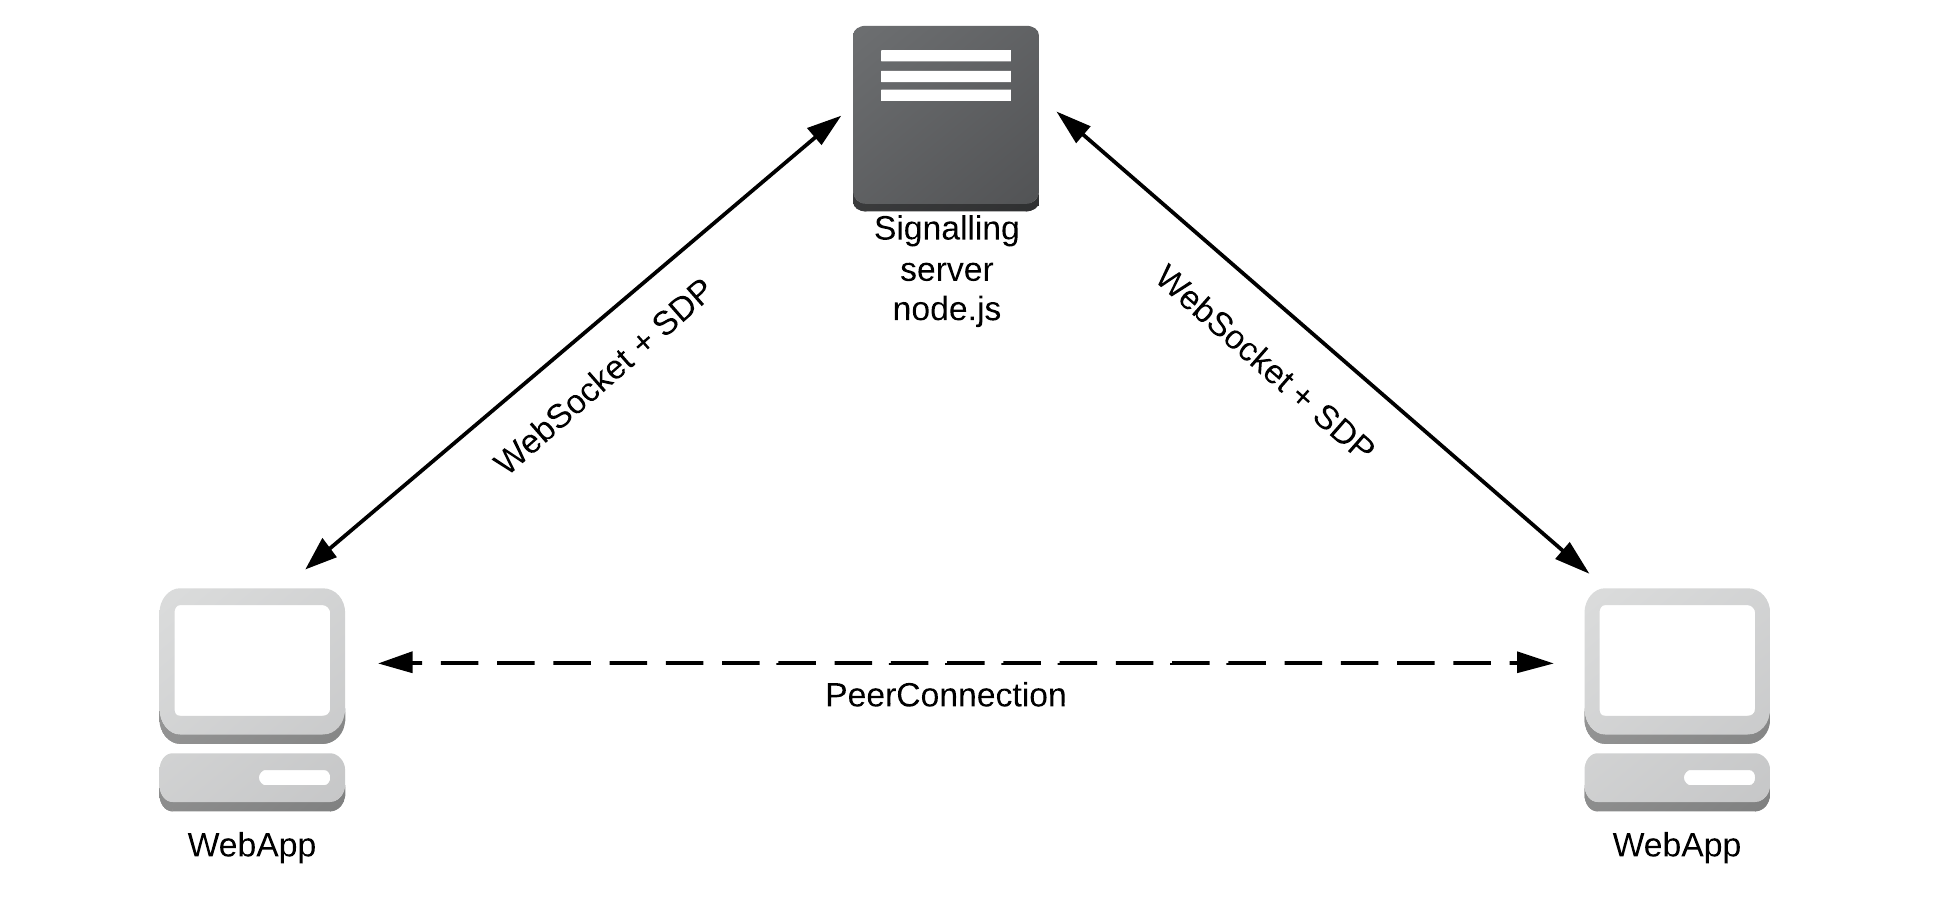
\includegraphics[width=1\textwidth]{./figures/webrtcExample.png}
      \caption[WebRTC simple topology for P2P communication]{WebRTC simple topology for P2P communication.}
	\label{fig:webrtcExample}
\end{figure}

Figure ~\ref{fig:webrtcExample} does not show relay machines that provide NAT transversal solutions, those rely in other technologies that are applied to the API. In this simple example we consider both peers are in the same network without any Firewall or NAT restriction.

\subsection{Issues in WebRTC}

WebRTC uses a mixture of different technologies to perform peer-to-peer communication between clients, those technologies range from SRTP, RTP, RTCP and multiple codecs that are being discussed. This scenario makes performance the key point for success in developing stable WebRTC applications. 

Performance is manly related to computer capabilities and the ability to encode/decode at the same time as transferring and monitoring multiple peer connections. All those tasks are run over the browser and not directly on the OS, this is good for interoperability between platforms but bad in the performance aspect. Compared to Adobe technologies which uses a plugin, the performance they can deliver should be higher as they do not use as many application layers.

Media applications are delay sensitive and require a low packet loss for its proper function, WebRTC is working on this aspect by trying to implement congestion control over the connection stablished between peers, this work is not completed yet and will arise as a problem in the near future. Packet loss due to system capacity and bandwidth are measurable in WebRTC using the Stats API, this API provides information about the PeerConnection performance and is accessible by JavaScript.

Media constraints and bandwidth statistics will make a big difference in how media is acquired in WebRTC. Browsers and web applications have always tolerate some amount of delay and packet losses but this is not possible in media infrastructures for real time applications, an effort is needed to handle Quality of Service (QoS) in WebRTC to compete with RTMFP.

\subsubsection{Quality of Service}

Quality of Service (QoS) for WebRTC is being discussed and an internet draft is available with some proposals \cite{qosWebRTCIETF}. WebRTC uses DiffServ packet marking for QoS but this is not sufficient to help prevent congestion in some environments. Packet marking will help in Wifi and broadband connections but will not be very useful in mobile networks as marking could be removed by the provider. Audio/video packets will be marked as priority using DSCP mappings with audio being more important than video or data \cite{qosWebRTCIETF}. 

The possibility to combine QoS in the transport layer with the constraints and stats of the WebRTC API will help developers to build more adaptive applications, for example, lowing the Frames per Second (FPS) in the case of high packet losses will reduce the bandwidth usage in the case of congestion of the link. This is possible thanks to the Stats API that provide the data statistics for the peer connection.

Some environments will also require better QoS as their bandwidth will be lower, examples in the use case draft relate this to surveillance cameras or similar approaches \cite{WebRTCcasesIETF}. In these cases QoS should be modified by using the API, this situation can lead also to malicious JavaScript injection that could flood the path with packets. 

\subsection{Security concerns}

In order to establish a call in WebRTC we use a web server for the signaling part, on the browser side we rely on built-in standardized JavaScript calling APIs which are used by the web server to establish the call between two peers \cite{WebRTCcasesIETF}. Figure ~\ref{fig:webrtcExample} represents the simple topology for a WebRTC call, even this system is similar to other provided VoIP services, the web server is able to move logic from the JavaScript in the browser giving total control to the server.

Obviously, this system poses a range of new security and privacy challenges different from traditional VoIP systems. It has to avoid malicious calling or having a call established without user knowledge, considering that those APIs are able to bypass Firewalls and NAT, Denial of Services (DoS) attacks are a threat.

Nowadays browsers continuously execute JavaScript codes from accessed web sites, this also includes malicious scripts, but in the case of WebRTC this could lead to a big privacy threat. In a WebRTC environment we consider the browser to be a trusted unit and the JavaScript provided by the server to be unknown as it can execute a variety of actions in the browser. At minimum, it must not be possible for arbitrary sites to initiate calls to arbitrary locations without user consent \cite{rtcwebSecurityIETF}. To approach this, the user must make the decision to allow a call (and the access to its webcam media) with previous knowledge of who is requesting the access, where the media is going or both.

The previous procedure is run by the JavaScript provided by the server, this is a security issue as the user must trust an unknown authority server. Calling services commonly use HTTPS for authentication whose origin can be verified and users should be verified cryptographically (DTLS-SRTP). Browser peers should be authorized before starting the media flow, even this can be done by the PeerConnection itself by using some Identity Provider (IdP) that supports OpenID or BrowserID to demonstrate their identity \cite{rtcwebSecurityArchIETF}. Usually this problem is not particularly important in a closed domain, cases where both peers are in the same social network and provide their profiles to the system and those are exchanged previous to the call, but it arises as a big issue when having federated calls from different domains.

If the web service is running over a trusted HTTPS certificate and has been authenticated it will be possible for the user to set the allow always access to the media, otherwise the user will have to allow this access. Once the media is acquired the actual API builds the ICE candidates for media verification. Authentication and verification in WebRTC is an ongoing discussion in the WG.



%Use cases and topologies
\section{Topologies}
\label{sec:topologies}


%% 
%% Leave first page empty
\thispagestyle{empty}

We will talk about the different topologies that will be studied in this document that use WebRTC.

\subsection{Point-to-Point}

Point-to-point environments are widely used as a private calling system between two individuals, when related to WebRTC those use cases can be extended to people in the same domain so it is not required to be as private as other technologies. 

Support systems are being considered as a valuable scenario for WebRTC point-to-point calls, this method will be useful as WebRTC does not need any plugin or account setup if we want an easy way to provide support to our customers in an HTML5 enabled site.

Other similar uses could be communication between doctor and patient in a medical application that intends to be cross-platform compatible in an ongoing standard. Communication in other scenarios such as citizens and authorities could also rely in a WebRTC application.
 
\subsubsection{Challenges}

In this scenario most challenges will come from the networking aspect. We could consider the enterprise use case, we will have ongoing calls between workers in the same enterprise network, this network could be restrictive to the use of non-trusted STUN servers or it might drop the UDP packets. Having restrictive NATs or Firewalls will directly affect the possibilities of having the WebRTC call correctly established, in this situation the possibilities of success highly rely on the network used.

When having point-to-point calls the problem that could arise from the local performance on the machine is not that critical considering that only one peer connection will be handled carrying two to three streams. We will focus on the user experience when having high restrictions in the NAT/FW.

\subsection{One-to-Many}

One-to-many scenarios are widely known as a type of multicast, one source sends the media to the different clients that connect to the origin. When having this topology the common uses rely on video and audio streaming to multiple clients, TV channels and streaming conferences are popular.

For example, we could have a major sport even being retransmitted to the viewers by using one-to-many. Other solutions could cover the use of WebRTC to have a CEO talking to the employees by using an HMTL5 web application. Music bands also could take advantage of this scenario by being able to transmit his show to the audience.

\subsubsection{Challenges}

In this scenario we will have a video, audio and data streaming connection from one source to multiple devices. This will cause a huge load on the source when having multiple PeerConnections running, local performance will be a constraint. Considering other scenarios, in this case, latency on the network is not as important as the rest due to the one-way communication only, no video and audio is needed to be received on the source.

We will need to study ICE and STUN mechanisms and how they perform in this scenario but the problems will arise from the source capacity on the hardware and link. Bandwidth demand on the source will be high and may affect the communication. On the other hand, having the audio delayed a couple of seconds is not going to affect the user experience in the call.

From the client perspective, the PeerConnection stablished will be easy to handle as no RTP streams will be sent back to the source, except the RTCP messages.

\subsection{Many-to-Many}

Many-to-many topologies are used for conferencing environment, this topology is used in systems such as Skype or VoIP. Conferences are used in enterprises for long-distance communication between employees and working groups, by this, the need of having those calls working smoothly for all participants is very important.

Due to the compatibility with HTML5 and the DataChannel spec that is shipped with WebRTC many-to-many environment could be also used for data transmission between different peers in a torrent scenario. Combining it with WebGL it could even be used for gaming experiences or file sharing.

\subsubsection{MCU}

MCU usage will surely be an option when designing WebRTC infrastructures, the ability to multiplex different streams into the same channel will directly affect on how the client performs when reproducing the video reducing the amount of used resources. 

\subsubsection{Challenges}

When running multiple peer connections browsers on the client side will be obliged to handle multiple incoming streams and keep up all the connections stablished, this will be a problem regarding to the resources on the client side. 

So, alongside with other problems mentioned in previous topologies, resources will directly affect on how this scenario performs in different users. 

On the other side, even considering that NAT and Firewall connectivity issues are solved, we should be careful when guaranteeing all peer connections to be correctly stablished. TURN/STUN failures might directly affect to the success ratio in this topology.



%Congestion environments
\section{Key Performance Indicators in Real-Time Environment}


%% 
%% Leave first page empty
\thispagestyle{empty}

This section will define the way we measure the performance in WebRTC environments, this real-time media environment will require an specific approach and some metrics to define how the protocol behaves in different topologies and scenarios. 

Different issues might affect directly how the WebRTC media performs, these range from the hardware of the clients to the state of the link. In the following chapters we will describe some of them that will be used in our study cases.

\subsection{Losses}

Loss rate indicates packet losses during the transmission or processing. Usually packet losses affect directly the performance of a call and can indicate how the link is behaving between the different peers, in our case, packet loss will be a direct indicator of the quality of the ongoing WebRTC transmission. However, the packet loss indicate that some packets are not arriving, another strong indicator that goes attached is delay as packets will arrive later prior to getting lost in the link. This indicator will show up when the link is carrying big congestion of failures. 

Some delayed packets should also be considered as losses as they won't be useful anymore for the ongoing connection, those packets won't show up in the stats as losses. In WebRTC loss rate will affect directly to the ongoing transmission as the delay range that we can tolerate is very low before the quality of the call deteriorates, some data-driven WebRTC connections will tolerate some more delay. In general case Loss Rate will be considered as a main point for recalculating the path by using faster routes. This indicator is manly attached to link quality.

Losses will be calculated in a certain period of time so we will be able to see how much loss rate we have in a certain range of time.

\begin{equation}
	\frac{PKT_{loss}(T) - PKT_{loss}(T-1)}{PKT_{received}(T) - PKT_{received}(T-1) + PKT_{loss}(T) - PKT_{loss}(T-1)}
	\label{eq:PKTloss}
\end{equation}

Equation~\ref{eq:PKTloss} calculates the estimated packet loss we might have on the link. This operation will be done every period, we will determine this period when building the testing environment.

\subsection{Round-Trip Time (RTT)}

The delay in a link can be measured form different perspectives, one-way delay indicates the time it takes for a packet to move from one peer to the other peer, this time includes different delays that are given in the link. This one-way delay is calculated form the time taken to process it in both sides (building and decoding), the lower layer delay in the client (interface and intra-layering delay), queuing delay (from the multiple buffers in the path) and propagation delay (speed of light). The sum of all those delays compose the total one-way delay.

Considering the structure of WebRTC, one of the most important delays that we will have to consider and study is the processing delay as our applications will rely in a multiple layer structure, running over the browser will affect the performance compared to other technologies that run directly over the OS. Delays in our case will be symmetric as we will be sending and receiving media, the delay will be important in order to reproduce the streams in the best quality possible and avoid decoding artifacts in the media. 

RTT will be an early indicator of congestion in a WebRTC connection, this RTT must be monitored and most important, the adequate RTT have to be defined for every connection as the clients won't be aware of the appropriate amount for good performance.

\subsection{Throughput}

Throughput will be a key metric for testing the performance of WebRTC environments, this value will show how much capacity of the link is taking each PC and stream. It is complex though as there is still no QoS implemented in WebRTC. The throughput metric is going to provide bandwidth for video/audio in each direction, we can then use this value to provide some quality metric averaging all the previous mentioned measures in order to monitor the overall quality of the call. A sudden drop of the throughput will mean that the bandwidth available for that PC has been drastically reduced, this will lead to artifacts, or in the word case, loose of communication between peers. In this specific situation ICE candidates will try to be renegotiated in order to obtain a different solution for the connection and reestablish the media with the best throughput possible.

\subsubsection{Audio streams}

When using real time media environments for bidirectional communication the user experience is a key indicator of success. One of the factors that have to be considered is the Noise Reduction (NR) and Acoustic Echo Canceler (AEC). Those mechanisms allow the call to be smooth and avoid extra noises and echoes from the speaker voice to be transmitted, in WebRTC will provide a strange behavior when measuring the throughput, when the is no speech the bytes transferred will be approximately zero, being the throughput negligible. This helps to reduce the bandwidth usage and provides a more comfortable conversation when having a call.



%Simulation environment
\section{Testing Environment}
\label{sec:testingEnv}

%% 
%% Leave first page empty
\thispagestyle{empty}

This chapter will describe which tools will be used to run the performance tests in WebRTC, different tools will be used.

\subsection{Stats API}

WebRTC carries a subsection of methods to help developers to access the lower layer network information, this methods return all different types of statistics and performance indicators that we will be using to build our own JavaScript Stats API. When using those statistics we will measure all the congestion KPIs to analyze them.

The method used is the RTCStatsCallback returns a dictionary object (JSON) that has be parsed and manipulated to get the correct indicators, this object returns as many streams as available in a PeerConnection, usually audio and video. This data is provided by the lower layers of the network channel using the RTCP packets that come multiplexed in the RTP stream~\cite{rtpusageIETF}.

The Stats API is the way that WebRTC allows the developer to access different metrics, as this is still in an ongoing discussion the stats report object has not been totally defined and can slightly change, the methods used by the Stats API are available on the W3C editors draft ~\cite{editorWebRTCdraft}. 

We have built a JavaScript tool that uses those stats from the browser to calculate the RTT, throughput and loss rate for the different streams that are being received. Those stats can later be saved into a file or sent as a JSON object to a centralized monitoring system. Our JavaScript grabs any PeerConnection passed through the variable and starts looping an iteration to collect those stats and either plot them or save them into an array for post-processing. 

Figure~\ref{fig:onetooneWifiRTC} shows an example capture of a call between two browsers in two different machines, Mac and Ubuntu, the call was made over Wifi open network with no firewall in the middle but with real traffic. The measures are directly obtained from the Stats API JS file we have built and post-processed using {\it gnuplot}.

 \begin{figure}[h]
  \centering
    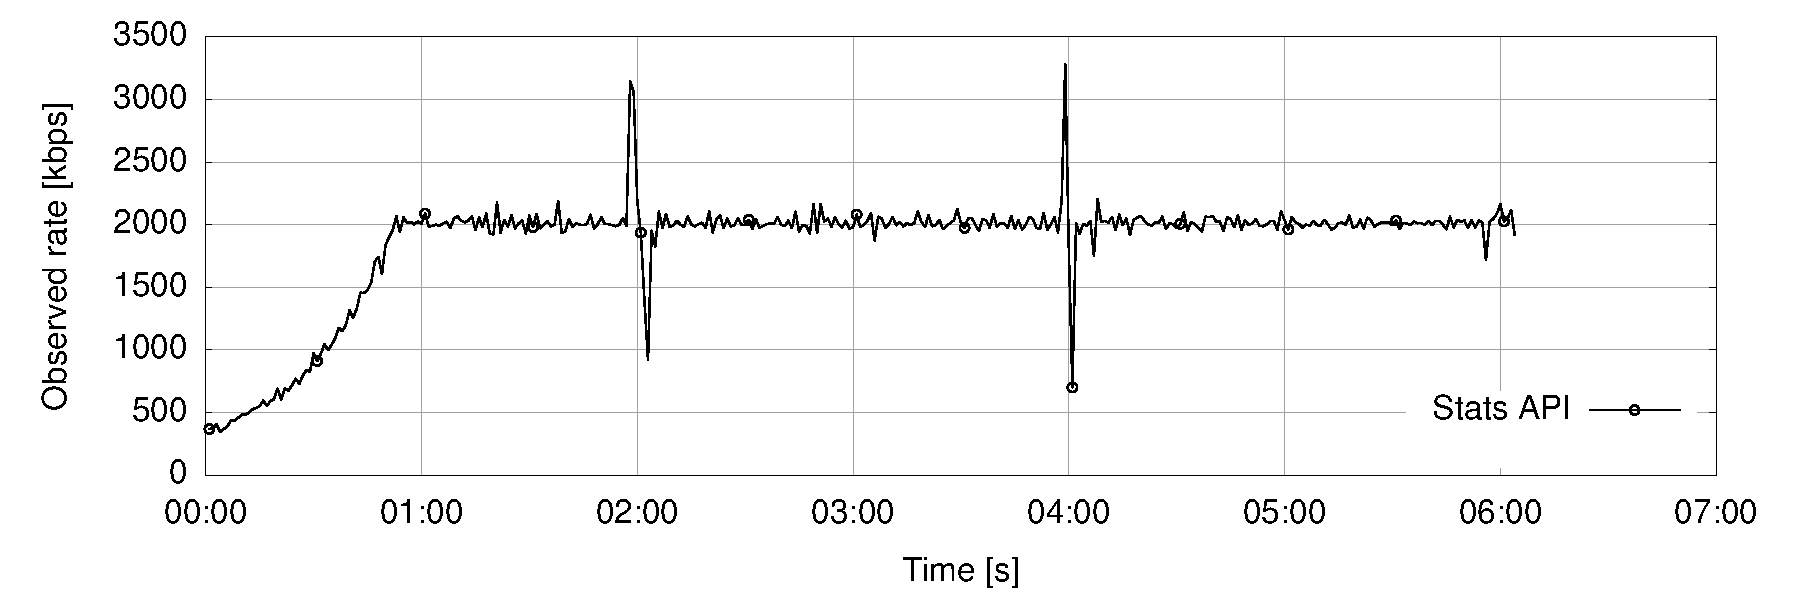
\includegraphics[width=1\textwidth]{./figures/onetooneWifiStatsRTC.pdf}
      \caption[Point-to-point WebRTC video call total throughput graph using Stats API over public WiFi]{Point-to-point WebRTC video call total throughput graph using Stats API over public WiFi.}
	\label{fig:onetooneWifiRTC}
\end{figure}

The previous Figure~\ref{fig:onetooneWifiRTC} considers the global bandwidth of the call, this means that the input/output video and audio are measured together to check how much bandwidth is being consumed over the duration of the call, as it is using RTCP packets for the metrics it takes a while to reach the average rate value. We can then plot all the different streams together to get an idea of how much bandwidth is consuming every stream.

 \begin{figure}[h]
  \centering
    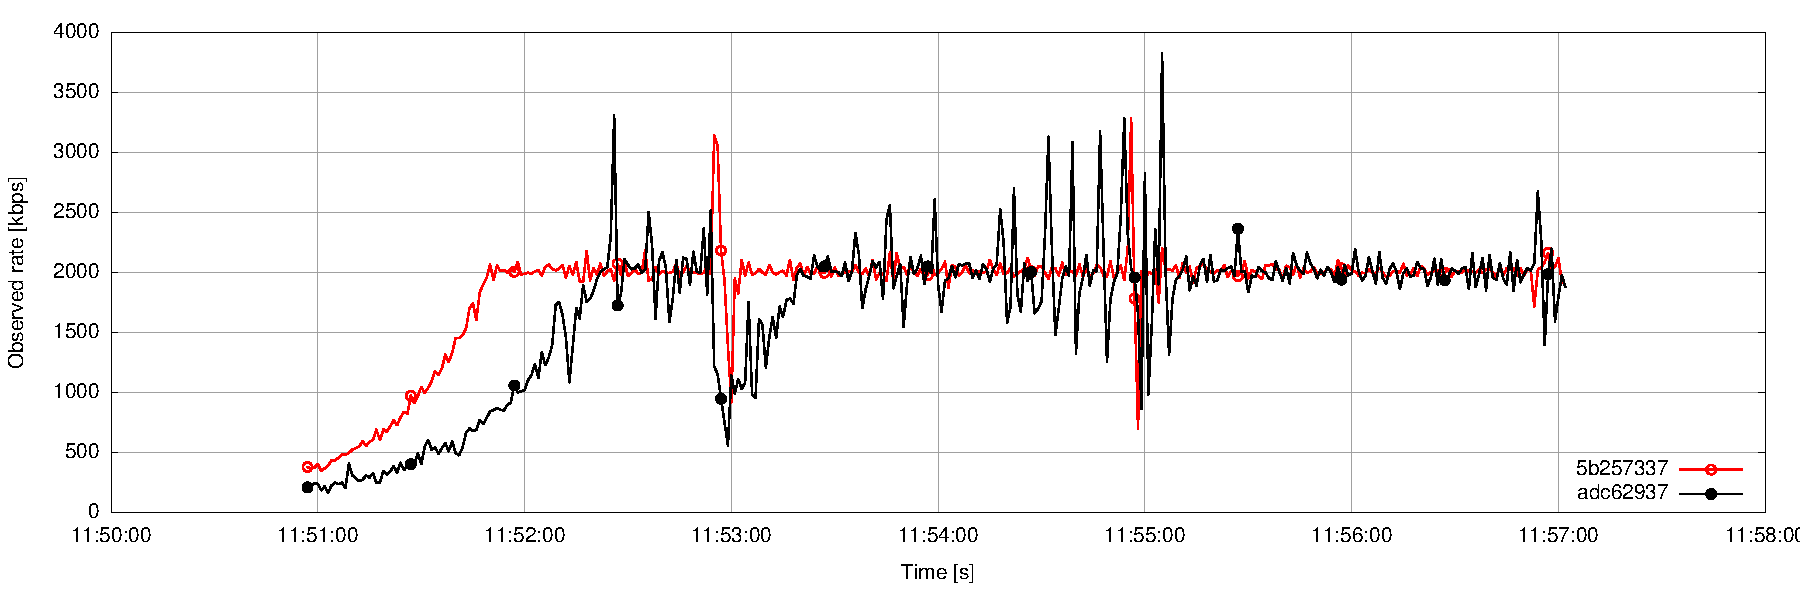
\includegraphics[width=1\textwidth]{./figures/onetooneWiFIStatsVideoStreams.pdf}
      \caption[Point-to-point WebRTC input/output video throughput graph using Stats API over public WiFi]{Point-to-point WebRTC input/output video throughput graph using Stats API over public WiFi.}
	\label{fig:onetooneWifiRTCVideoStreams}
\end{figure}

Figure~\ref{fig:onetooneWifiRTCVideoStreams} shows the two video streams captured from the same machine, one is outgoing the local video stream meanwhile the second stream is the incoming video stream from the other peer. We have built a flexible processing system that allows us to capture and analyze all the possible combinations of streams and metrics. The timing used for the capture is provided by the TimeStamp available on the RTCP. The average bandwidth used in this scenario of point-to-point call in a standard wireless network is around 2000 Kbps per video stream. Both figures are plotted from the same original call.

 \begin{figure}[h]
  \centering
    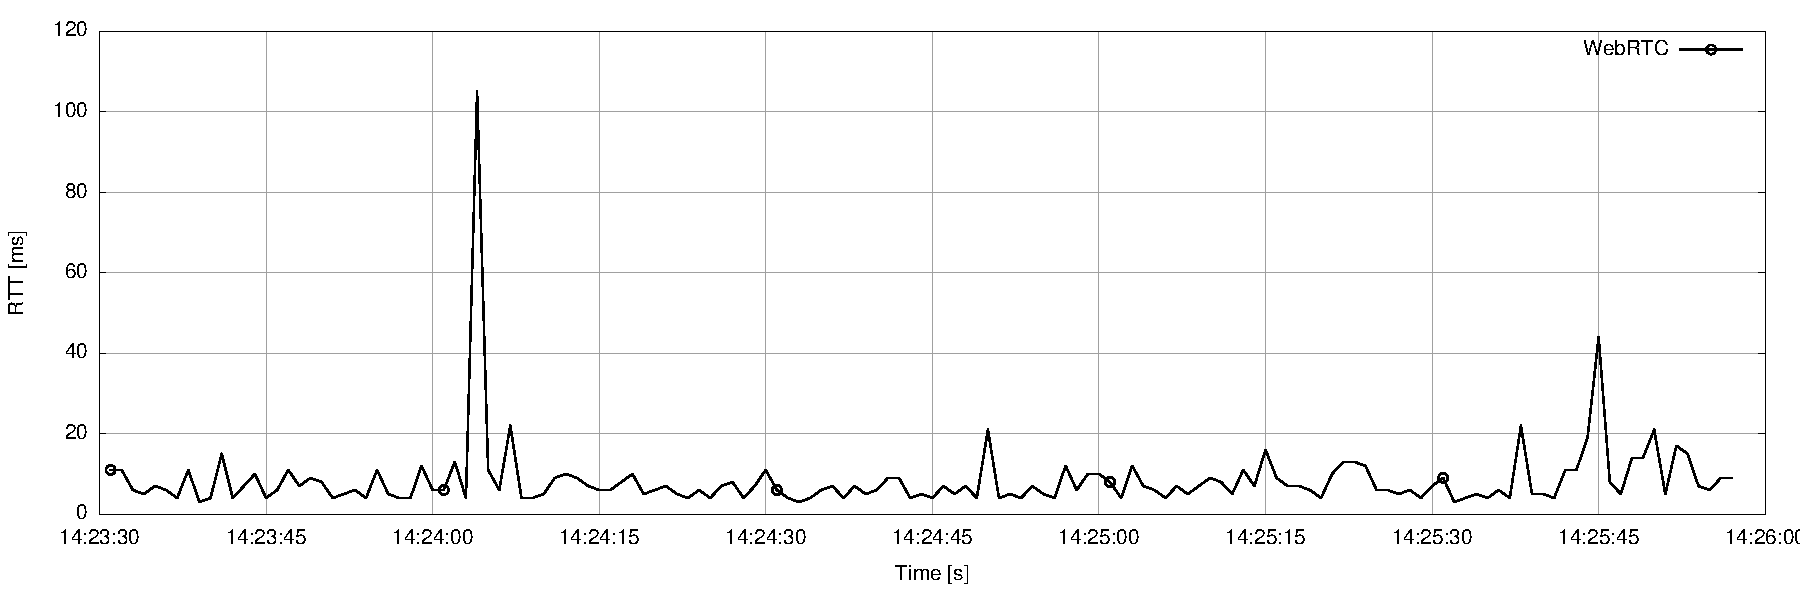
\includegraphics[width=1\textwidth]{./figures/p2prttexample.pdf}
      \caption[Point-to-point WebRTC RTT measure using Stats API over public WiFi]{Point-to-point WebRTC RTT measure using Stats API over public WiFi.}
	\label{fig:p2prttexample}
\end{figure}

Our Stats API also provides extra information such as RTT and loss rate, RTT should be provided natively by the WebRTC method but it is possible to calculate it by using the DataChannel provided by the PeerConnection, we are using this channel to send a UNIX TimeStamp object to the other peer and take it back, when the round trip is finished we compare it with the actual millisecond and obtain the total RTT.

Figure~\ref{fig:p2prttexample} represents the capture of a video call between two peers, if we are able to process the JavaScript forwarding function in an optimal way this would led to a precise RTT measurement hack without the need of Stats method.

\subsection{Connection Monitor}

Connection Monitor ({\it ConMon}) is a command line utility that relies on the transport layer and uses TCPDUMP to sniff all the packets that to go a certain interface and port~\cite{singhConMon}. This application is designed to specifically detect and capture RTP/UDP packets, relies on {\it libcap} for the capture in the network layer. This software detects and saves the header but discards the payload of the packet keeping the information we need for calculating our KPIs.

Typically we will run the PeerConnections between two devices and start capturing those packets by using {\it ConMon}. The PeerConnection will carry real data so the environment for testing will be a precise approach to a real scenario of WebRTC usage.

{\it ConMon} captures will be saved into different files and allow us to plot every stream bandwidth and calculate other parameters such as delay by using some parsing, this will allow us to compare how precise are both way of analyzing WebRTC as {\it ConMon} is working directly over the incoming interface and avoids all the processing that the browser is doing to send the stats to the JavaScript layer. Figure~\ref{fig:onetooneWifiRTCConMon} represents one video stream from the same call as Figure~\ref{fig:onetooneWifiRTC} and~\ref{fig:onetooneWifiRTCVideoStreams} but captured from the {\it ConMon} application.

 \begin{figure}[h]
  \centering
    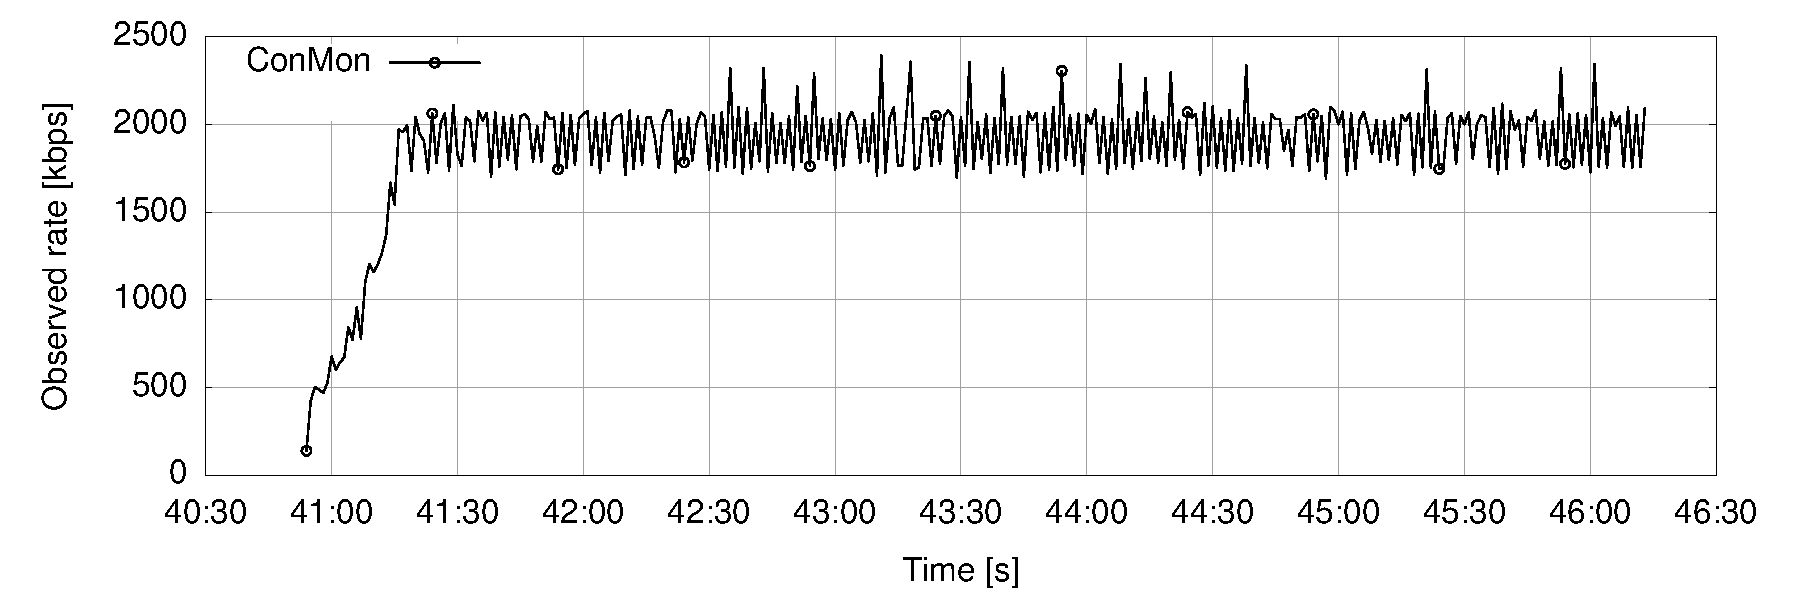
\includegraphics[width=1\textwidth]{./figures/onetooneWiFiConMon.pdf}
      \caption[Point-to-point WebRTC video stream throughput graph using ConMon over public WiFi]{Point-to-point WebRTC video stream throughput graph using ConMon over public WiFi.}
	\label{fig:onetooneWifiRTCConMon}
\end{figure}

The capture from {\it ConMon} will be very accurate capturing all the packets that go through the interface, dumping the values into the output file, this data will then be processed and averaged for every second prior plotting. This processing will lead to some fluctuations on the graph that distort the reality.

\subsection{Dummynet}

To check the performance of WebRTC we will need to modify the status of the network link. This is achieved using {\it Dummynet}, a command line network simulator that allow us to add bandwidth limitations, delays, packet losses and other distortions to the ongoing link.

{\it Dummynet} is an standard tool for some Linux distributions and OSX~\cite{dummynetTool}.

In order to get appropriate results with the constraints of the network we will have a machine acting as TURN for some tests, this machine will forward all the WebRTC traffic from one client to the other being transparent for both ends. The real goal of using TURN in WebRTC is to avoid and bypass some restrictive Firewalls that would block the connection, in our case, this works as a way to centralize the traffic flow through one path being able to be modified or tightened. From the performance perspective, when not adding any constraints to the TURN, the traffic and response is normal without the user noticing any difference.

Some problems arise when using {\it Dummynet} in our scenario, we will be using {\it VirtualBox} machines for some testing and to act as TURN, this means that there won't be real physical interfaces where {\it Dummynet} will be working on top. The accuracy of an emulator is given by the level of detail in the model of the system and how closely the hardware and software can reproduce the timing computed by the model~\cite{dummynetRevisited}. Considering that we are using standard Ubuntu images for our virtual machines we will need to modify the internal timer resolution of the kernel in order to get a closer approximation to reality, the default timer in a Linux kernel greater than 2.6.13 is 250Hz~\cite{linuxKernelTime}, this value must be changed to 1000Hz in all machines that we intend to run {\it Dummynet}. The change of timing for the kernel requires a full recompile of itself. This change will reduce the timing error from 4ms (default) to 1ms.

\subsection{Analysis of tools}

Both tools will be measuring the same metrics but from different OS layers, this provides us some extra data to be considered in order to see how the our Stats API work and if it is possible to implement some extra features relying on that data for the WebRTC API.

Because of the period needed to measure the results it is possible to have strange behaviors when plotting the results as the information regarding to the next data period can be considered as the previous one. This is an accuracy problem that cannot be approached easily, when looking at the graph is important to see if both peaks (positive and negative) get compensated as this would mean that the data has not been allocated to the current period. This accuracy error is a problem that can be observed when comparing both {\it ConMon} and Stats API capture as the browser will take some time to process the stats and send them to the JavaScript method, this will led to some extra error.

Figure~\ref{fig:p2pincommingStatsConmonWifi} and~\ref{fig:p2poutgoingStatsConmonWifi} plot two video streams being captured from Stats API and {\it ConMon}.

\begin{figure}[h]
	\begin{minipage}{.5\textwidth}
		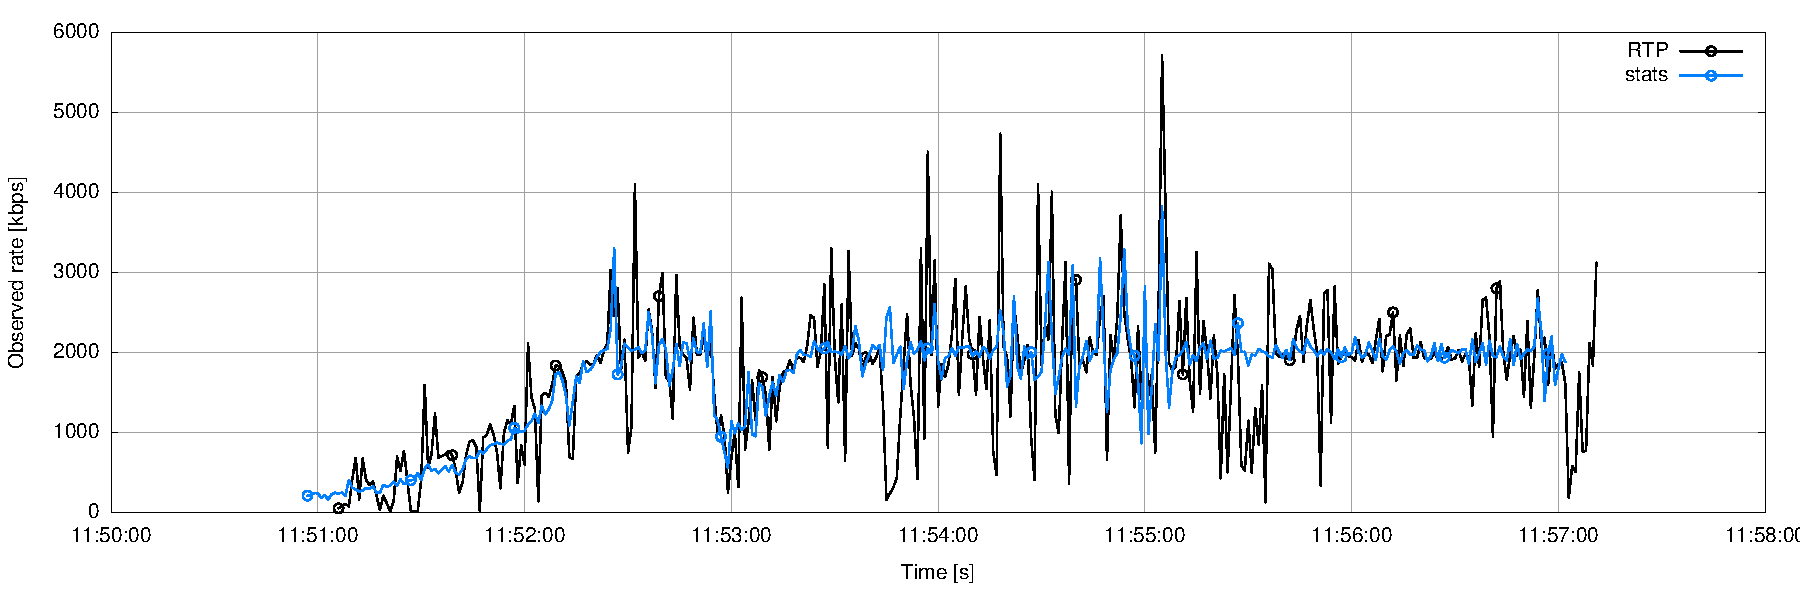
\includegraphics[width=1\textwidth]{./figures/p2pincommingStatsConmonWifi.pdf}
			\caption[P2P incoming video stream comparison between ConMon and Stats API over public WiFi]{P2P incoming video stream comparison between ConMon and Stats API over public WiFi.}
			\label{fig:p2pincommingStatsConmonWifi}
	 \end{minipage}
	 \begin{minipage}{.5\textwidth}
		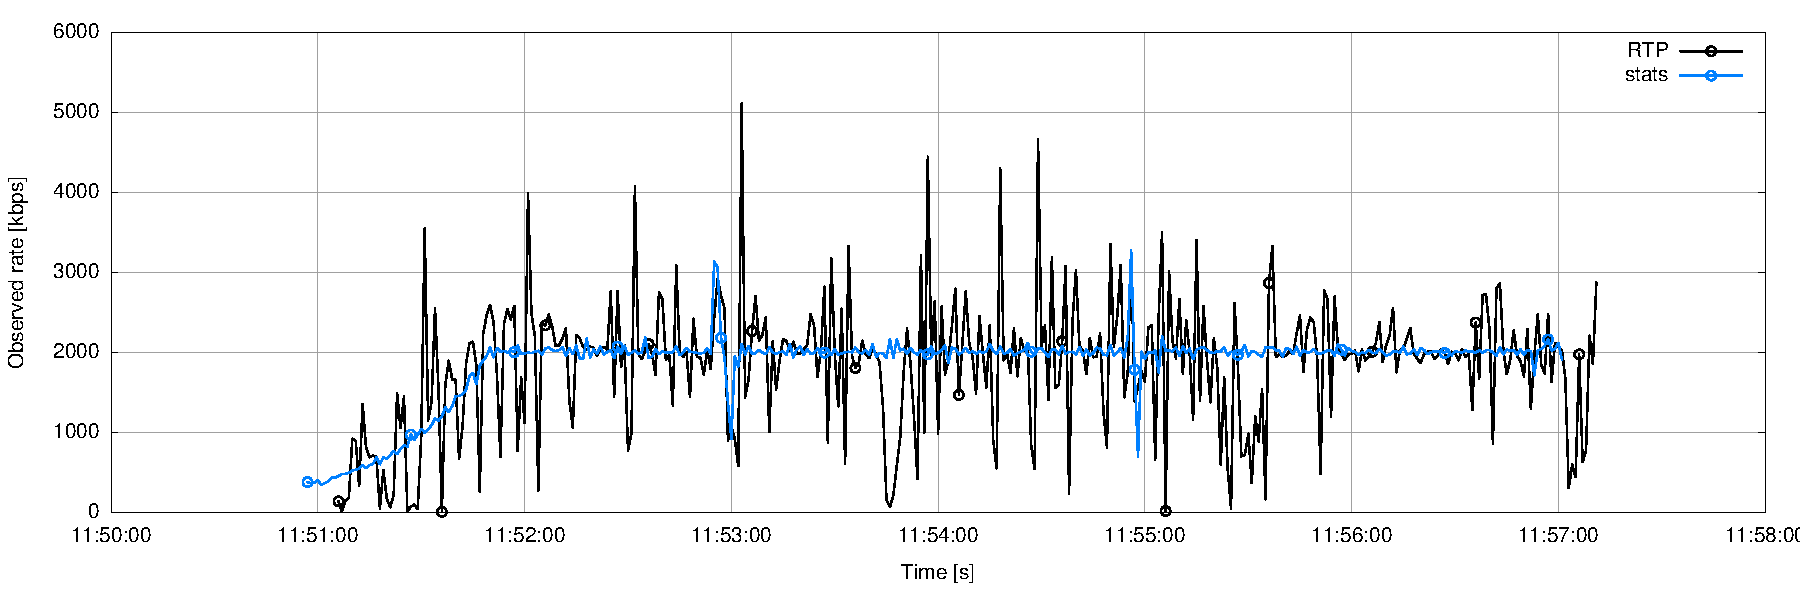
\includegraphics[width=1\textwidth]{./figures/p2poutgoingStatsConmonWifi.pdf}
			\caption[P2P outgoing video stream comparison between ConMon and Stats API over public WiFi]{P2P outgoing video stream comparison between ConMon and Stats API over public WiFi.}
			\label{fig:p2poutgoingStatsConmonWifi}
	 \end{minipage}
\end{figure}

Figure~\ref{fig:p2pincommingStatsConmonWifi} represents the incoming media stream from the other peer, this is why the throughput seems to be so unstable in some parts of the call, consider also that this test was performed using wireless connection without any network conditioner. In Figure~\ref{fig:p2poutgoingStatsConmonWifi} local stream is sent from the peer capturing with {\it ConMon} to the remote peer, the throughput captured using Stats API will be much more stable around the 2000 Kbps.

\subsection{Manual and automated testing}

For our testing scenario we consider two options, manual and automated testing. The first test environment does not give as much accuracy due to the impossibility to iterate the test many times in a controlled environment, if the second option is available the results can be compared after running the test for many iterations, this is much more accurate.

When considering both, the media being sent becomes a problem as there should be rich enough to be able to replicate a real call scenario. Google Chrome provides a fake video that can be activated by adding {\it --use-fake-device-for-media-stream} parameter, this video though might be too simple for our purposes.

%\begin{figure}[h]
%	\begin{minipage}{.5\textwidth}
%		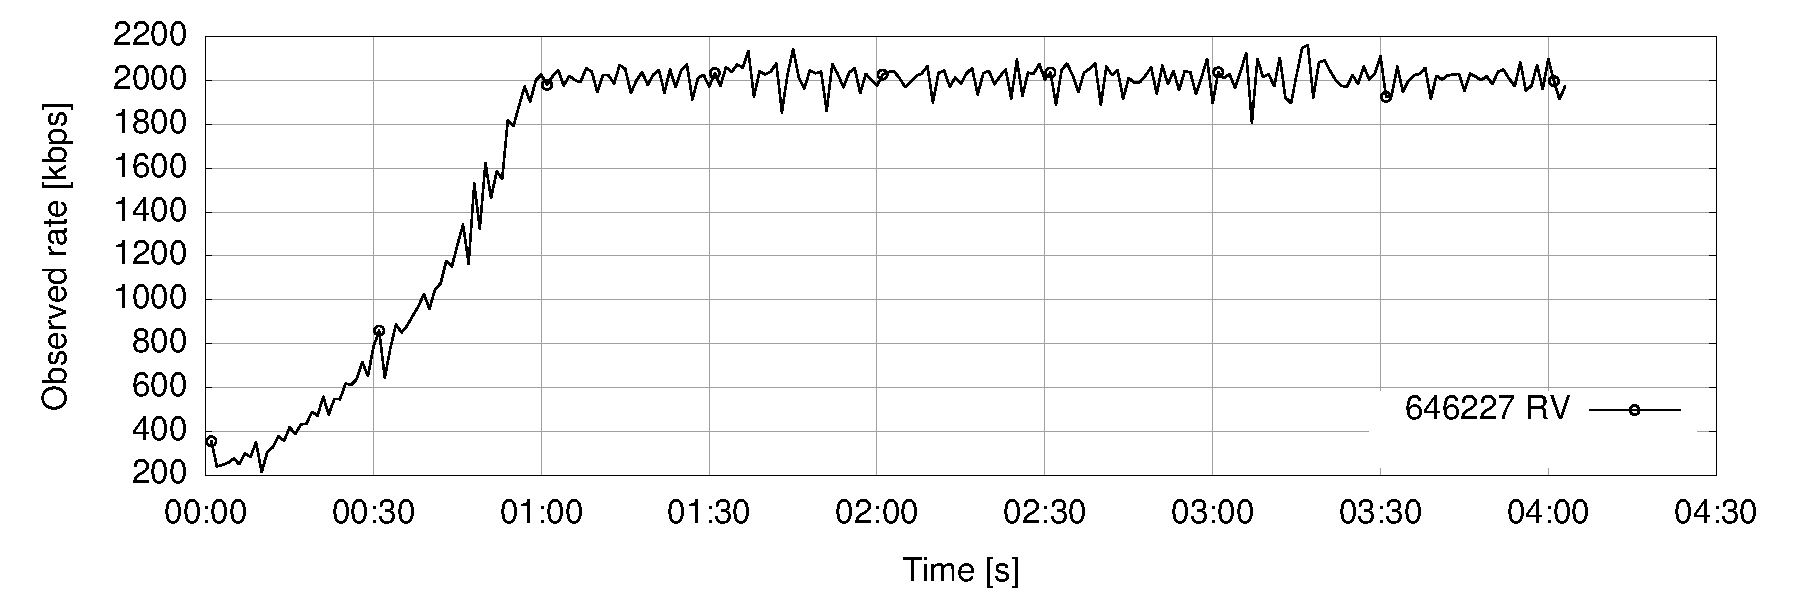
\includegraphics[width=1\textwidth]{./figures/realVideoChrome.pdf}
%			\caption[Video stream bandwidth between two peers using webcam]{Video call bandwidth between two peers using webcam.}
%			\label{fig:realVideoChrome}
%	 \end{minipage}
%	 \begin{minipage}{.5\textwidth}
%		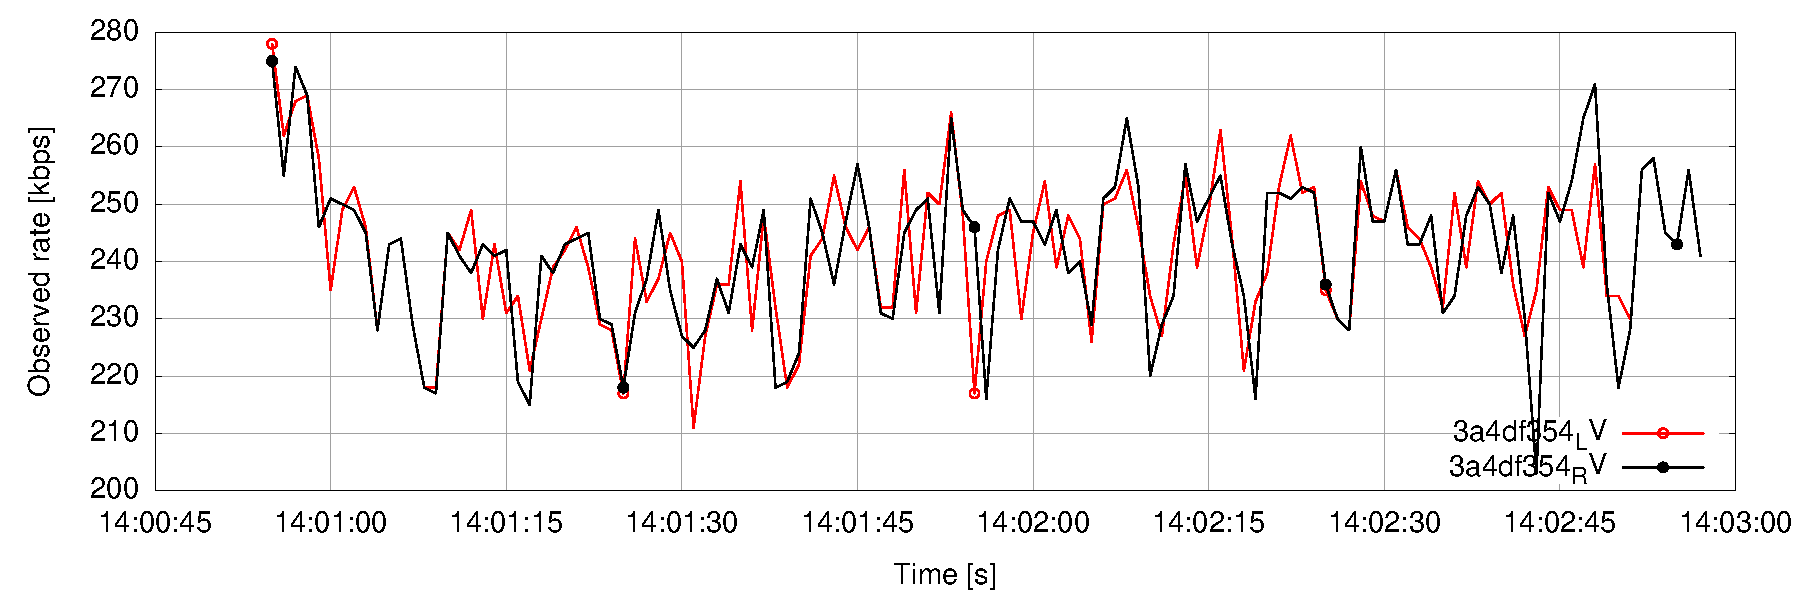
\includegraphics[width=1\textwidth]{./figures/automatedVideoChrome.pdf}
%			\caption[Video stream bandwidth between two peers using fake video]{Video stream bandwidth between two peers using fake video.}
%			\label{fig:automatedVideoChrome}
%	 \end{minipage}
%\end{figure}

 \begin{figure}[h]
  \centering
   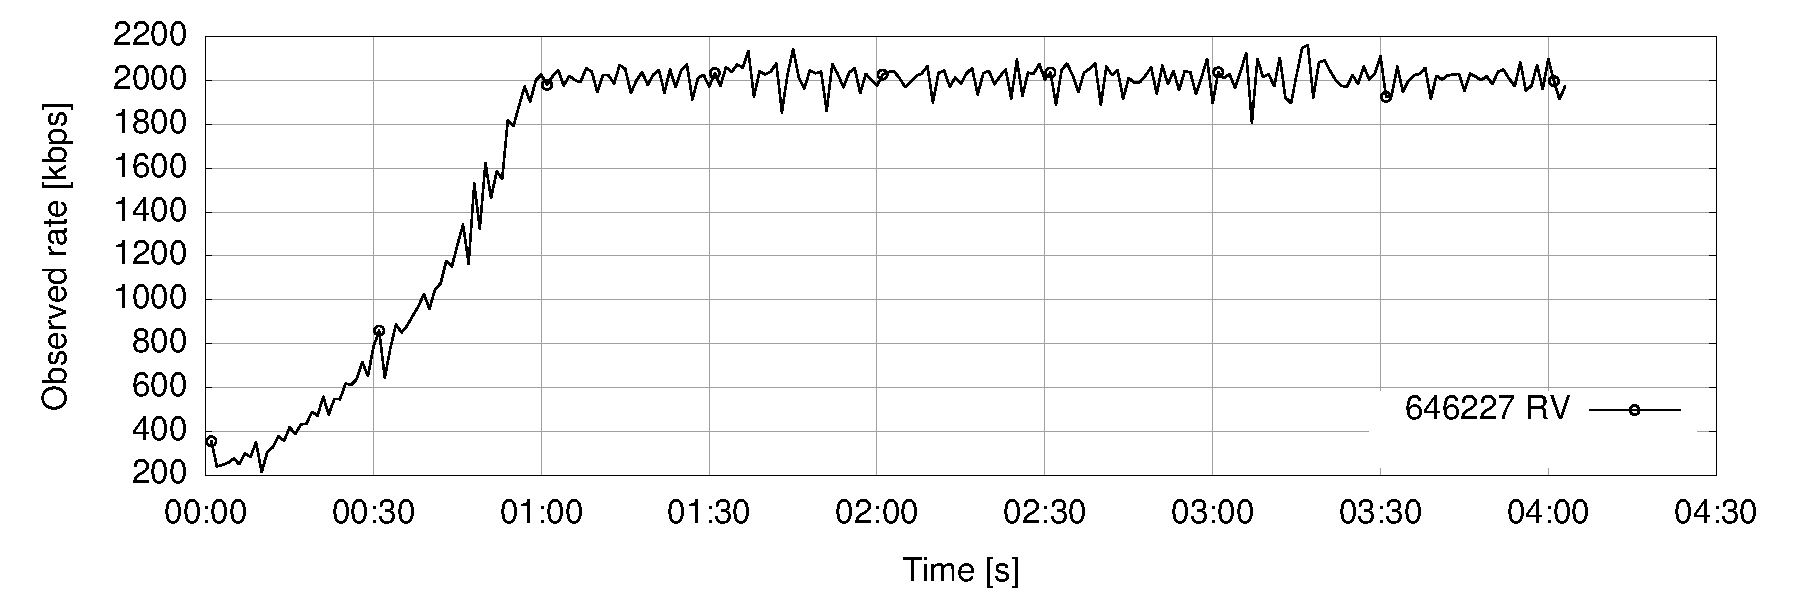
\includegraphics[width=1\textwidth]{./figures/realVideoChrome.pdf}
     \caption[Video stream bandwidth using webcam]{Video stream bandwidth using webcam input.}
	\label{fig:realVideoChrome}
%\end{figure}
 %\begin{figure}[h]
  \centering
	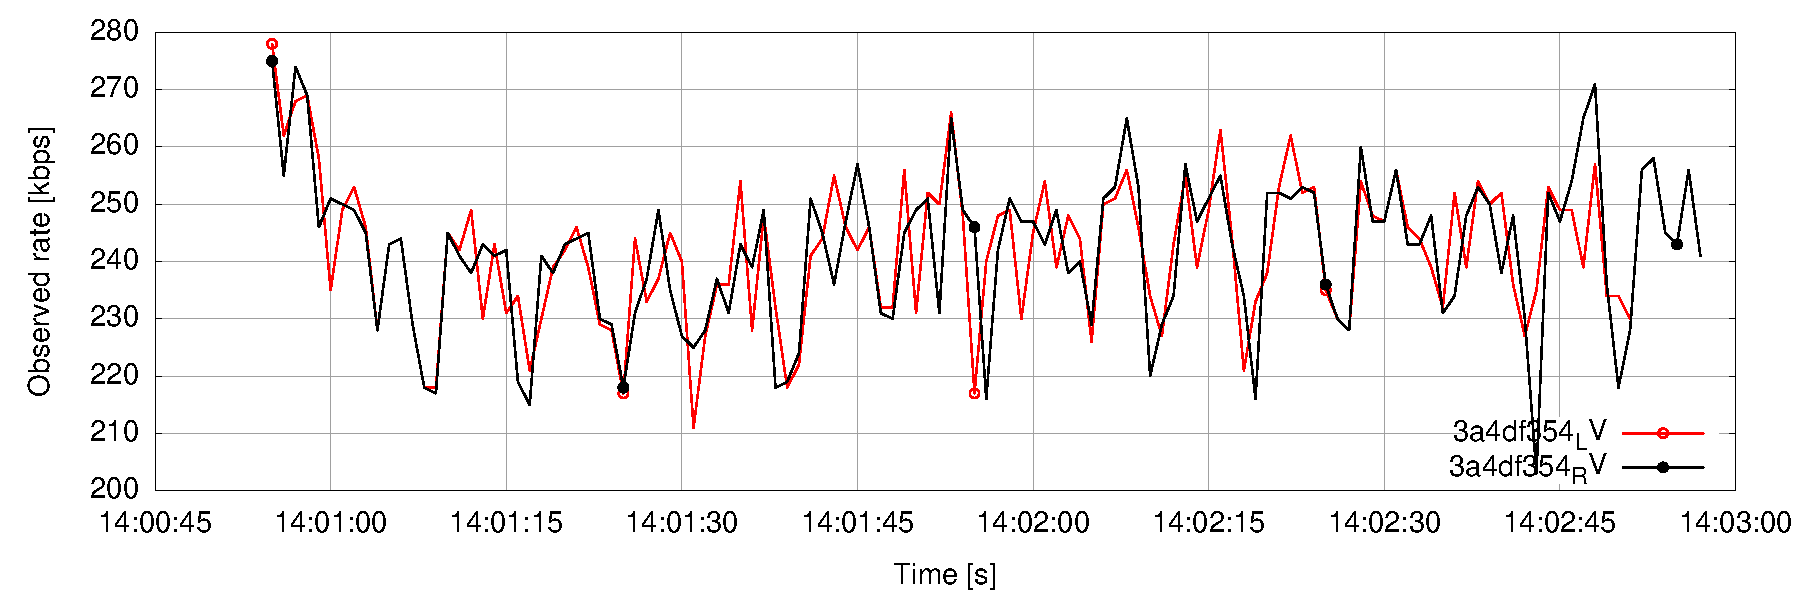
\includegraphics[width=1\textwidth]{./figures/automatedVideoChrome.pdf}
	\caption[Video stream bandwidth using Chrome default fake content]{Video stream bandwidth using Chrome default fake video input.}
	\label{fig:automatedVideoChrome}
\end{figure}

Figure~\ref{fig:realVideoChrome} represents the bandwidth that a real video call uses when sending the stream to the other peer, that capture shows the same stream from the origin an remote {\it StatsAPI} perspective. The bandwidth allocated goes up to 2000 Kbps. On the other hand, Figure~\ref{fig:automatedVideoChrome} represents the same call by using the built-in fake video on both clients, the bandwidth in this case drops to an average of 250 Kbps. Those figures represent the same stream identified with the SSRC that corresponds, input from receiver and output from origin, this representation helps us to identify any possible distortion on the link. Google Chrome uses a bitmap system to draw the figures and components to be rendered in the video tag, this means that the amount of encoding and bandwidth used is low compared to a real webcam.

To address this issue in the video streamed from our automated devices we have built a fake input device on the virtual machines, procedure is described in Appendix~\ref{sec:fakeVideo}.

 \begin{figure}[h]
  \centering
    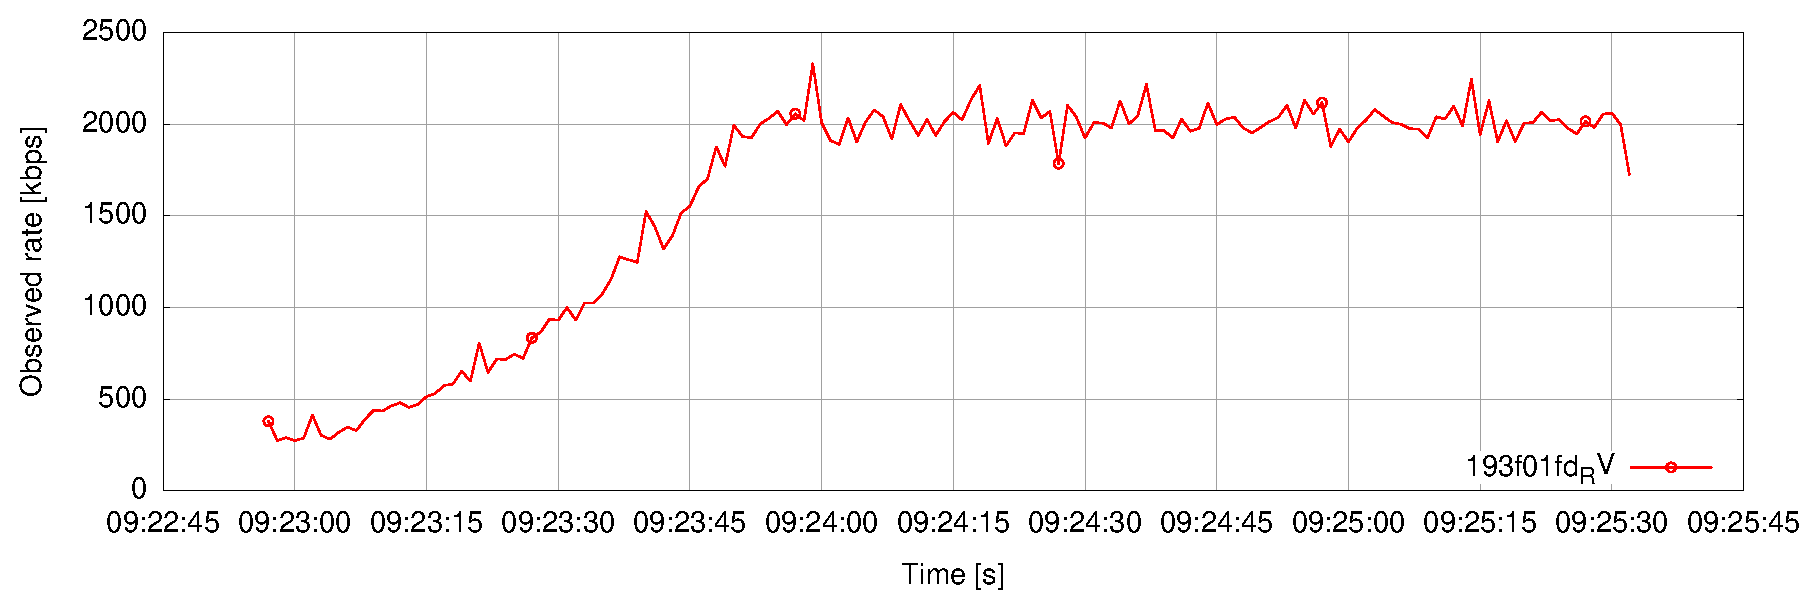
\includegraphics[width=1\textwidth]{./figures/testV4L2niklas.pdf}
      \caption[Video stream bandwidth using V4L2Loopback fake YUV file]{Video stream bandwidth using V4L2Loopback fake YUV file.}
	\label{fig:testV4L2niklas}
\end{figure}

Figure~\ref{fig:testV4L2niklas} shows the bandwidth of a video stream measured by our {\it Stats API} using an YUV video captured from a Logitech HD Pro C910 as source, resolution is 640x480 at a frame-rate of 30 fps. Results show an approximate average bandwidth of 2000 Kbps which is a realistic approach to a real webcam. This setup will allow us to run multiple tests without the need of a webcam.

%Tests
\section{Testing WebRTC}

\thispagestyle{empty}

In this chapter we will study how WebRTC performs in different use cases and topologies previously described in chapter~\ref{sec:topologies}. All tests will be done using a real working environment with the tools previously mentioned in chapter~\ref{sec:testingEnv}.

\subsection{Point-to-point}

In a point-to-point scenario we have performed different tests to calculate how the application performs. 

\subsubsection{WiFi scenario}

Firstly we have stablished a simple call between two peers that handle video and audio in an open WiFi network. This network does not carry any UDP packet filter or Firewall, the connection is performed without the need of STUN or TURN, we could easily say it is a straight forward peer-to-peer connection. The aim of this test is to observe how the captures differ between origin and receiver on the {\it StatsAPI} and {\it ConMon} layer.

 \begin{figure}[h]
  \centering
    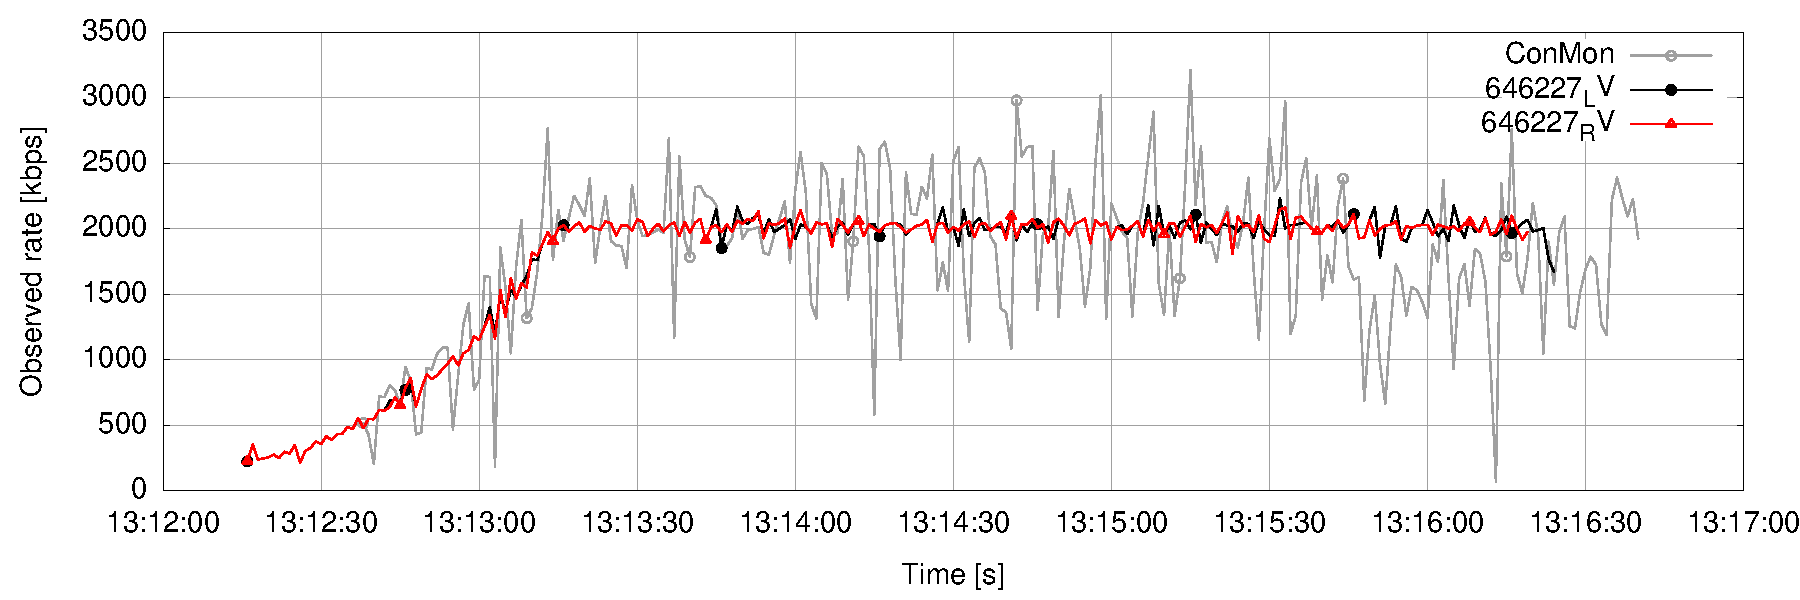
\includegraphics[width=1\textwidth]{./figures/onetoone_wifi_statsconmon.pdf}
      \caption[Point-to-point video stream plot using StatsAPI and ConMon data over WiFi]{Point-to-point video stream plot using StatsAPI and ConMon data over WiFi.}
	\label{fig:onetooneWifistatsconmon}
\end{figure}

Figure~\ref{fig:onetooneWifistatsconmon} represents the throughput rate on the same video stream, the three lines are the comparison between local video stream in origin peer, remote video stream in receiver peer and {\it ConMon} capture of the remote video stream on the receiver peer. All three streams contain the same data but they are measured in different layers, this will help us to understand the difference of throughput that is handling the overhead of the RTP and the disruption caused by the WiFi network.

Notice that red and black colors represent the Local Video (LV) and Remote Video (RV) from the same SSRC, both captures indicate the same stream captured using {\it StatsAPI}, and the grey line plots the capture performed using {\it ConMon} of the same SSRC. It is easy to observe that both {\it StatsAPI} captures are similar, some offset is produced due to the processing time between the network layer and the browser API that returns all values. Besides this, the capture is neat and throughput at the output of the origin client and input of the receiver is similar. Capture in the network layer is more abrupt as all packets are captured and the period of calculus when plotting affects when the value is added, when having two opposite values peaks they should be balanced, meaning that the transmission in most of the period is stable and the peaks when plotting are a result of accuracy. Call duration in this test has been around five minutes. Some areas, mostly between 13.15.30 and 13.16.00, show a strange behavior of the link that might be produced by the WiFi, this throughput distortion is balanced on the WebRTC layer as the throughput delivered by the API does not change.

When we try to measure the quality of the call one important indicator is the delay, to calculate the delay we can either use the RTT measured by our {\it StatsAPI} or use the captures performed on the network layer by {\it ConMon}. The {\it ConMon} procedure will give us a high accuracy on the delay subtracting both timestamps from both of the clients, this will require to reduce the drift of the internal clock of the computers.

 \begin{figure}[h]
  \centering
    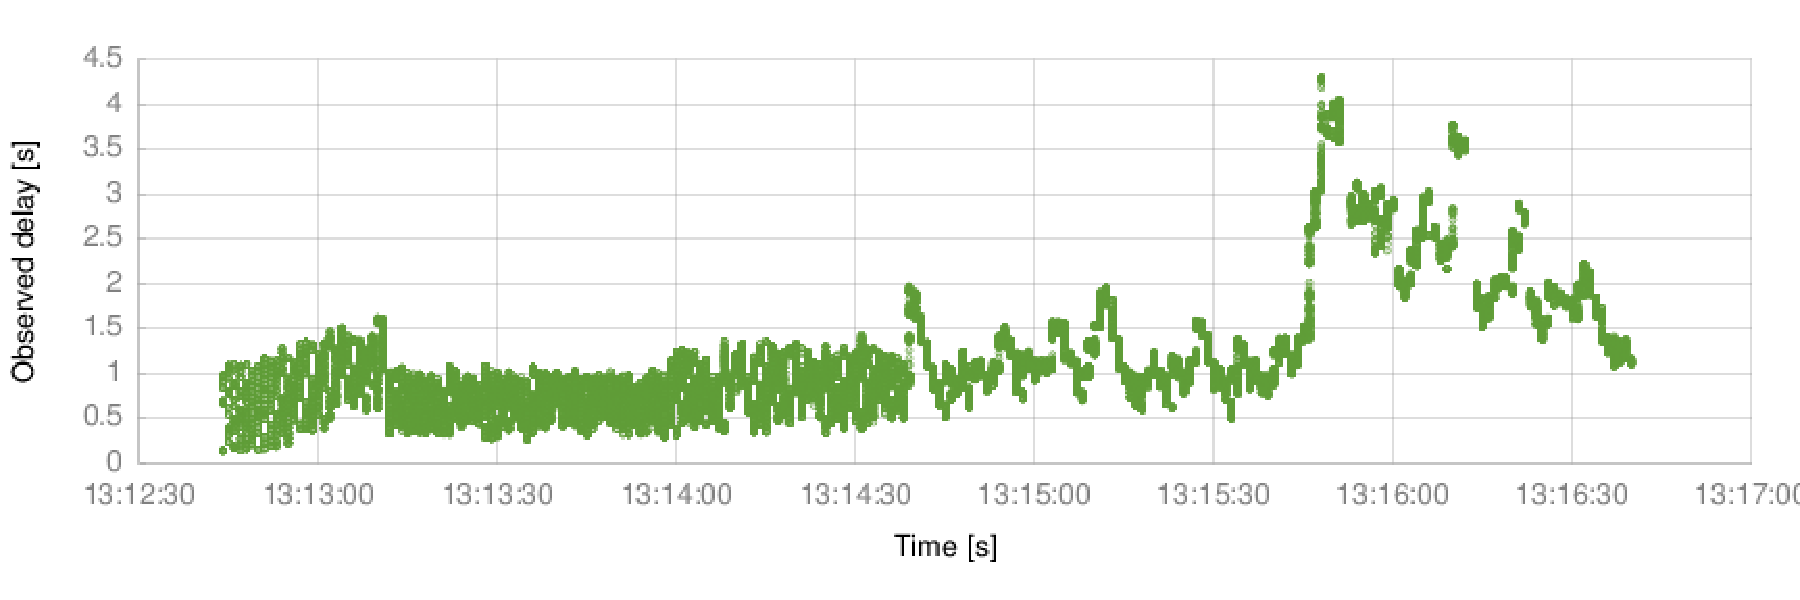
\includegraphics[width=1\textwidth]{./figures/delay_116_646227.pdf}
      \caption[Delay calculated on the same stream captured using ConMon in both ends over WiFi]{Delay calculated on the same stream captured using ConMon in both ends over WiFi.}
	\label{fig:delay_116_646227}
\end{figure}

Figure~\ref{fig:delay_116_646227} represents the delay of the stream plotted in~\ref{fig:onetooneWifistatsconmon}. We can see that the quality of the call is affected by the network distortion at the end of Figure~\ref{fig:onetooneWifistatsconmon}, this variation of the throughput delivers a high delay of more than 4 seconds during some period of time between 13:15:30 and 13:16:30, the media received at that time will not render correctly and the user experience of the call is going to be worst than at the beginning of the call. A bursty WiFi network will led to delay even the bandwidth seems to be stable.

\subsubsection{Non-constrained link test}

After seeing how WebRTC performs in WiFi  we are going to proceed with all tests in a controlled wired scenario adding different constraints to the link. This tests will be automated running ten iterations every time in order to get as much accurate results as possible.
 
 \begin{figure}[h]
  \centering
    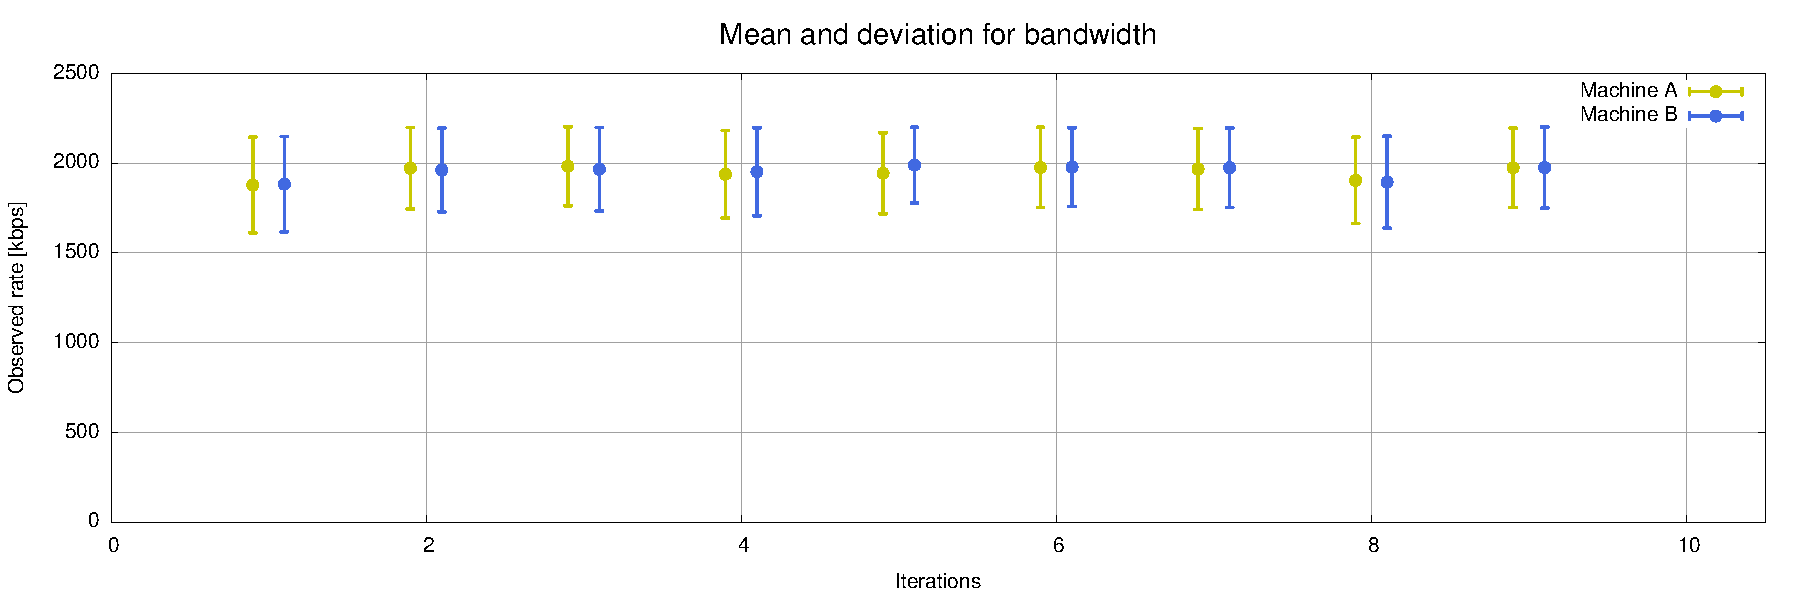
\includegraphics[width=1\textwidth]{./figures/no_ipfw.pdf}
      \caption[Bandwidth results for non-conditioned link]{Bandwidth results for non-conditioned link.}
	\label{fig:no_ipfw}
\end{figure}

Figure~\ref{fig:no_ipfw} plots the average bandwidth of every call in a wired network without any link condition, the average bandwidth obtained in the test is 1949.7 Kbit/s with 233 Kbit/s of deviation which gives the conclusion of having approximately 1 Mbit/s standard bandwidth in a video stream for a non-conditioned link in WebRTC. Delay result in 5.1 ms with 1.5 ms deviation and RTT about 9.5 ms. Those results can be taken as standard for a non-conditioned WebRTC with high bandwidth resources. A summary of results is shown in Table~\ref{fig:p2p_no_ipfw}. Some interesting results to track is the amount of calls failed in every test, considering all those calls go through a TURN server we might be able to approximate the success rate when establishing calls. All results go along with the deviation being this an important factor, in this test without any link conditioner we might have small deviation values such as milliseconds, but when adding conditions to the link those values will grow carrying less accuracy.
Setup time is stablished as the time it take since the start of the PeerConnection object until the media stream from the other peer arrives, this value directly affects the time it takes for a user to be able to start talking, in the optimal environment it takes about 1.5 seconds to start the call. We also had zero packet losses and two calls that failed to succeed using TURN in the standard environment.

\begin{table}[h]
\begin{center}
    \begin{tabular}{c D{,}{\pm}{-1} D{,}{\pm}{-1} D{,}{\pm}{-1} }
   	 \toprule
	\textit{}
	& \multicolumn{1}{c}{\textit{Machine A}}
	& \multicolumn{1}{c}{\textit{Machine B}}
	& \multicolumn{1}{c}{\textit{Overall}}\\
	\midrule
	\textbf{CPU (\%)} & 48.76 ,2.76 & 48.83 ,2.78 & 48.79 ,2.77\\
	\textbf{Memory (\%)} & 35.98 ,0.3 & 36.43 ,0.29 & 36.21 ,0.29\\
	\textbf{Bandwidth (Kbit/s)} & 1947.61 ,232.75 & 1951.76 ,234.5 & 1949.7 ,233.62\\
	\textbf{Setup time (ms)} & 1436.33 ,25 & 1447.44 ,22.71 & 1441.88 ,24.04\\
	\textbf{RTT (ms)} & 9.49 ,2.11 & 9.64 ,2.71 & 9.57 ,2.41\\
	\textbf{Delay (ms)} & 4.84 ,1.5 & 5.4 ,1.53 & 5.12 ,1.52\\
	\bottomrule
    \end{tabular}
    \caption[P2P test with no link conditions]{P2P test with no link conditions.}
    \label{fig:p2p_no_ipfw}
\end{center}
\end{table}

Delay values in Table~\ref{fig:p2p_no_ipfw} are represented as a mean calculation of all the delay obtained in the link, thus this value is not representative of what happened in the call. Considering the example in Figure~\ref{fig:delay_116_646227} we can see that the delay can variate during the call being the mean not appropriate to measure the response against the conditions of the link. In order to observe the behavior of WebRTC in delay we have two different approaches, the mean delay with deviation and delay distribution of all calls. 

 \begin{figure}[h]
  \centering
    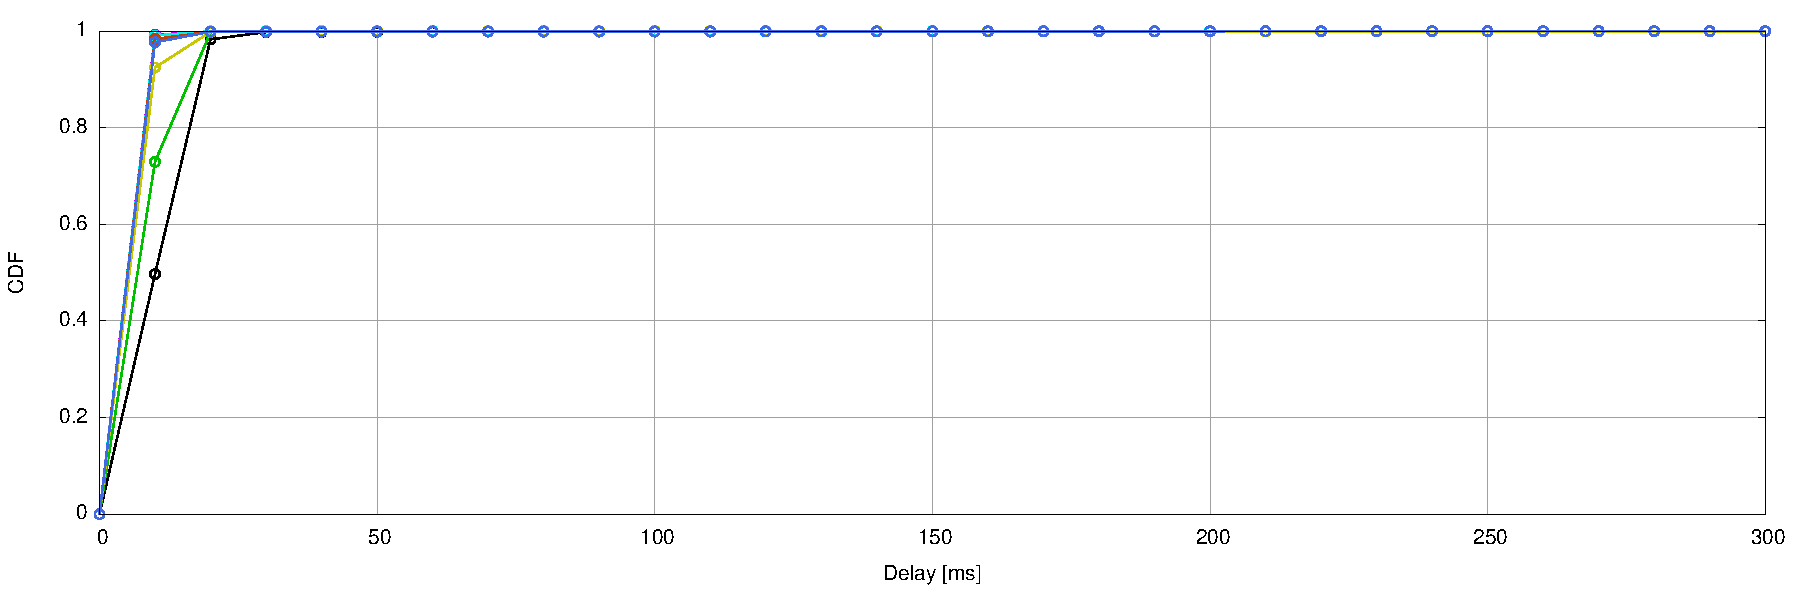
\includegraphics[width=1\textwidth]{./figures/total_delay_distribution_no_ipfw.pdf}
      \caption[Delay distribution in each P2P iterations with no link constraints]{Delay distribution in each P2P iterations with no link constraints.}
	\label{fig:total_delay_distribution_no_ipfw}
\end{figure}

 \begin{figure}[h]
  \centering
    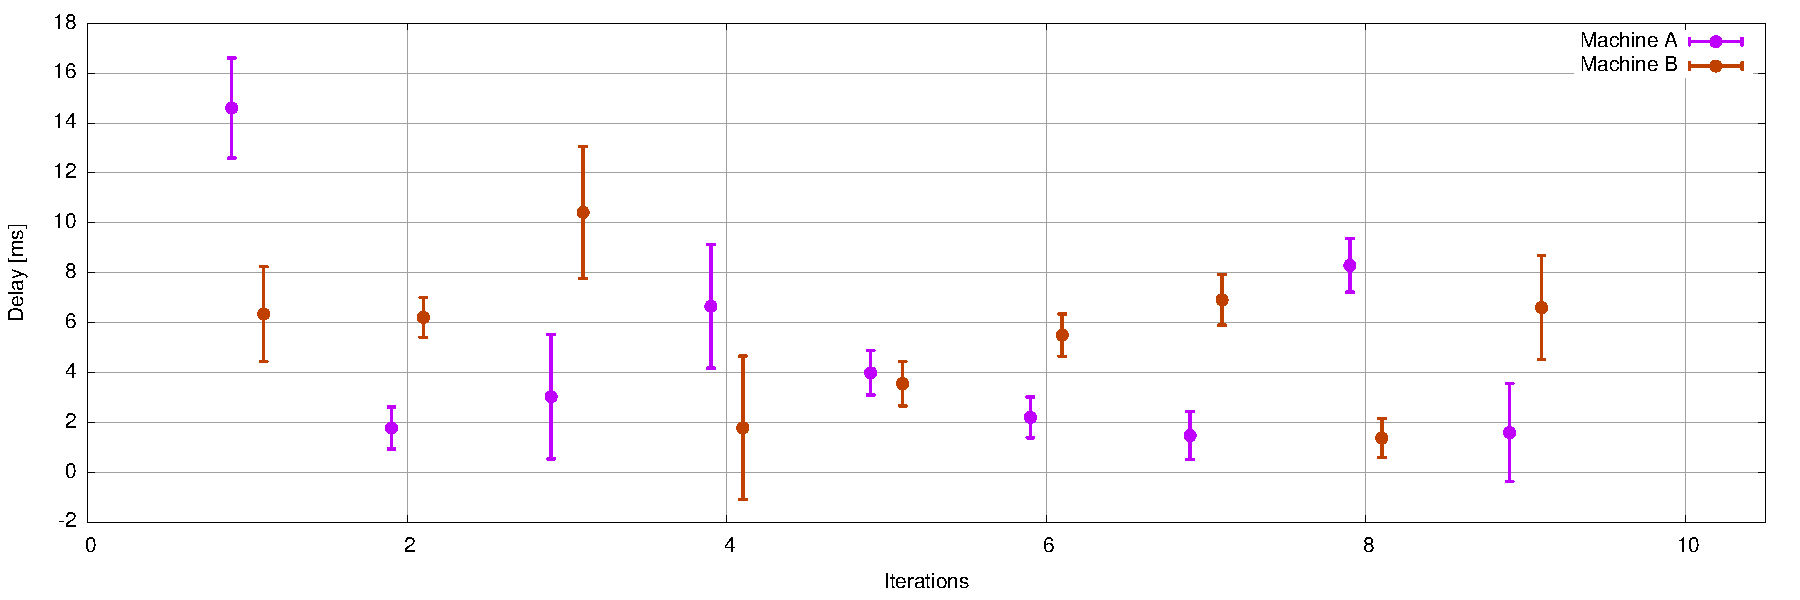
\includegraphics[width=1\textwidth]{./figures/mean_deviation_delay_no_ipfw.pdf}
      \caption[Bandwidth mean and deviation for delay in each P2P iterations with no link constraints]{Mean and deviation for delay in each P2P iterations with no link constraints.}
	\label{fig:mean_deviation_delay_no_ipfw}
\end{figure}

Figure~\ref{fig:mean_deviation_delay_no_ipfw} represents the mean and deviation of delay calculated for all iterations, this delay is calculated on basis with the arrival timestamp for each packet with the captures performed in both sides by {\it ConMon}. We run an NTPD daemon to calculate the drift on the time and sync both machines.  There is small amount of drift of maximum 3ms in the worst case and as small as 1ms in the best one. In Figure~\ref{fig:total_delay_distribution_no_ipfw}, the distribution is given by the amount of packets that have some specific amount of delay, they are counted by batches of 10ms with a maximum range of 300ms. Most of the packets run with less than 25ms delay in all the iterations. The user experience with this small amount of delay with no aggressive steps in the plot will be barely negligible. Figures~\ref{fig:mean_deviation_delay_no_ipfw} and~\ref{fig:total_delay_distribution_no_ipfw} differentiate from Figure~\ref{fig:delay_116_646227} in the measurement of a global delay for an specific constraint scenario instead of just plotting a single call case, many aspects may affect the delay and the an optimal way to observe it is to plot the distribution and deviation of each iteration and try to guess a patron that repeats, Figure~\ref{fig:delay_116_646227} is good to observe just one call if we add some conditions to the link meanwhile the call is going on.

\subsubsection{Behavior in lossy environments}

We have performed some tests regarding lossy environments to see how WebRTC behaves in those, lossy situations can be given with some mobile environments with low coverage or just by having a busy link with no resources available.

We have tested the topology with 1, 5, 10 and 20\% of packet loss, according to the results in Table~\ref{fig:p2p_packet_bw} we are seeing a pretty good response from the internal algorithm up to 5\% with small effect to the bandwidth and delay. When running with 10\% loss the bandwidth drops to an average of 1140.8 Kbit/s and 162 Kbit/s deviation which is half of the corresponding amount for an standard call, this affects the quality of the link and video, 20\% loss will affect to the performance dropping the bandwidth to an average of 314.4 Kbit/s with 62 Kbit/s deviation. We can say that the video quality will be worst with lossy networks but the delay is not affected, having a delay distribution response that matches the standard case without affecting the way users will talk, quality will be worst but the call will be correct in terms of usage. All metrics are in the normal range except bandwidth.

The algorithm used in WebRTC regarding to packet loss is proven to work fine in lossy environments with the results obtained, but there is a big gap of performance in the 10\% loss network compared to the results with 20\%, it is obviously a big amount of packets but the response with 20\% is significantly better than the one with 10\%.

\begin{table}[h]
\begin{center}
    \begin{tabular}{c D{,}{\pm}{-1} D{,}{\pm}{-1} D{,}{\pm}{-1} }
   	 \toprule
	\textit{}
	& \multicolumn{1}{c}{\textit{Machine A}}
	& \multicolumn{1}{c}{\textit{Machine B}}
	& \multicolumn{1}{c}{\textit{Overall}}\\
	\midrule
	\textbf{1\% (Kbit/s)} & 1913.59 ,252.11 & 1880.24 ,261.46 & 1896.91 ,256.78\\
	\textbf{5\% (Kbit/s)} & 1609.65 ,158.46 & 1527.84 ,198.59 & 1568.74  ,178.52\\
	\textbf{10\% (Kbit/s)} & 1166.70 ,145.96 & 1114.94 ,177.88 & 1140.82 ,161.92\\
	\textbf{20\% (Kbit/s)} & 333.34 ,65.99 & 295.46 ,57.98 & 314.4 ,61.98\\
	\bottomrule
    \end{tabular}
    \caption[Averaged bandwidth with different packet loss conditions]{Averaged bandwidth with different packet loss conditions.}
    \label{fig:p2p_packet_bw}
\end{center}
\end{table}

The amount of packets lost in every test is slightly lower than the exact percentage of loss because the use of Forward Error Correction in WebRTC in Chrome, this mechanism is used to control errors in data connection with noisy channels that led to packet losses. FEC is not a must feature to implement in WebRTC but Chrome carries it as default.

When using FEC the sender encodes the message in a redundant way, by having this redundancy the receiver is able to detect a limited number of errors and autocorrect those errors without requiring retransmission.

On the other side, the sender calculates its rate based on the receive report that arrives from the receiver, if this report is not received within two times the maximum interval WebRTC congestion mechanism will consider that all packets during that period have been lost halving the rate in the sender. In order to improve response in lossy environments we could consider calculating the optimal value for this interval considering all the possible situations. Considering the congestion algorithm in WebRTC~\cite{alvestrandCongestion2012}, the rate should not vary when having between 2-10\% of packet losses. Table~\ref{fig:p2p_packet_bw} proves that this mechanism is not working properly as we are noticing reduction of rate with 5\% of packet losses, the mechanism should start modifying the rate above 10\% of packet lost calculating a new sender available bandwidth (A$_{\textrm{s}}$) using Equation~\ref{eq:RateCalc} being {\it p} the packet loss ratio.

\begin{equation}
	A_s ( i ) = A_s ( i - 1 ) \times (1 - \frac{p}{2}) 
	\label{eq:RateCalc}
\end{equation}

If the packet loss is less than 2\% the increase of bandwidth will be given by Equation~\ref{eq:RateCalc2}.

\begin{equation}
	A_s ( i ) = 1.05 \times (A_s ( i - 1 ) + 1000) 
	\label{eq:RateCalc2}
\end{equation}

\subsubsection{Delayed networks}

Another interesting situation that are given in mobile environments and queued networks is delay, we have also tested the performance of WebRTC in those conditions. We have benchmarked tests in different one-way delays, 50, 100, 200 and 500ms. In our case, the RTT results should be multiplied by two.

Delay modeling for real time applications is difficult and can be done using the timestamp of the incoming packets, the incoming frame will be delayed if the arrival time difference is larger than the timestamp difference compared to its predecessor frame.

We have noticed that the system performs badly when having even small delays up to 100ms. The response of WebRTC is to reduce the bandwidth by discarding packets, this means that the congestion control systems that act in those environments are not working correctly. On the other hand, delay output does behave correctly having a continuous delay of the according time configured in the constraints, there are no sudden increases of delay and the deviation in delay fits in the standard limits.

Table~\ref{fig:p2p_delay_bw} represents the bandwidth response to the delay conditions, it is interesting to see that the deviation with the biggest delay is smaller than expected. Only with 50ms the system will output a good quality call, when increasing delay the performance of the video will decrease. WebRTC uses VP8 codec which degrades gracefully the quality in packet loss and delay conditions but the response in this case should be better if the congestion mechanisms worked properly.

\begin{table}[h]
\begin{center}
    \begin{tabular}{c D{,}{\pm}{-1} D{,}{\pm}{-1} D{,}{\pm}{-1} }
   	 \toprule
	\textit{}
	& \multicolumn{1}{c}{\textit{Machine A}}
	& \multicolumn{1}{c}{\textit{Machine B}}
	& \multicolumn{1}{c}{\textit{Overall}}\\
	\midrule
	\textbf{50ms (Kbit/s)} & 1909.31 ,258.09 & 1917.81 ,251.62 & 1913.56 ,254.86\\
	\textbf{100ms (Kbit/s)} & 1516.07 ,263.43 & 1453.94 ,272.79 & 1485 ,268.11\\
	\textbf{200ms (Kbit/s)} & 503.71 ,116.45 & 617.92 ,142.69 & 560.82 ,129.57\\
	\textbf{500ms (Kbit/s)} & 303.58 ,59.22 & 207.77 ,32.48 & 255.67 ,45.85\\
	\bottomrule
    \end{tabular}
    \caption[Summary of averaged bandwidth with different delay conditions]{Summary of averaged bandwidth with different delay conditions.}
    \label{fig:p2p_delay_bw}
\end{center}
\end{table}

We can also observe that every iteration follows a different pattern even having an averaged result, Figure~\ref{fig:mean_deviation_bw_delay200} show the test performed at 200ms and the iterations that fail to keep a constant rate making the amount of artifacts in the video affect the quality of the call. We can certainly confirm that the methods that WebRTC should use to control the congestion in the call are not working as they should.

 \begin{figure}[h]
  \centering
    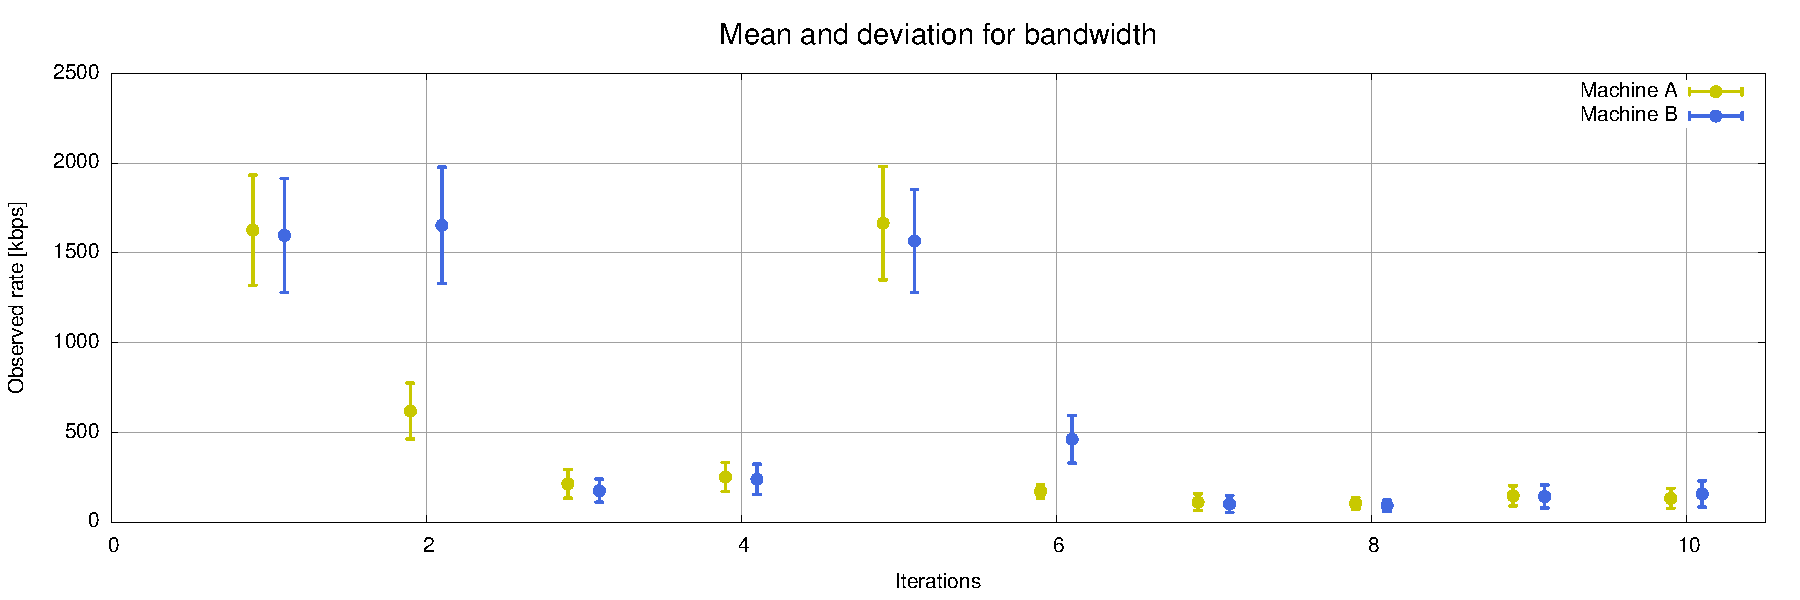
\includegraphics[width=1\textwidth]{./figures/mean_deviation_bw_delay200.pdf}
      \caption[Bandwidth mean and deviation for P2P 200 ms delay test]{Mean and deviation for P2P 200 ms delay test.}
	\label{fig:mean_deviation_bw_delay200}
\end{figure}

The problem with WebRTC relies in the usage of RTP over UDP for packet transport as UDP does not carry congestion control mechanisms that TCP does, when having real time media adapting the encoding to accommodate the varying bandwidth is difficult and cannot be done rapidly.

Low latency networks will play a big role when WebRTC extends to mobile devices and the ability to react properly to delays and packet losses will be crucial for the success of WebRTC in those environments against its competitors.

\subsubsection{Loss and delay}

Regarding P2P scenario we also tested the possibility of having a combined lossy network with delay added to it, this kind of environment could be easily found in mobile applications in low coverage areas. We have set 10\% packet loss with different delays such as 25ms, 50ms, 100ms and 200ms. In Table~\ref{fig:p2p_packet_bw} we saw an average of over 1 Mbit/s of bandwidth usage in 10\% loss environments, the result when adding delay to the constraint is  an average of barely 60 Kbit/s. Those results differ due to the difficulty of WebRTC to handle congestion in those environments. 

\begin{table}[h]
\begin{center}
    \begin{tabular}{c D{,}{\pm}{-1} D{,}{\pm}{-1} D{,}{\pm}{-1} }
   	 \toprule
	\textit{}
	& \multicolumn{1}{c}{\textit{Machine A}}
	& \multicolumn{1}{c}{\textit{Machine B}}
	& \multicolumn{1}{c}{\textit{Overall}}\\
	\midrule
	\textbf{25ms (Kbit/s)} & 72.59 ,18.54 & 70.69 ,18.09 & 71.78 ,18.32\\
	\textbf{50ms (Kbit/s)} & 59.7 ,16.84 & 60.36 ,18 & 60.03 ,17.42\\
	\textbf{100ms (Kbit/s)} & 63.3 ,19.29 & 64.82 ,20.95 & 64.06 ,20.12\\
	\textbf{200ms (Kbit/s)} & 66.89 ,20.12 & 65.66 ,19.63 & 66.27 ,19.87\\
	\bottomrule
    \end{tabular}
    \caption[Averaged bandwidth with different delay conditions with 10\% packet loss]{Averaged bandwidth with different delay conditions with 10\% packet loss.}
    \label{fig:p2p_delay_loss_bw}
\end{center}
\end{table}

Table~\ref{fig:p2p_delay_loss_bw} describes the averaged bandwidth result with not much difference in each situation.If we study the way WebRTC calculates the rate in difficult situations we can see that the sender will establish its decision on the RTT, packet loss and available bandwidth that is estimated from the receiving side using Equation~\ref{eq:RateCalc}~\cite{alvestrandCongestion2012}. Obviously the real output differs form the expected by using the formula, the reason is that even the congestion mechanism on WebRTC calculates the rate using Equation~\ref{eq:RateCalc}, the sender rate is always limited by the TCP Friendly Rate Control (TFRC) formula that is calculated using delay an packet loss ratio together~\cite{tfrc}.

 \begin{figure}[h]
  \centering
    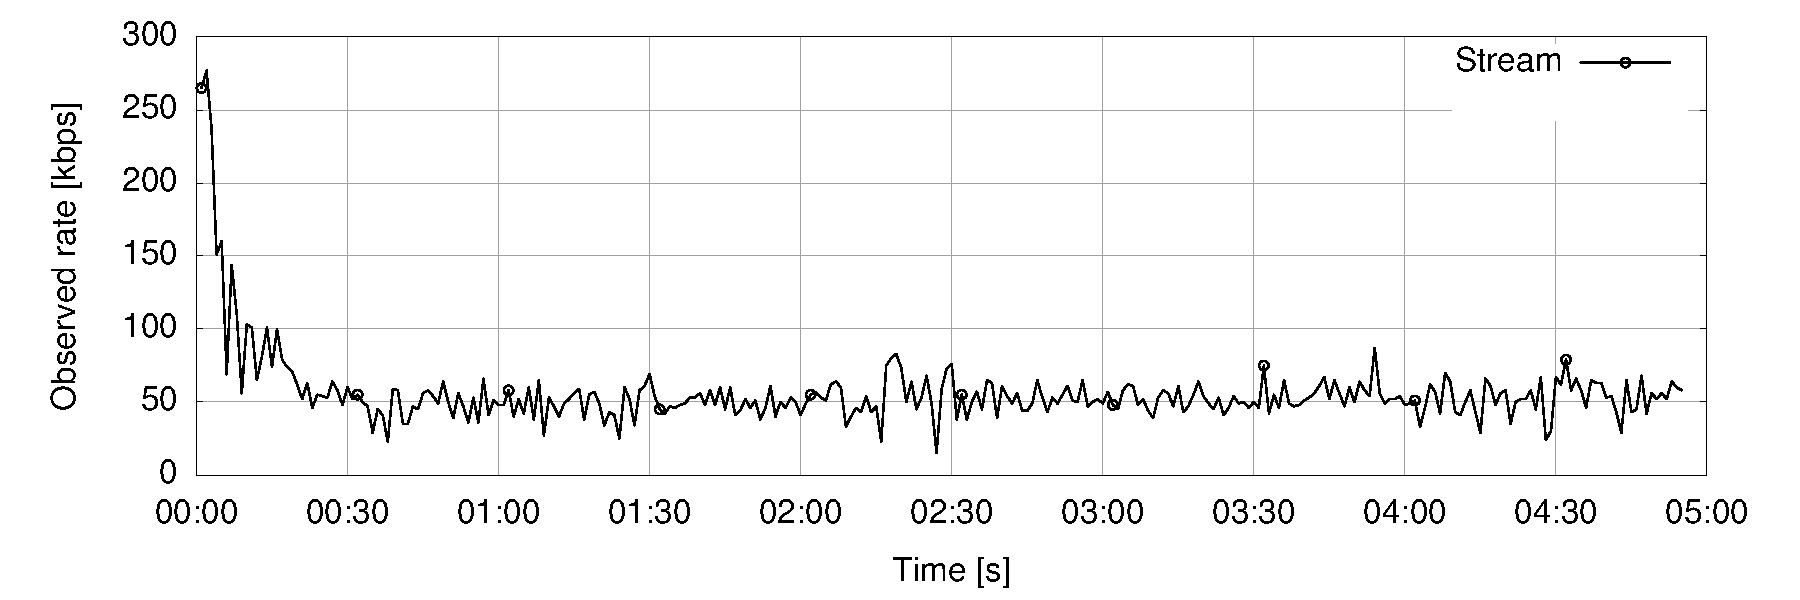
\includegraphics[width=1\textwidth]{./figures/plr10_rtt50ms_RV.pdf}
      \caption[Remote stream bandwidth for 10\% packet loss rate and 50ms delay]{Remote stream bandwidth for 10\% packet loss rate and 50ms delay.}
	\label{fig:bw_plr10_rtt50ms}
\end{figure}

Figure~\ref{fig:bw_plr10_rtt50ms} is an example that illustrates how the rate is lowered after the beginning of the call even the bandwidth is available. This is due to the formulas and mechanisms previously described.

Carrying delay and losses in the same path will not be handled by the congestion mechanisms in WebRTC giving a low rate output for the stream.

Another interesting factor around this test is the setup time that increases to up 4.6 seconds with 200ms delay and 3 seconds with 50ms, obviously this increase will also affect mobile developers when establishing calls in delayed environments.

\subsubsection{Bandwidth and queue variations}

We have also performed a different set of tests modifying the bandwidth and queue length. For this part of the test we have chosen to run 500 Kbit/s, 1, 5 and 10 Mbit/s with different queue sizes ranging from 100 ms, 500 ms, 1s and 10 s. In total we have run 12 different tests with ten iterations each.

The queue size is set in slots to {\it Dummynet} considering each slot as standard ethernet packet of 1500 Bytes, to calculate this number we use Equation~\ref{eq:QueueSize}.

\begin{equation}
	\frac{Bandwidth (Bits)}{8 \times 1500} \times Queue (seconds)
	\label{eq:QueueSize}
\end{equation}

We have seen a good response when having big queue sizes but larger deviation in bandwidth when reducing this queue size to 100 ms or 500 ms, this produced high delays over 20 ms for every call with different distribution curves. The delay that is given to the duration of the call is not stable and will affect the media flow, this increasing curve of delay distribution is given by the small queue size which produces bursty packets to arrive to the peer having different delay conditions.

When we tested the 5 Mbit/s case we got a high delay output even the bandwidth response adapted to the constraints, delay deviation is also high and will affect the time the packets arrive with large jittering.

We will study the result of the test performed at 1 Mbit/s limitation as the maximum standard bandwidth for WebRTC is approximately 2 Mbit/s, when having 1 Mbit/s limitation WebRTC will need to adapt the actual encoding rate and bandwidth control to that amount.

Figure~\ref{fig:1mb_mean_deviation_bw} represents the bandwidth and mean plotted for all the different tests performed in the 1 Mbit/s case. We can see that the response varies in small amount of bandwidth but with large deviation, when having 500ms and 1s queue size (\ref{fig:1mb_500ms_mean_deviation_bw}) we have much more deviation in means of packets being buffered in the relay. Otherwise, when the queue size reduces to 100ms (\ref{fig:1mb_100ms_mean_deviation_bw}) the deviation gets smaller but delay response is worst.

We can compare Figure~\ref{fig:1mb_total_delay_distribution} delay distribution results for the best case (\ref{fig:1mb_10s_total_delay_distribution}) and worst case (\ref{fig:1mb_01s_total_delay_distribution}). The delay response with large queue is better due to the rapid increase of packets that carry small delay, for the 100ms queue the curve is smoother having packets ranging in all values of delay between 0 and 130ms.

Delay experience with small queue sizes will be worst in the sense of the call flow, we might experience sudden delay situations that WebRTC won't be able to handle, when having larger queue sizes we son't notice the delay variations as much as with the previous example. Having a curvy increase in delay distribution figure will result in sudden delay variations in the call. The conclusion is that WebRTC is able to adapt to low capacity networks using its codec mechanism at the same time as it should improve the congestion control systems to adapt to different buffer sizes and queuing conditions. 

The congestion mechanisms in WebRTC will stabilize the rate until the amount of delay triggers the rate change to fit the new queue state requirements. Figure~\ref{fig:1cd81aa8-bw} and~\ref{fig:1cd81aa8-delay} show the bandwidth and delay for the same stream and how the rate adapts once the queues are full increasing the delay on the packets, rate is lowered and queues get empty giving producing low delay.

 \begin{figure}[h]
  \centering
    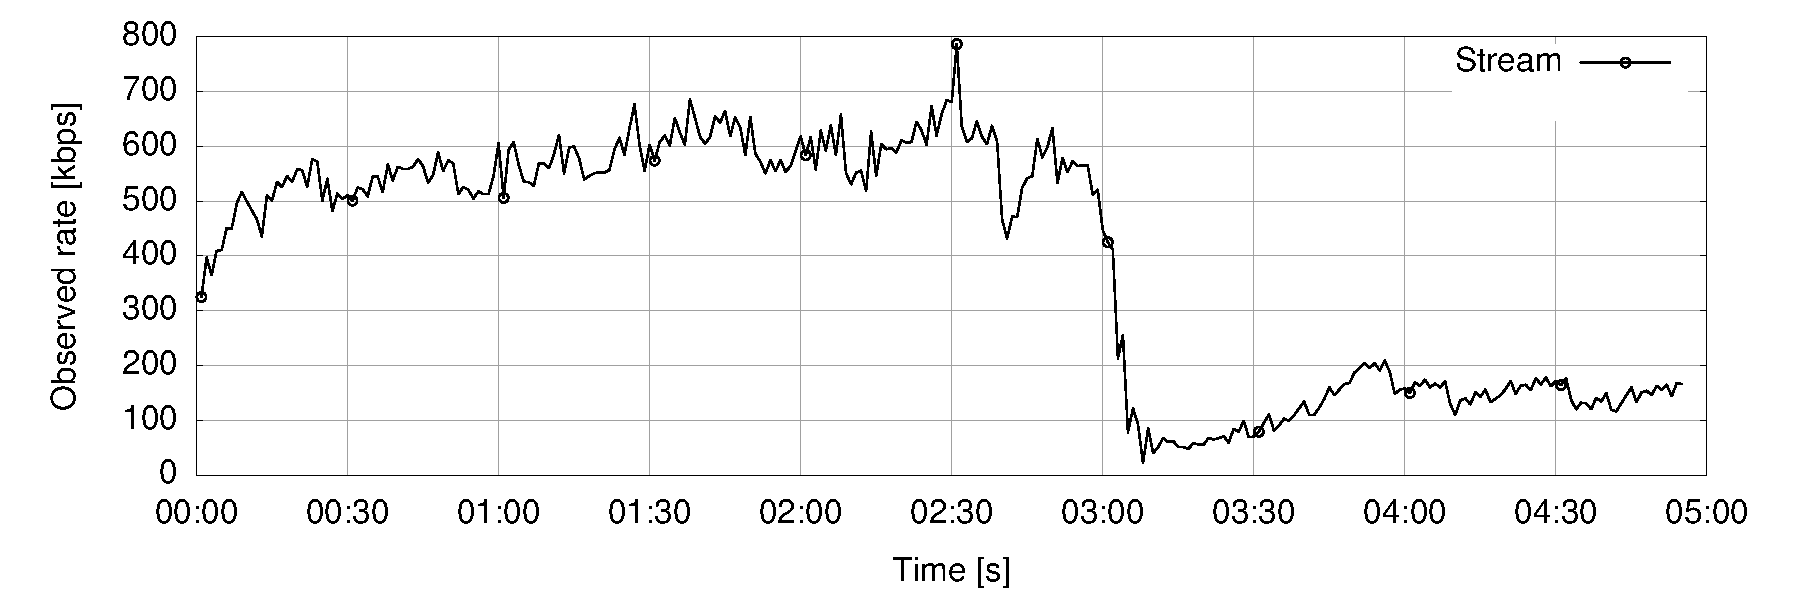
\includegraphics[width=1\textwidth]{./figures/1cd81aa8-bw.pdf}
      \caption[Remote stream bandwidth for 1 Mbit/s and 500ms queue size]{Remote stream bandwidth for 1 Mbit/s and 500ms queue size.}
	\label{fig:1cd81aa8-bw}
\end{figure}

 \begin{figure}[h]
  \centering
    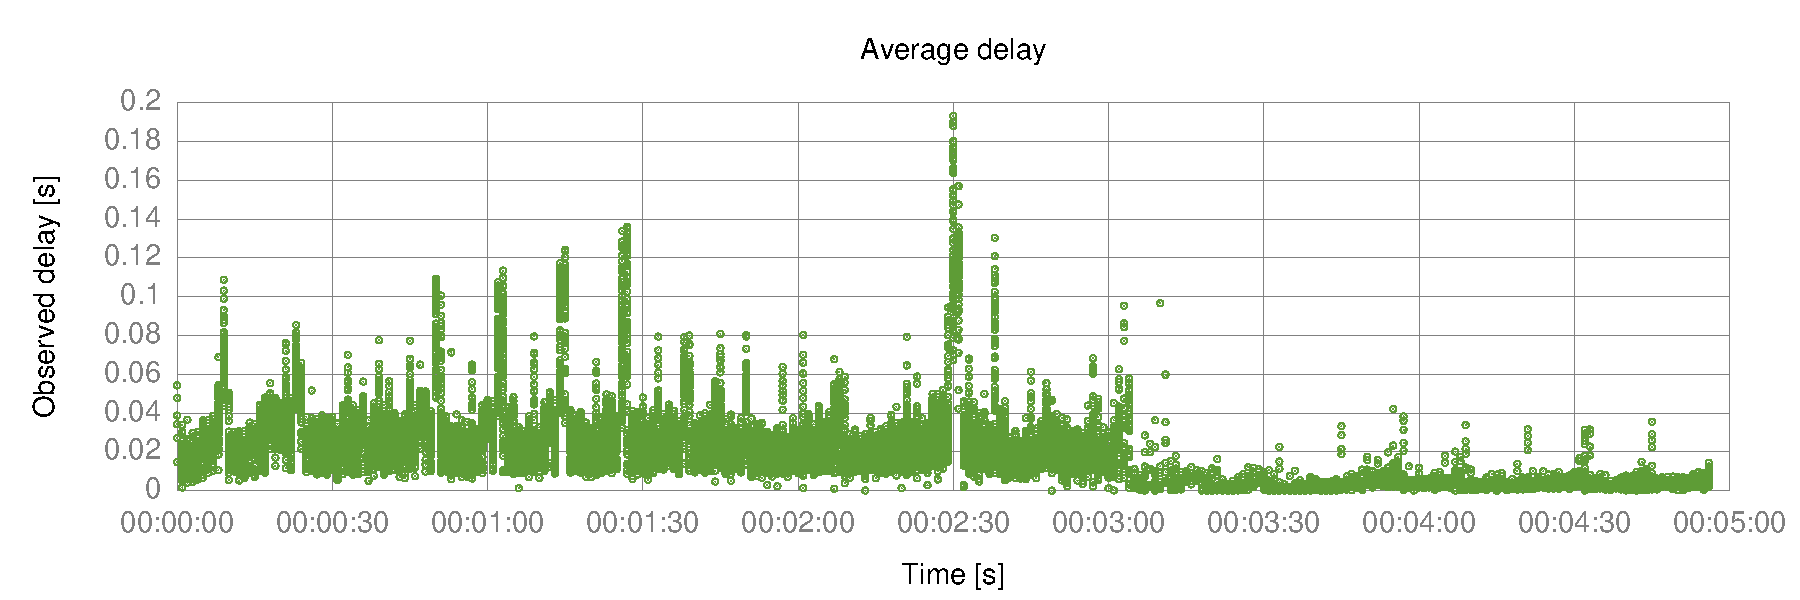
\includegraphics[width=1\textwidth]{./figures/1cd81aa8-delay.pdf}
      \caption[Stream delay for 1 Mbit/s and 500ms queue size]{Stream delay for 1 Mbit/s and 500ms queue size.}
	\label{fig:1cd81aa8-delay}
\end{figure}

Studying the way the sender takes decisions about rate constraints we can observe that the available bandwidth estimates calculated by the receiving side are only reliable when the size of the queues along the channel are large enough~\cite{alvestrandCongestion2012} . When having short queues along the path the maximum usage of the bandwidth cannot be estimated if there is no packet loss in the link, as in this case the packet loss is negligible, the connection is not able to use the maximum amount of bandwidth available in the link.

\begin{figure}[htp]
        \centering
        \begin{subfigure}[b]{1\textwidth}
                \centering
                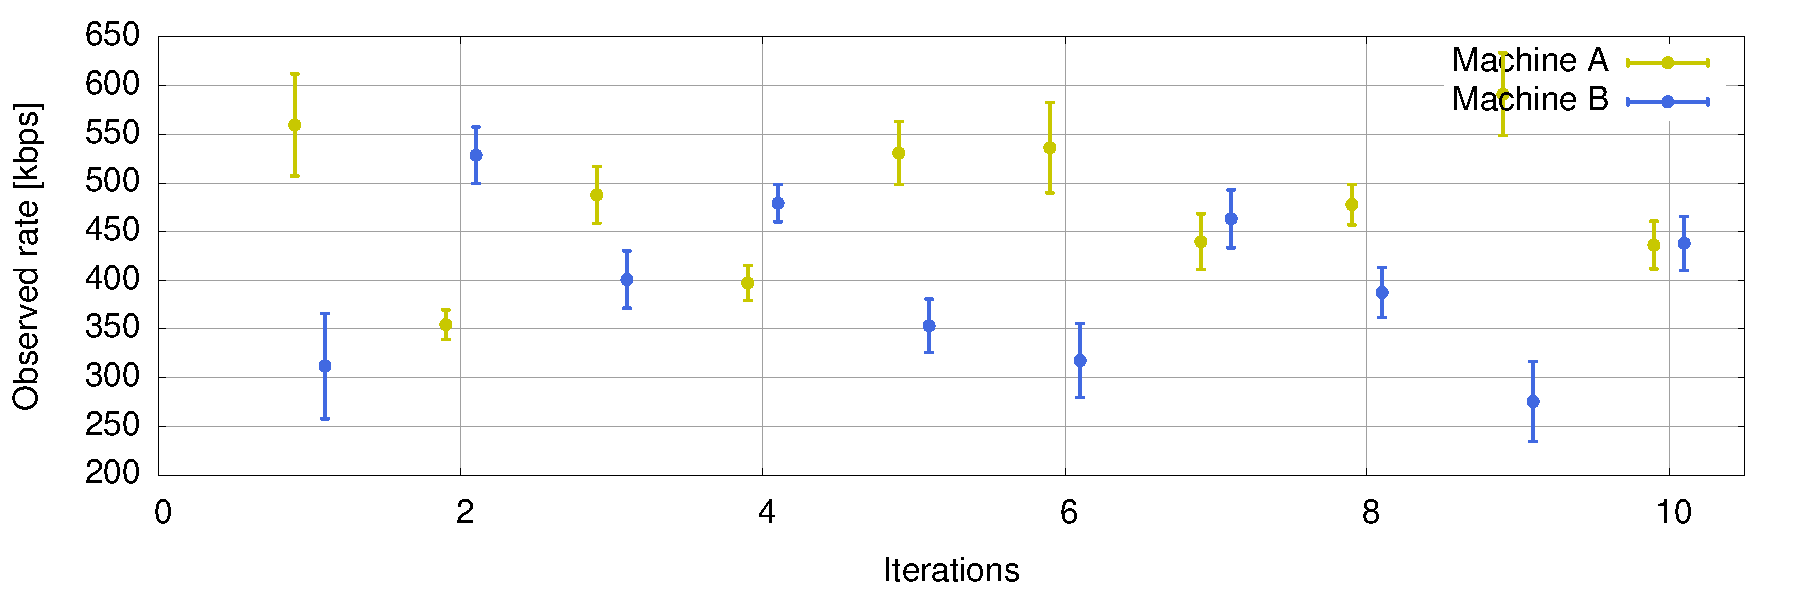
\includegraphics[width=\textwidth]{./figures/1mb_10s_mean_deviation_bw.pdf}
      \caption[1 Mbit/s and 10s queue size]{1 Mbit/s and 10s queue size.}
	\label{fig:1mb_10s_mean_deviation_bw}
        \end{subfigure}
        \qquad

        \begin{subfigure}[b]{1\textwidth}
                \centering
                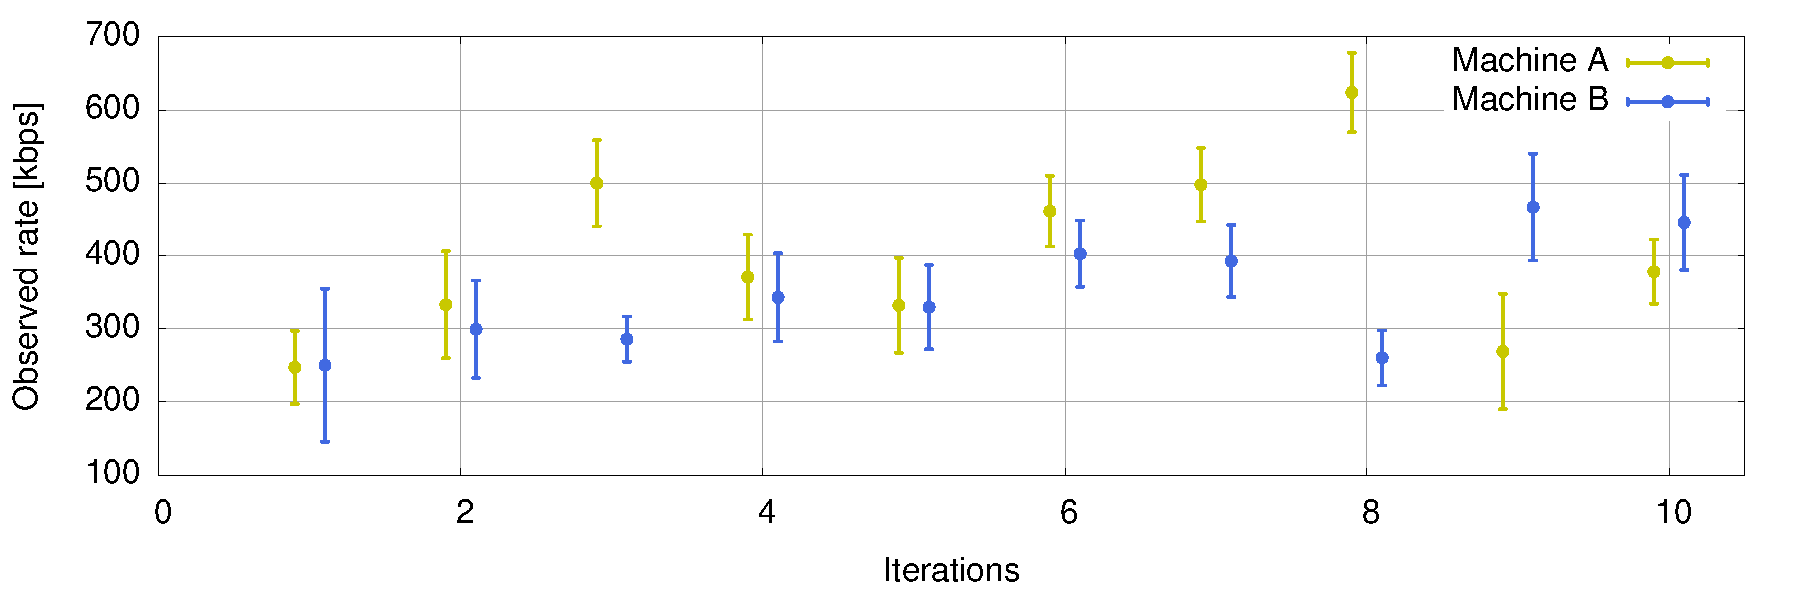
\includegraphics[width=\textwidth]{./figures/1mb_1s_mean_deviation_bw.pdf}
      \caption[1 Mbit/s and 1s queue size]{1 Mbit/s and 1s queue size.}
	\label{fig:1mb_1s_mean_deviation_bw}
        \end{subfigure}
        
        \begin{subfigure}[b]{1\textwidth}
                \centering
                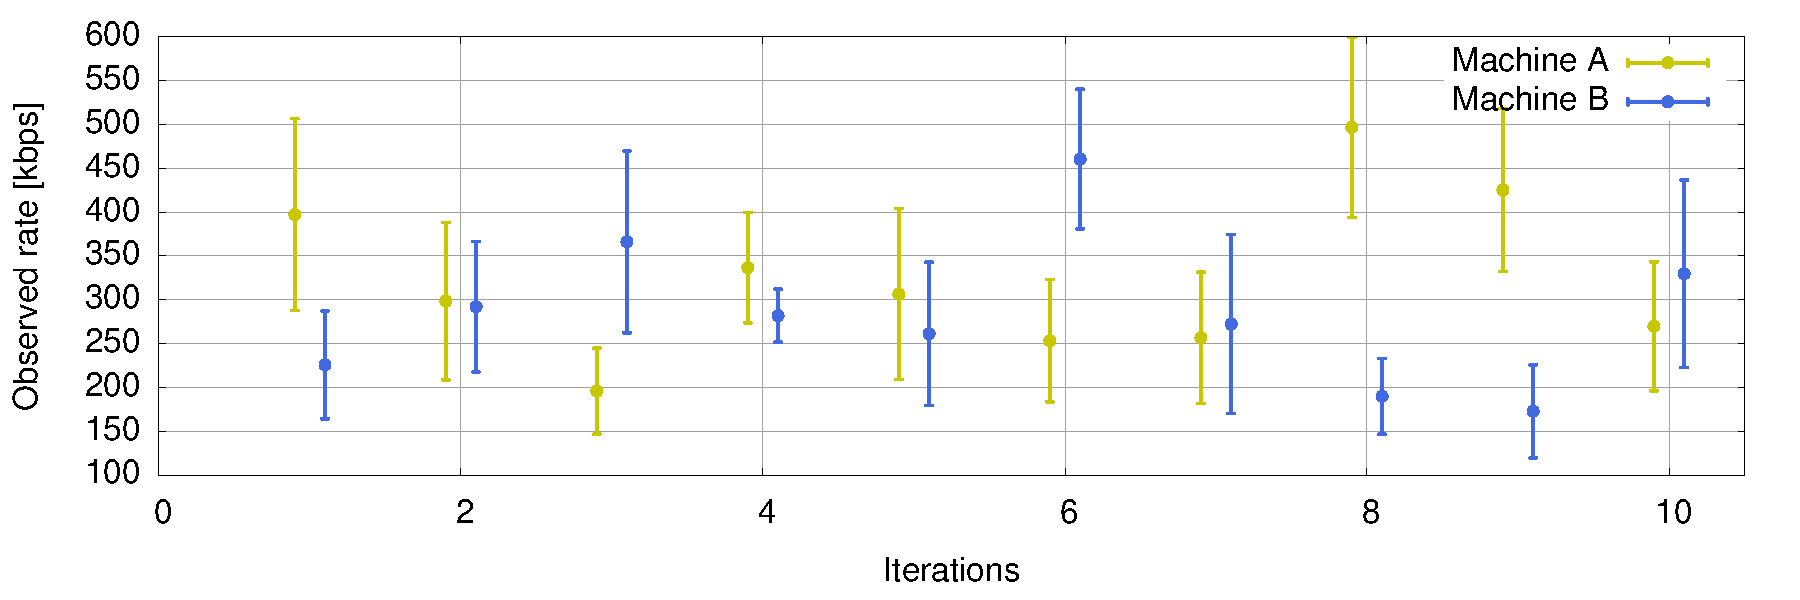
\includegraphics[width=\textwidth]{./figures/1mb_05s_mean_deviation_bw.pdf}
      \caption[1 Mbit/s and 500ms queue size]{1 Mbit/s and 500ms queue size.}
	\label{fig:1mb_500ms_mean_deviation_bw}
        \end{subfigure}
        \qquad

        \begin{subfigure}[b]{1\textwidth}
                \centering
                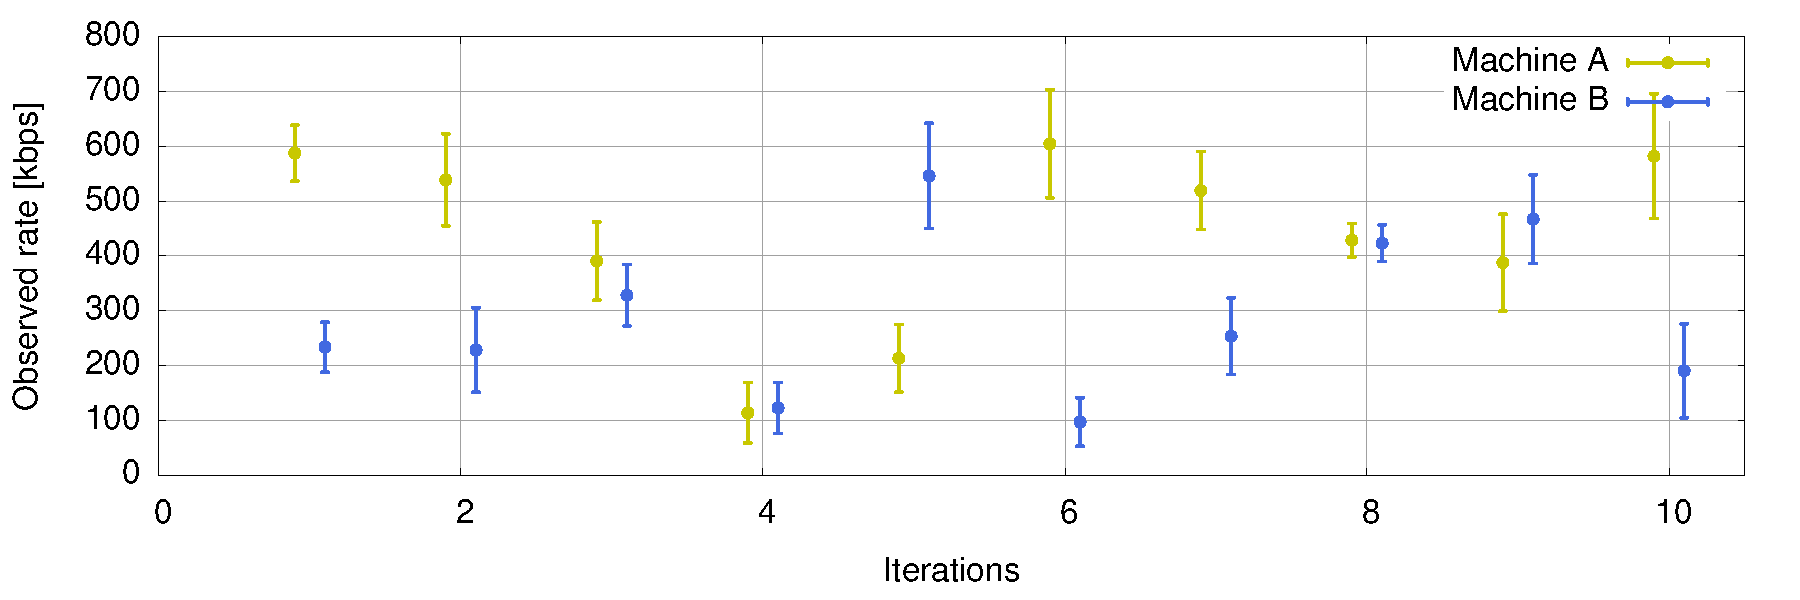
\includegraphics[width=\textwidth]{./figures/1mb_01s_mean_deviation_bw.pdf}
      \caption[1 Mbit/s and 100ms queue size]{1 Mbit/s and 100ms queue size.}
	\label{fig:1mb_01s_mean_deviation_bw}
        \end{subfigure}
        \caption{Bandwidth and mean for 1 Mbit/s with multiple queue sizes}
        \label{fig:1mb_mean_deviation_bw}
\end{figure}

\begin{figure}[htp]
        \centering
        \begin{subfigure}[h]{1\textwidth}
                \centering
                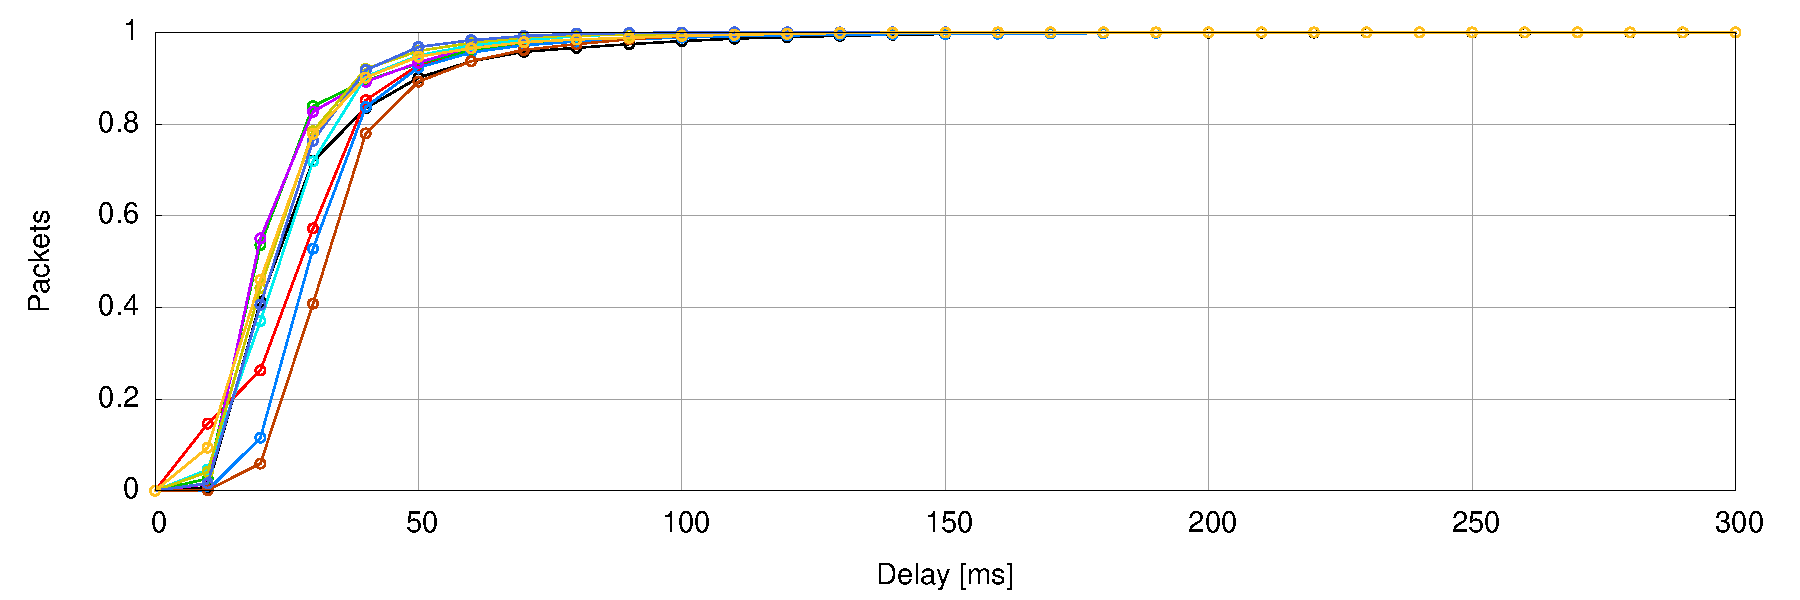
\includegraphics[width=\textwidth]{./figures/1mb_10s_total_delay_distribution.pdf}
      \caption[1 Mbit/s and 10s queue size]{1 Mbit/s and 10s queue size.}
	\label{fig:1mb_10s_total_delay_distribution}
        \end{subfigure}
        
        \begin{subfigure}[h]{1\textwidth}
                \centering
                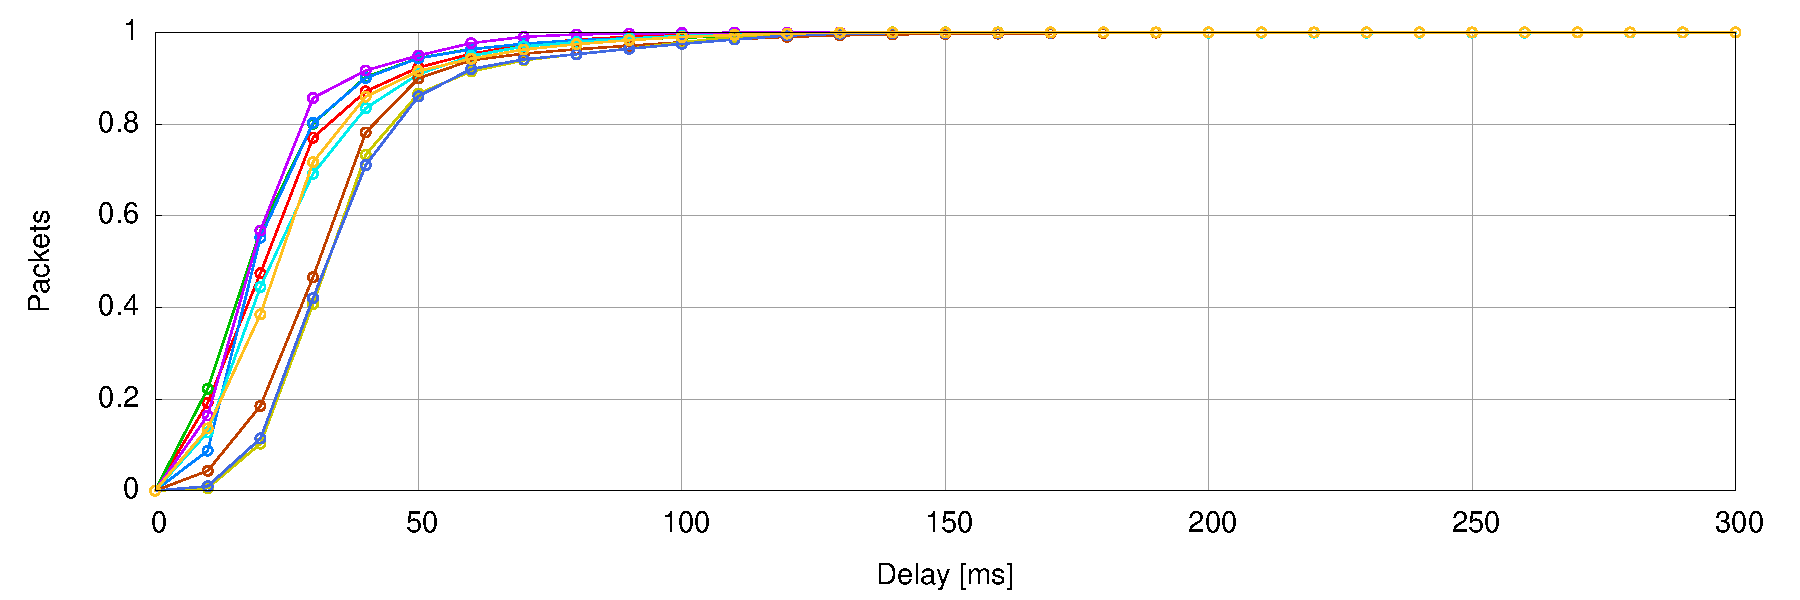
\includegraphics[width=\textwidth]{./figures/1mb_1s_total_delay_distribution.pdf}
      \caption[1 Mbit/s and 1s queue size]{1 Mbit/s and 1s queue size.}
	\label{fig:1mb_1s_total_delay_distribution}
        \end{subfigure}

        \begin{subfigure}[h]{1\textwidth}
                \centering
                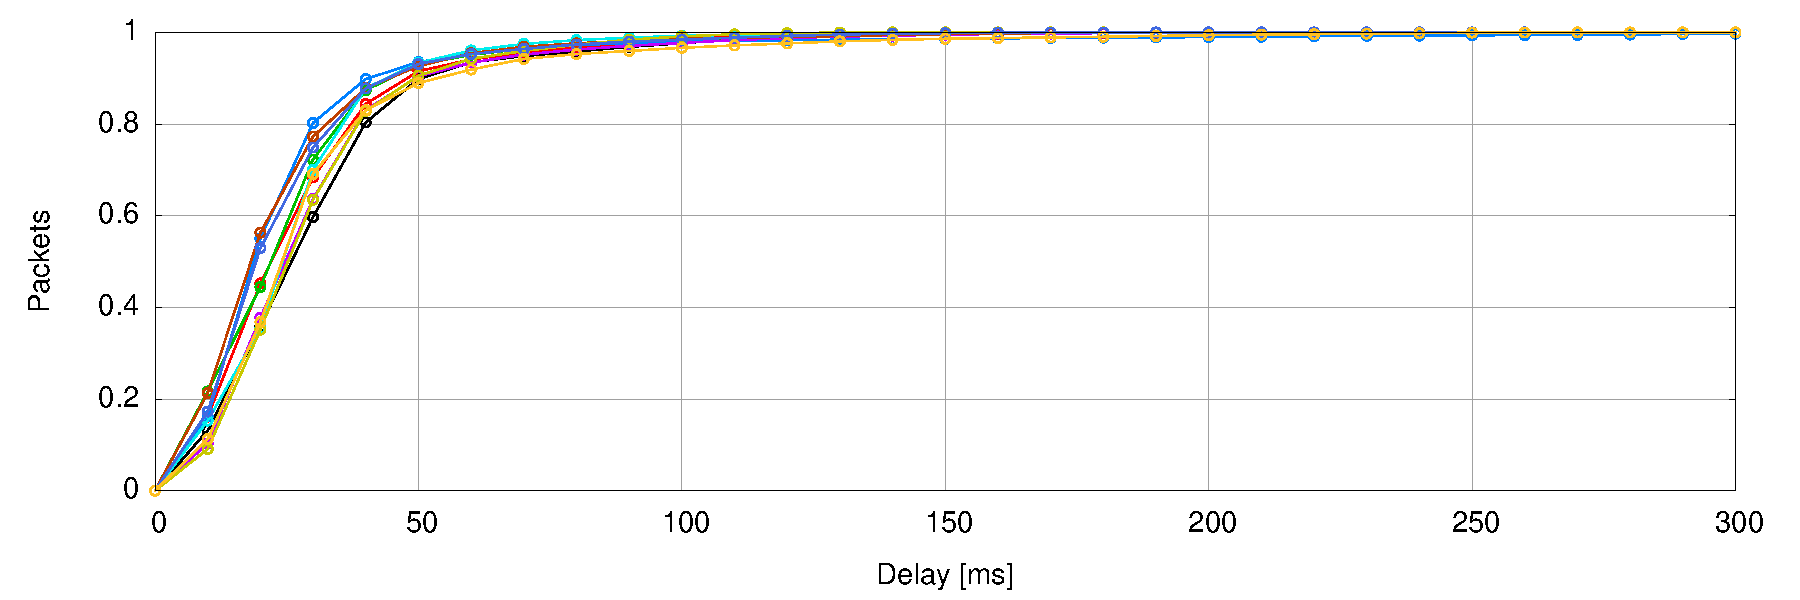
\includegraphics[width=\textwidth]{./figures/1mb_05s_total_delay_distribution.pdf}
      \caption[1 Mbit/s and 500ms queue size]{1 Mbit/s and 500ms queue size.}
	\label{fig:1mb_05s_total_delay_distribution}
        \end{subfigure}%
        
        \begin{subfigure}[h]{1\textwidth}
                \centering
                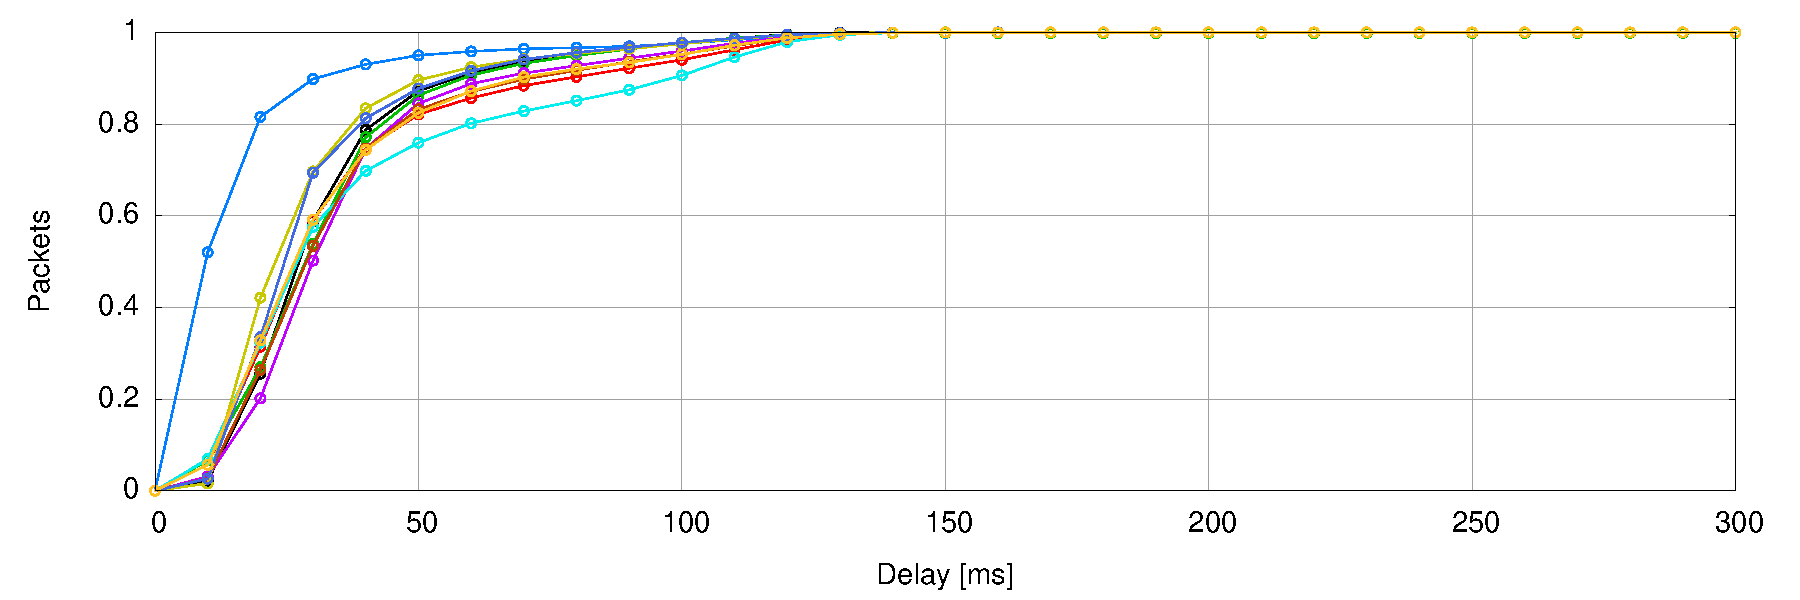
\includegraphics[width=\textwidth]{./figures/1mb_01s_total_delay_distribution.pdf}
      \caption[1 Mbit/s and 100ms queue size]{1 Mbit/s and 100ms queue size.}
	\label{fig:1mb_01s_total_delay_distribution}
        \end{subfigure}
        \caption{Delay distribution for 1 Mbit/s with multiple queue sizes}
        \label{fig:1mb_total_delay_distribution}
\end{figure}

\clearpage
\clearpage
\subsection{Loaded network}

Similar to the previous test, in this case we will be measuring the performance of WebRTC in a loaded network using a tool named {\it Iperf}. This tool will allow us to emulate traffic between our two peers loading the network according to our needs with UDP or TCP packets. The configuration we will use is the one shown in Figure~\ref{fig:iperfTest} with the clients running {\it Dummynet} instead of the relay. This scenario is chosen due its widely usage in real devices, having video calls meanwhile manipulating large amounts of online data is something that might happen when using WebRTC.

 \begin{figure}[h]
  \centering
    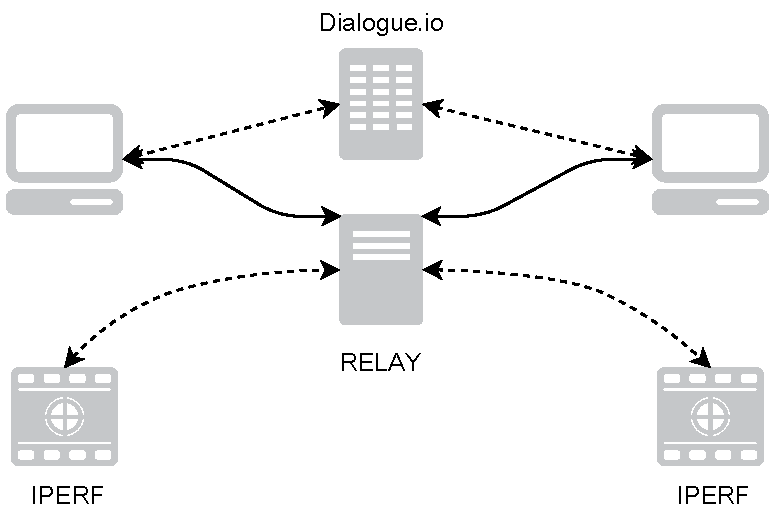
\includegraphics[width=0.8\textwidth]{./figures/IPERF.pdf}
      \caption[Topology for traffic flooded path using {\it Iperf}]{Topology for traffic flooded path using {\it Iperf}.}
	\label{fig:iperfTest}
\end{figure}

In this scenario we are interested in measuring also the behavior of real bandwidth setups for different environments, we will be testing the link with 100/10 Mbit/s and 20/4 Mbit/s limitations, the second one could be defined as the standard for HSPA networks. The data that will be sent to the other peer will be either 10 Mbit/s of TCP and UDP traffic or 2 Mbit/s.

First we will run the server as daemon on the recipient of the packets by executing:

\begin{verbatim}
# iperf -s -D
\end{verbatim}

The next step will rely on the usage of UDP or TCP, {\it Iperf} sends TCP packets by default, to do so we will run:

\begin{verbatim}
# iperf -c XXXX -t 300 {-u} -b 10m/2m 
\end{verbatim}

In the previous command, {\it -t} is the amount of time the test length, {\it -c} is the feature that configures the remote server to send the packets to, {\it -u} is going to be used to sent UDP datagrams instead of TCP and {\it -b} will define the amount of Mbit/s to be sent to the remote server. In this case every test is run three times.

Table~\ref{fig:tcp_iperf_no_dummynet} summarizes the results of the 10 Mbit/s TCP packet test without {\it Dummynet} constraints in the link.

\begin{table}[h]
\begin{center}
    \begin{tabular}{c D{,}{\pm}{-1} D{,}{\pm}{-1} D{,}{\pm}{-1} }
   	 \toprule
	\textit{}
	& \multicolumn{1}{c}{\textit{Machine A}}
	& \multicolumn{1}{c}{\textit{Machine B}}
	& \multicolumn{1}{c}{\textit{Overall}}\\
	\midrule
	\textbf{CPU (\%)} & 81.06 ,5.2 & 82.15 ,5.23 & 81.16 ,5.22\\
	\textbf{Memory (\%)} & 35.65 ,0.43 & 34.27 ,0.39 & 34.96 ,0.41\\
	\textbf{Bandwidth (Kbit/s)} & 990.11 ,202.62 & 1250.13 ,264.38 & 1120.12 ,233.506\\
	\textbf{Setup time (ms)} & 1533.66 ,11.3 & 1577.66 ,41.89 & 1555 ,32.59\\
	\textbf{RTT (ms)} & 25.61 ,16.02 & 24.76 ,14.11 & 25.19 ,15.07\\
	\textbf{Delay (ms)} & 81.61 ,11.42 & 83.99 ,11.42 & 81.61 ,11.42\\
	\bottomrule
    \end{tabular}
    \caption[IPERF 10 Mbit/s TCP test without link constraints]{IPERF 10 Mbit/s TCP test without link constraints.}
    \label{fig:tcp_iperf_no_dummynet}
\end{center}
\end{table}

The bandwidth rate in the call is affected by the traffic of TCP packets along the path, at the same time we are getting higher delays. Call behavior in this environment changes in every iteration being unpredictable, Figure~\ref{fig:iperfTestStd} represents the bandwidth mean and deviation of every iteration, we can easily observe that in the worst case we are getting three times less rate than the optimum case, ranging from 1.5 Mbit/s to under 400 Kbit/s in the worst iteration.

 \begin{figure}[h]
  \centering
    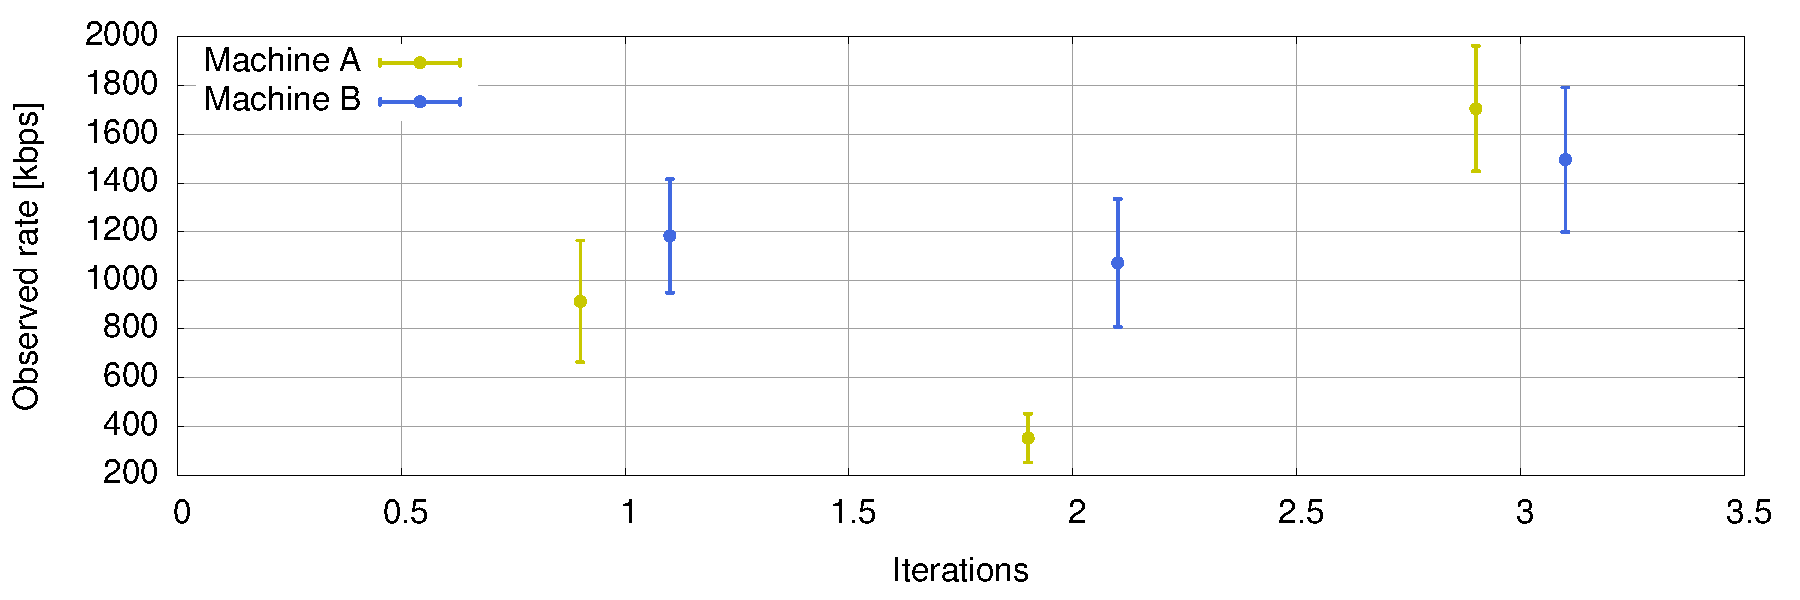
\includegraphics[width=1\textwidth]{./figures/iperf_std_mean_deviation_bw.pdf}
      \caption[Bandwidth mean and deviation for 10 Mbit/s TCP {\it Iperf} test without link constraints]{Bandwidth mean and deviation for 10 Mbit/s TCP {\it Iperf} test without link constraints.}
	\label{fig:iperfTestStd}
\end{figure}

We can observe some interesting behavior in all three iterations when looking at Figure~\ref{fig:iperfTestStdDelay} total delay distribution, the response varies from all three tests being all of them bad, a lot of sudden delay changes will appear during the call making real time communication difficult. The delay deviation is small but the tolerance for TCP flooded networks is low int WebRTC.

 \begin{figure}[h]
  \centering
    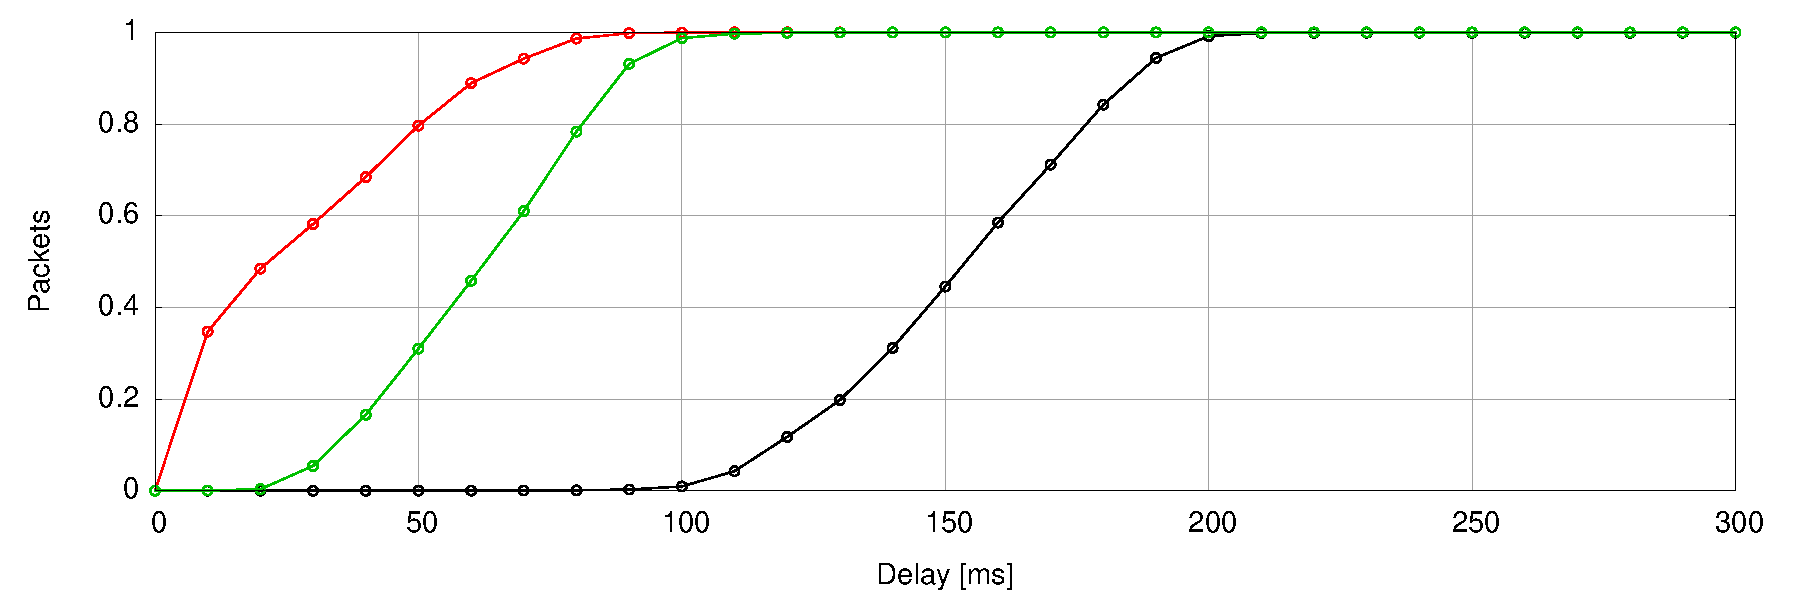
\includegraphics[width=1\textwidth]{./figures/iperf_std_total_delay_distribution.pdf}
      \caption[Total delay distribution for 10 Mbit/s TCP {\it Iperf} test without link constraints]{Total delay distribution for 10 Mbit/s TCP {\it Iperf} test without link constraints.}
	\label{fig:iperfTestStdDelay}
\end{figure}

Now we will test the behavior when sending those 10 Mbit/s with UDP and TCP in a constrained link of 100/10 (downlink/uplink), in this test {\it Dummynet} scripts have been executed on the client side instead of in the Relay. Table~\ref{fig:tcp_iperf_100in_10out} shows the different bandwidth responses between TCP and UDP traffic, in both cases the link constraint have been the same but the result varies. We will se an increase of rate with TCP flooded packets but also an increase of delay, this delay might be produced due the need of processing more packets with TCP than the simple mechanism of UDP.

\begin{table}[h]
\begin{center}
    \begin{tabular}{c D{,}{\pm}{-1} D{,}{\pm}{-1} D{,}{\pm}{-1} }
   	 \toprule
	\textit{}
	& \multicolumn{1}{c}{\textit{Machine A}}
	& \multicolumn{1}{c}{\textit{Machine B}}
	& \multicolumn{1}{c}{\textit{Overall}}\\
	\midrule
	\textbf{Bandwidth UDP (Kbit/s)} & 159.41 ,28.69 & 149.04 ,25.76 & 159.23 ,27.23 \\
	\textbf{Delay UDP (ms)} & 98.07 ,3.14 & 98.85 ,2.75 & 96.85 ,2.94 \\
	\hline
	\hline
	\textbf{Bandwidth TCP (Kbit/s)} & 208.97 ,20.64 & 194.41 ,18.9 & 201.69 ,19.77\\
	\textbf{Delay TCP (ms)} & 146.9 ,4.38 & 147.92 ,4 & 147.41 ,4.23 \\
	\bottomrule
    \end{tabular}
    \caption[IPERF 10 Mbit/s TCP and UDP test with constrained 100/10 Mbit/s link]{IPERF 10 Mbit/s TCP and UDP test with constrained 100/10 Mbit/s link.}
    \label{fig:tcp_iperf_100in_10out}
\end{center}
\end{table}

Delay distribution response in a constrained environment (Figure~\ref{fig:10m_udp_total_delay_distribution} and \ref{fig:10m_tcp_total_delay_distribution}) is smoother compared to Figure~\ref{fig:iperfTestStdDelay}, the absolute amount of delay is larger but the distribution curve is better for WebRTC needs as it does not have any sudden increase of delay. Delay response when having constraints will output a better delay distribution but with higher RTT in the link.

\begin{figure}
        \centering
        \begin{subfigure}[b]{0.5\textwidth}
                \centering
                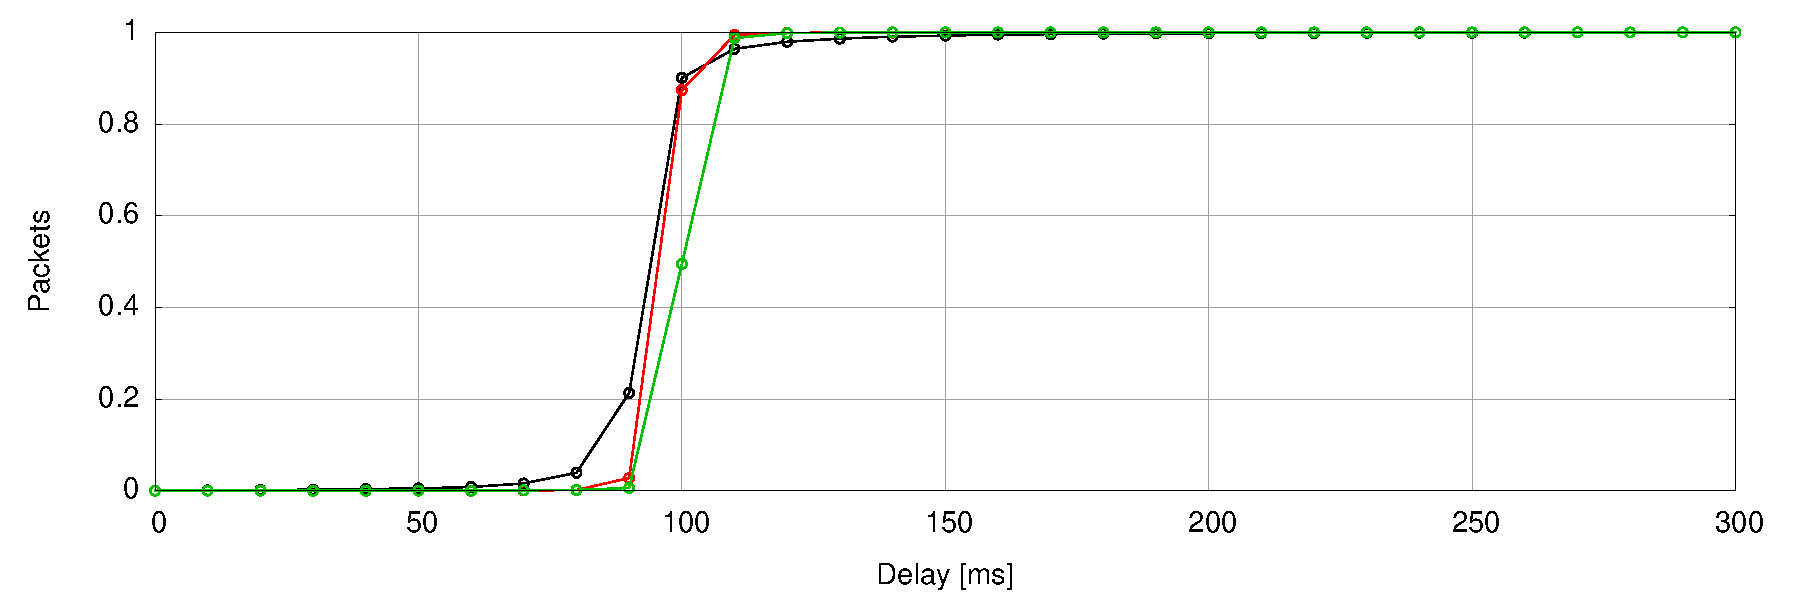
\includegraphics[width=\textwidth]{./figures/10m_udp_total_delay_distribution.pdf}
                \caption{Delay distribution response for UDP test}
                \label{fig:10m_udp_total_delay_distribution}
        \end{subfigure}%
        ~ %add desired spacing between images, e. g. ~, \quad, \qquad etc.
          %(or a blank line to force the subfigure onto a new line)
        \begin{subfigure}[b]{0.5\textwidth}
                \centering
                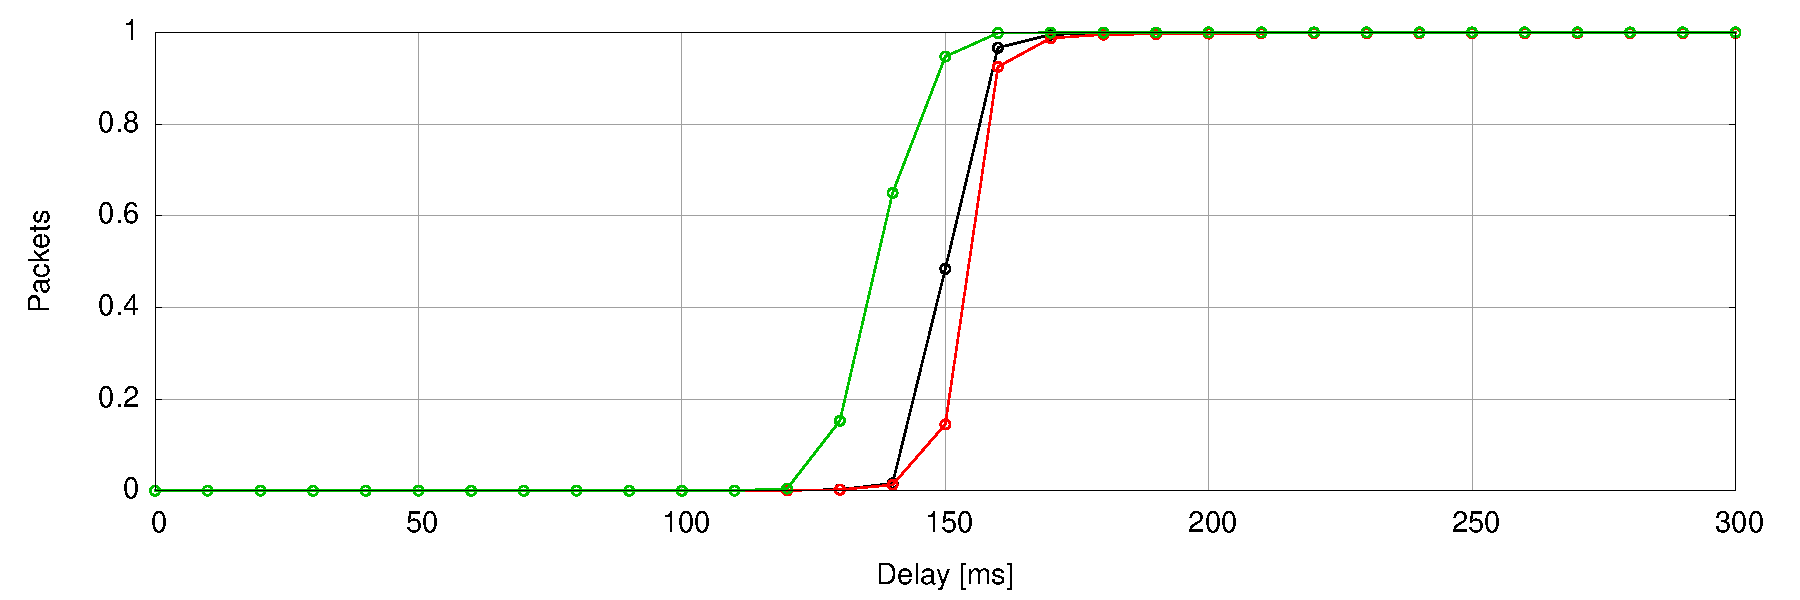
\includegraphics[width=\textwidth]{./figures/10m_tcp_total_delay_distribution.pdf}
                \caption{Delay distribution response for TCP test}
                \label{fig:10m_tcp_total_delay_distribution}
        \end{subfigure}
        \caption[10 Mbit/s UDP/TCP {\it Iperf} test with 100/10 link condition]{10 Mbit/s UDP/TCP {\it Iperf} test with 100/10 link condition.}
        \label{fig:10m_tcp_udp_distribution}
\end{figure}

When testing the 2 Mbit/s TCP and UDP flows with 20/4 Mbit/s constraints results are surprisingly close to the version without constraints, we are testing this configuration due to its similitudes to HSDPA networks that carry a similar averaged bandwidth. Unstable bandwidth is also noticed in this test but values for the rate are much higher and delay distribution graphs are similar to Figure~\ref{fig:10m_tcp_udp_distribution}. We are using 2 Mbit/s flows to imitate the encoding rate for an online streaming 1280x720 HD video.\footnote{http://www.adobe.com/devnet/adobe-media-server/articles/dynstream_live/popup.html}

Table~\ref{fig:tcp_iperf_20in_4out} describes the output we had in terms of rate and delay for the 2 Mbit/s test in a HSDPA type network. Rate adaptation is good even having an small uplink capacity of 4 Mbit/s, the way the rate is adapted to this link confirms that in this kind of not delayed or lossy low latency networks WebRTC could perform properly with simultaneous ongoing traffic. 

\begin{table}[h]
\begin{center}
    \begin{tabular}{c D{,}{\pm}{-1} D{,}{\pm}{-1} D{,}{\pm}{-1} }
   	 \toprule
	\textit{}
	& \multicolumn{1}{c}{\textit{Machine A}}
	& \multicolumn{1}{c}{\textit{Machine B}}
	& \multicolumn{1}{c}{\textit{Overall}}\\
	\midrule
	\textbf{Bandwidth UDP (Kbit/s)} & 683.81 ,259.38 & 749.66 ,249.69 & 716.74 ,254.53 \\
	\textbf{Delay UDP (ms)} & 56.34 ,2.83 & 54.31 ,2.64 & 55.32 ,2.74 \\
	\hline
	\hline
	\textbf{Bandwidth TCP (Kbit/s)} & 760.94 ,238.44 & 1174.95 ,235.12 & 967.94 ,236.78\\
	\textbf{Delay TCP (ms)} & 85.18 ,2.3 & 80.04 ,2.26 & 82.61 ,2.28 \\
	\bottomrule
    \end{tabular}
    \caption[IPERF 2 Mbit/s TCP and UDP test with constrained 20/4 Mbit/s link]{IPERF 2 Mbit/s TCP and UDP test with constrained 20/4 Mbit/s link.}
    \label{fig:tcp_iperf_20in_4out}
\end{center}
\end{table}

From the delay distribution point of view (Figure~\ref{fig:2m_tcp_udp_distribution}), the output is similar in both tests being TCP slightly better (\ref{fig:2m_tcp_total_delay_distribution}) with less absolute delay and with an acceptable variation.

\begin{figure}
        \centering
        \begin{subfigure}[b]{0.5\textwidth}
                \centering
                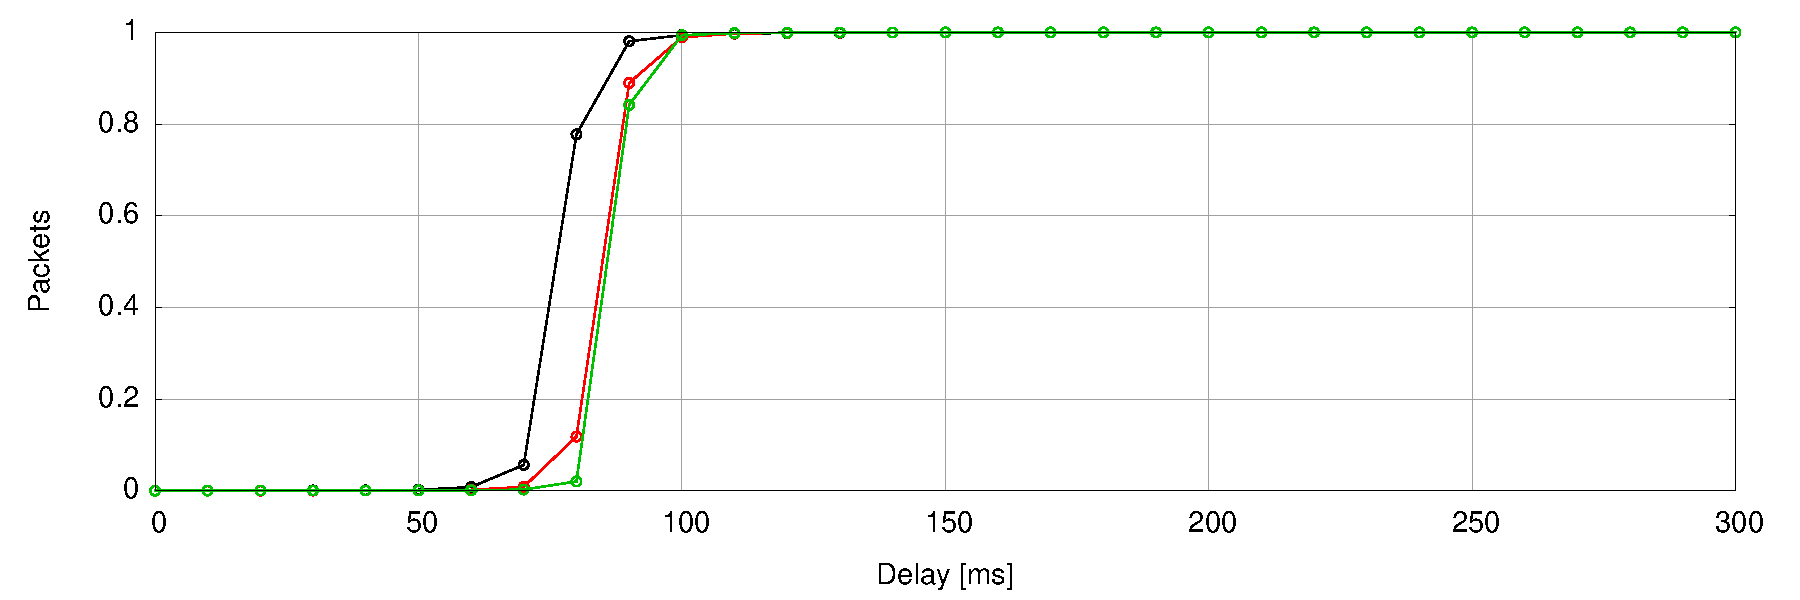
\includegraphics[width=\textwidth]{./figures/2m_udp_total_delay_distribution.pdf}
                \caption{Delay distribution response for UDP test}
                \label{fig:2m_udp_total_delay_distribution}
        \end{subfigure}%
        ~ %add desired spacing between images, e. g. ~, \quad, \qquad etc.
          %(or a blank line to force the subfigure onto a new line)
        \begin{subfigure}[b]{0.5\textwidth}
                \centering
                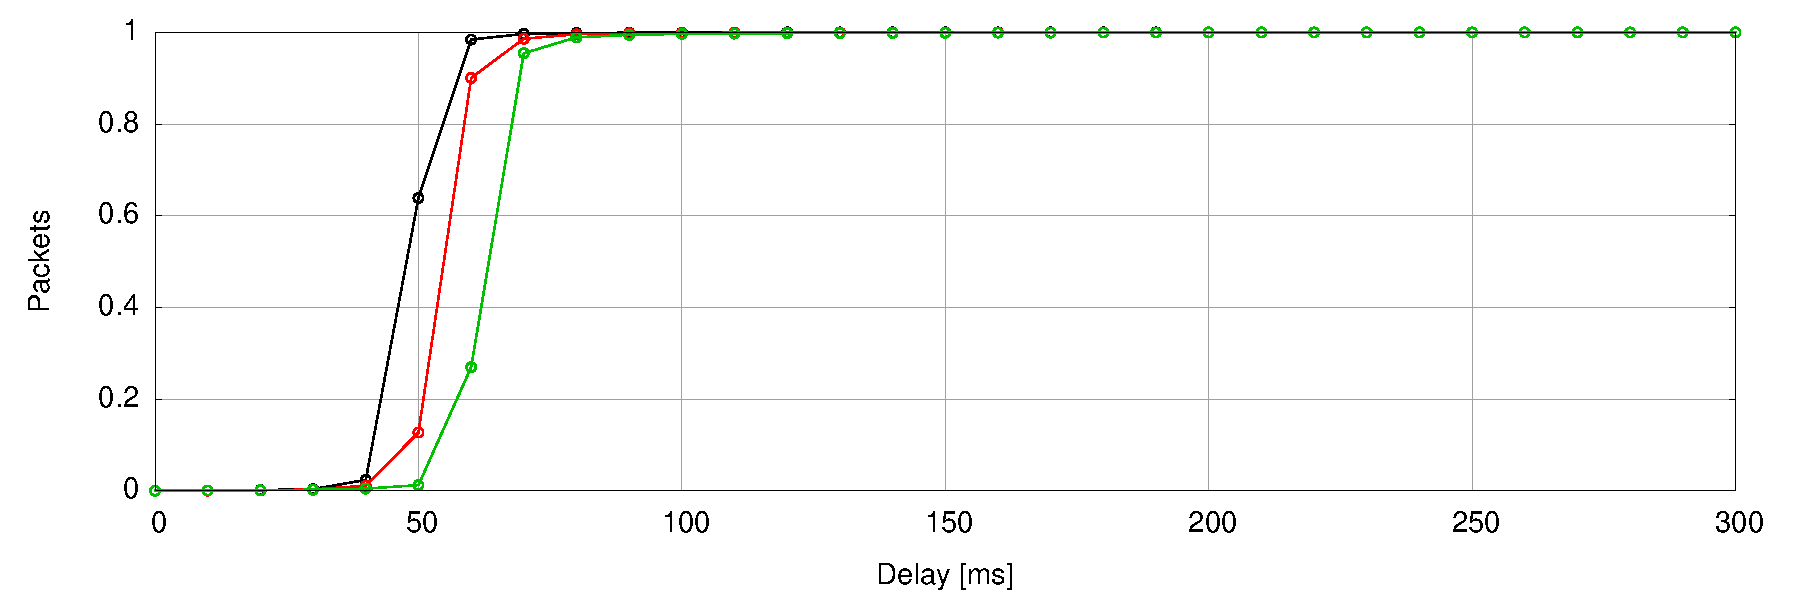
\includegraphics[width=\textwidth]{./figures/2m_tcp_total_delay_distribution.pdf}
                \caption{Delay distribution response for TCP test}
                \label{fig:2m_tcp_total_delay_distribution}
        \end{subfigure}
        \caption[2 Mbit/s UDP and TCP {\it Iperf} test with 20/4 link condition]{2 Mbit/s UDP and TCP {\it Iperf} test with 20/4 link condition.}
        \label{fig:2m_tcp_udp_distribution}
\end{figure}

In general, the response of WebRTC congestion mechanisms with ongoing link traffic should be better as this environment will be common for all users. The bandwidth mechanism produces an acceptable call rate but should produce delays smaller than one second which are acceptable from the usability perspective, the delay distribution for the standard case with an ongoing traffic of 10 Mbit/s is not as good as expected but it might be due to the high capacity on the path and the way {\it Iperf} simulates the traffic.

\subsection{Parallel calls}

In this part of the test we will be checking how WebRTC handles multiple parallel calls with different peers, this is not to me mixed with mesh style of topology as it will be running using different tabs or processes through the same TURN path. Figure~\ref{fig:parallelCalls} represents the topology used for the test.

 \begin{figure}[h]
  \centering
    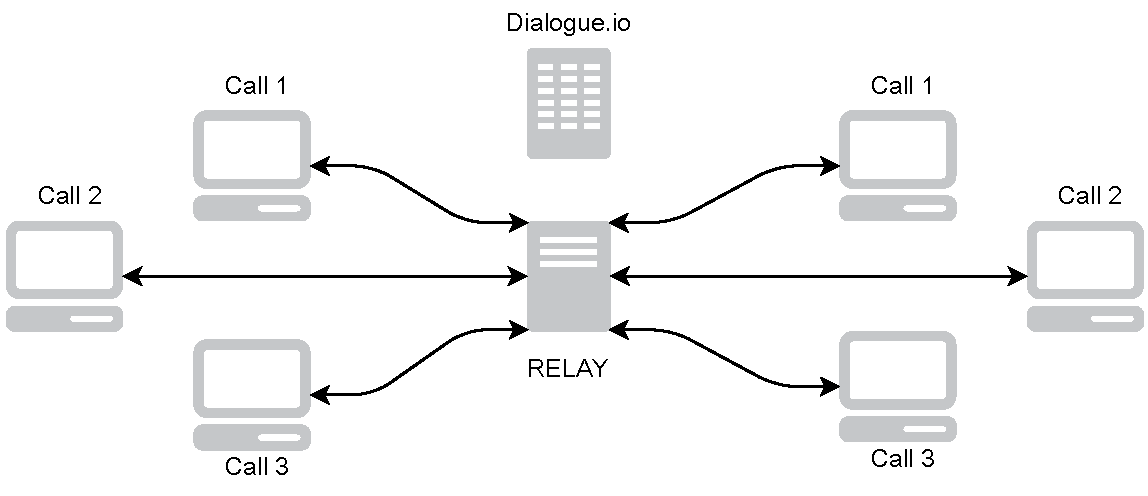
\includegraphics[width=1\textwidth]{./figures/ParallelCalls.pdf}
      \caption[Topology for three different parallel calls using the same link]{Topology for three different parallel calls using the same link.}
	\label{fig:parallelCalls}
\end{figure}

We will run a combined batch of tests using 2 and 3 simultaneous calls without {\it Dummynet} or with 20 Mbit/s and 10 Mbit/s bandwidth limitation for the link. The case without any constraint will run with the standard 100 Mbit/s of the ethernet link capacity. For the test we have focused in running the calls in the same machine but in different processes.

This kind of environment will be given in local networks or it could be compared with mesh topologies handling multiple peer connections, from the resources perspective it will be interesting to observe the CPU and memory consumption as every PeerConnection will be working in a different process, the machine used carries 1 CPU and 2 Gb of RAM.

\begin{table}[h]
\begin{center}
    \begin{tabular}{c D{,}{\pm}{-1} D{,}{\pm}{-1} D{,}{\pm}{-1} }
   	 \toprule
	\textit{}
	& \multicolumn{1}{c}{\textit{CPU (\%)}}
	& \multicolumn{1}{c}{\textit{Memory (\%)}}\\
	\midrule
	\textbf{Three calls} & 99.25 ,2.41 & 44.99 ,0.5 \\
	\textbf{Two calls 20 Mbit/s} & 95.67 ,3.51 & 46.16 ,0.37 \\
	\textbf{Two calls 10 Mbit/s} & 86.83 ,5.03 & 44.91 ,0.32 \\
	\textbf{Two calls} & 81.6 ,6.48 & 42.61 ,0.35 \\
	\bottomrule
    \end{tabular}
    \caption[Memory and CPU consumption rates for parallel calls in different link conditions]{Memory and CPU consumption rates for parallel calls in different link conditions.}
    \label{fig:cpu_mem_parallel}
\end{center}
\end{table}

Table~\ref{fig:cpu_mem_parallel} describes the resource comparison between two and three simultaneous calls. CPU usage is critical when handling three peer connections or when the network condition forces the congestion mechanism to continuously adapt the bandwidth and encoding. In this test, each call is placed in a different process which should improve the results as the OS will handle them better than in a single thread. When the CPU load gets to its maximum the performance of WebRTC for encoding/decoding and transmission is deprecated, in this kind of topologies having high CPU performance increases the call quality.

\begin{table}[h]
\begin{center}
    \begin{tabular}{c D{,}{\pm}{-1} D{,}{\pm}{-1} D{,}{\pm}{-1} }
   	 \toprule
	\textit{}
	& \multicolumn{1}{c}{\textit{Machine A}}
	& \multicolumn{1}{c}{\textit{Machine B}}
	& \multicolumn{1}{c}{\textit{Overall}}\\
	\midrule
	\textbf{Three calls} & 768.04 ,180.93 & 850.1 ,223.84 & 809.07 ,202.38 \\
	\textbf{Two calls 20 Mbit/s} & 432.56 ,141.32 & 531.13 ,169.82 & 481.85 ,155.56 \\
	\textbf{Two calls 10 Mbit/s} & 178.83 ,60.05 & 141.83 ,42.02 & 160.24 ,51.04 \\
	\textbf{Two calls} & 392.08 ,181.9 & 545.94 ,259.27 & 469.01 ,221.09 \\
	\bottomrule
    \end{tabular}
    \caption[Bandwidth rates for parallel calls in different link conditions]{Bandwidth rates for parallel calls in different link conditions.}
    \label{fig:bw_parallel}
\end{center}
\end{table}


%Summary of results
%\include{./chapters/summary}

%Discussion
%\include{./chapters/discussion}

%Real use case (dialogue.io)
%\include{./chapters/dialogue}

%%conclusion chapter
\section{Conclusion}

%% 
%% Leave first page empty
\thispagestyle{empty}

During the development of this thesis we have analyzed and evaluated WebRTC protocol for real-time web applications in different environments. We also compared this protocol with already existing real-time communications alternatives and described the usage of the actual implementation of WebRTC. Furthermore, we also decided a set of key indicators that are important when measuring the performance of a RTC protocol. Those indicators are used when evaluating the congestion control mechanisms of WebRTC. We also described the possible real-time topologies used to test the performance of WebRTC, some of them are still not possible to implement due to API constraints. To evaluate the protocol we also built an specific setup for this thesis, the environment is used during the development of all the thesis. Finally, we executed the tests after describing the proposed congestion control mechanisms and the ones already implemented in WebRTC.

After the tests, we can conclude that WebRTC is a solid protocol for real-time web applications that performs correctly in constrained environments with low latencies, up to 200ms, but cannot hold greater values. This condition may affect mobile applications relying on WebRTC. The congestion control mechanism implemented in WebRTC, Receiver-side Real-time Congestion Control (RRTCC), copes correctly with packet losses protecting the packets with different mechanisms such as Forward Error Correction (FEC). To improve the performance of WebRTC, different congestion control mechanisms that react to other indicators could be implemented in the internals of the browsers.

Furthermore, some future investigations could be done in order to determine the usability limits of WebRTC. Future works include a deeper experience in mobile environments with the two possible implementations: native mobile application and mobile web application. Both are crucial for the expansion of WebRTC into mobile platforms. Besides this, the analysis of WebRTC session on mobile moving nodes is also important to check the response of the call quality.

WebRTC APIs also need enhancements in order to test all possible environments. One of the most interesting areas to investigate, is the development of a transcoding MCU in WebRTC. During this thesis we have used a packet relying MCU environment for the tests, the transcoding MCU multiplexes and mixes the media streams into a unique channel to improve performance over the path. This type of environment is commonly used for multiparty calls. A better understanding of the Stats API implemented in WebRTC is also needed to better adequate the constraints of the media acquisition and the PeerConnection API. Those metrics are provided by the browser internals and can provide valuable feedback for the application developer that can be used to improve the quality of the session.

Lastly, a follow-up of the cross-compatibility of the browser congestion control mechanisms should be studied in order to provide full interoperability between vendors and devices. At the development of this thesis, this compatibility is not achieved due to the lack of congestion control mechanisms in some browser providers.



\addcontentsline{toc}{section}{References}
\bibliographystyle{unsrt}
\bibliography{./chapters/allpapers} 

%%Appendix
\appendix
\section{Setting up fake devices in Google Chrome}
\label{sec:fakeVideo}

%% 
%% Leave first page empty
\thispagestyle{empty}

To address the issue of the video transferred from our automated devices we have built a fake input device on the virtual machines that is fed with a RAW YUV file. This device is configured using a hacked version of the {\it V4L2Loopback} code which is originated from the {\it V4L} driver in Linux. The modified version of the {\it V4L2Loopback} builds two extra devices in the Linux interface mapping. This is done as Chrome is unable to read from the same reading/writing device for security reasons. The first device is used to fed the video and the other one to read it~\cite{chromiumIssue142568} in an input/output configuration. 

The following additions have been done in the {\it V4L2Loopback} code:

\begin{itemize}
	\item Need to write a non-null value into the the bus information of the device, this is required as Chrome input needs to be named as a real device. When using Firefox this is not required but works as well.
\end{itemize}

\lstset{language=C}
\begin{lstlisting}
strlcpy(cap->bus_info, "virtual", sizeof(cap->bus_info));
\end{lstlisting}
\begin{itemize}
	\item Our driver will pair devices when they are generated, this will create one read device and one capture device. Everything written into {\it /dev/video0} will be read from {\it /dev/video1}. 
\end{itemize}

\lstset{language=C}
\begin{lstlisting}
cap->capabilities |= V4L2_CAP_VIDEO_OUTPUT | V4L2_CAP_VIDEO_CAPTURE;
\end{lstlisting}

We used the code provided by Patrik H\"o�glund~\cite{chromiumIssue142568} for the {\it V4L2Loopback} hacked version. 

\begin{verbatim}
# make && sudo make install
# sudo modprobe v4l2loopback devices=2
\end{verbatim}

Now we should see two extra video devices in our system. The following step is to fed the {\it /dev/video1} with a YUV file. In order to do this, we use the {\it V4l2 File Player}~\cite{v4l2fileplayer}, this player executes on top of {\it Gstreamer} but adds a loop functionality to the file allowing long calls to succeed by looping the video multiple times. YUV sample videos can be obtained from the Network Systems Lab page.\footnote{http://nsl.cs.sfu.ca/wiki/index.php/Video\_Library\_and\_Tools}

\begin{verbatim}
# sudo apt-get install gstreamer0.10-plugins-bad libgstreamer0.10-dev
# make
# v4l2_file_player foreman_cif_short.yuv 352 288 /dev/video1 >& /dev/null
\end{verbatim}

We can now open Google Chrome and check if the fake device is correctly working in any application that uses GetUserMedia API.

\section{Modifying Dummynet for bandwidth requirments}
\label{sec:dummynet}

%% 
%% Leave first page empty
\thispagestyle{empty}

{\it Dummynet} is the tool used to add constraints and simulate network conditions in our tests. 

Besides this, {\it Dummynet} has been natively developed for {\it FreeBSD} platforms and the setup for {\it Linux} environments is sometimes not fully compatible. Our system runs with Ubuntu Server 12.10 with a 3.5.0 kernel version on top of VirtualBox, this system requires to modify some variables and code in order to achieve good test results.

The accuracy of an emulator is given by the level of detail in the model of the system and how closely the hardware and software can reproduce the timing computed by the model~\cite{dummynetRevisited}. Considering that we are using standard Ubuntu images for our virtual machines we will need to modify the internal timer resolution of the kernel in order to get a closer approximation to reality, the default timer in a Linux kernel  2.6.13 and above is 250Hz~\cite{linuxKernelTime}, this value must be changed to 1000Hz in all machines that we intend to run {\it Dummynet}. The change of timing for the kernel requires a full recompile of itself. This change will reduce the timing error from 4ms (default) to 1ms. This change requires the kernel to be recompiled and might take some hours to complete.

Once the kernel timing is done we will need to compile the {\it Dummynet} code, the version we are using in our tests is 20120812, that can be obtained form the {\it Dummynet} project site~\cite{dummynetTool}.

We should try the code first and check if we are able to set queues to our defined pipes, this part is the one that might crash due to system incompatibilities with FreeBSD and old kernel versions of Linux.  If we are unable we should then modify the following code in the {\it ./ipfw/dummynet.c} file.

\begin{lstlisting}
if (fs->flags & DN_QSIZE_BYTES) {
	size_t len;
	long limit;

	len = sizeof(limit);
	limit = XXX;
	if (sysctlbyname("net.inet.ip.dummynet.pipe_byte_limit", &limit, &len, NULL, 0) == -1)
		limit = 1024*1024;
	if (fs->qsize > limit)
		errx(EX_DATAERR, "queue size must be < \%ldB", limit);
} else {
	size_t len;
	long limit;

	len = sizeof(limit);
	limit = XXX;
	if (sysctlbyname("net.inet.ip.dummynet.pipe_slot_limit", &limit, &len, NULL, 0) == -1)
		limit = 100;
	if (fs->qsize > limit)
		errx(EX_DATAERR, "2 <= queue size <= \%ld", limit);
}
\end{lstlisting}

When doing this we are making the file compatible with systems that have compatibility problems with the {\it sysctlbyname} function, XXX should be the value of the queue maximum length in slots and Bytes. Slots are defined considering a maximum MTU size of 1500 Bytes.

By default, maximum queue size is set to 100 slots, this amount of slots is not designed for bandwidth demanding tests such as 10Mbit/s or similar. In order to modify this we will need to set a higher value according to the maximum we require. Once this is set we need to recompile {\it Dummynet} form the root directory of the download source code and follow the install instructions in the README file attached to the code.

Even we have allowed {\it Dummynet} to accept more than 100 slots we won't be able to configure them into the pipe even the shell does not complain with error. The next step is to modify the module variables set in the {\it /sys/module/ipfw\_mod/parameters} folder, this folder simulates the {\it sysctl} global variables that we would have running {\it FreeBSD} instead of Linux. 

We need to modify the files {\it pipe\_byte\_limit} and {\it pipe\_slot\_limit} according to the values set in the {\it dummynet.c} previously modified.

Last convenient step is to add ipfw\_mod to the end of {\it /etc/modules} file so {\it Dummynet} module will be loaded even time the system starts. 

We can now set large queues according to our needs.

\section{Scripts for testing WebRTC}
\label{sec:scriptsWebRTC}

%% 
%% Leave first page empty
\thispagestyle{empty}



\lstset{language=bash}
\begin{lstlisting}[caption=Script for P2P testing with 15 iterations]
#!/bin/bash
#

#First argument will define the name of the test, second the video to use
#and third may define the IPERF configuration if used


echo "" > 1to1.log
#Exporting variables required for the test
echo "Exporting variables"
PATH="$PATH:/home/lubuntu/MThesis/v4l2_file_player/"
PASSWORD=lubuntu

#Timers for the call duration and break time after the call
REST_TIMEOUT=30
TIMEOUT=300

INIT_TIME=$(date +"%m-%d-%Y_%T")

#Define folders to sabe files
backup_files="/home/lubuntu/MThesis/ConMon/rtp/rtp_*"
mkdir results/$INIT_TIME"_"$1
dest_folder="/home/lubuntu/results/"$INIT_TIME"_"$1
echo "Starting $INIT_TIME"
counter=0

#Loop the test 15 times to avoid call failures
while [ $counter -le 14 ]
do
	actual_time=$(date +"%m-%d-%Y_%T")
	echo "Iteration - $counter"
 	#Clean all ongoing processes from previous iterations
 	echo "Cleaning processes"
 	echo $PASSWORD | sudo -S killall conmon >> 1to1.log 2>&1
 	killall v4l2_file_player >> 1to1.log 2>&1
 	killall chrome >> 1to1.log 2>&1
	sleep $REST_TIMEOUT
 
 	#Set virtual device for Webcam
 	echo "Setting dummy devices"
 	echo $PASSWORD | sudo -S modprobe v4l2loopback devices=2 >> 1to1.log 2>&1

 	cd MThesis/ConMon
 	#Start ConMon and configure 192.168.1.106 which is the turn relay for the media
 	echo $PASSWORD | sudo -S ./conmon eth3 "udp and host 192.168.1.106" --turn >> 1to1.log 2>&1 &
 	cd ../..

 	#Load fake video into virtual device
 	echo "Loading video"
 	v4l2_file_player /home/lubuntu/MThesis/v4l2_file_player/$2 352 288 /dev/video1 >> 1to1.log 2>&1 &
 	#If third argument available then we run the IPERF
 	if [ $# -eq 3 ]
 	then 
        		iperf -c 192.168.1.106 -t 300 -i 5 -b $3 >> 1to1.log 2>&1 &
 	fi
 
 	#Load browser pointing the test site with the n= parameter that will define the StatsAPI filename
 	#We need to ignore the certificate errors to load the page with an untrusted certificate
 	DISPLAY=:0 google-chrome --ignore-certificate-errors https://192.168.1.100:8088/?n=$1"_"$counter >> /dev/null  2>&1 &

 	#Script for capturing CPU and Memory usage for every test
 	./memCPU.sh $dest_folder $counter >> 1to1.log 2>&1 &
 	memCPUPID=$!

 	sleep $TIMEOUT
 	echo $PASSWORD | sudo -S killall conmon >> 1to1.log 2>&1
 	kill $memCPUPID
 	dir_file=$1"_"$counter
 	mkdir $dest_folder/$dir_file
 	mv $backup_files $dest_folder/$dir_file
 	(( counter++ ))
done

sleep 30
echo "Finishing test..."
echo $PASSWORD | sudo -S killall conmon >> 1to1.log 2>&1
killall v4l2_file_player >> 1to1.log 2>&1
killall chrome >> 1to1.log 2>&1
\end{lstlisting}


\end{document}


